% Options for packages loaded elsewhere
% Options for packages loaded elsewhere
\PassOptionsToPackage{unicode}{hyperref}
\PassOptionsToPackage{hyphens}{url}
%
\documentclass[
  indonesian,
  letterpaper,
]{book}
\usepackage{xcolor}
\usepackage{amsmath,amssymb}
\setcounter{secnumdepth}{5}
\usepackage{iftex}
\ifPDFTeX
  \usepackage[T1]{fontenc}
  \usepackage[utf8]{inputenc}
  \usepackage{textcomp} % provide euro and other symbols
\else % if luatex or xetex
  \usepackage{unicode-math} % this also loads fontspec
  \defaultfontfeatures{Scale=MatchLowercase}
  \defaultfontfeatures[\rmfamily]{Ligatures=TeX,Scale=1}
\fi
\usepackage{lmodern}
\ifPDFTeX\else
  % xetex/luatex font selection
\fi
% Use upquote if available, for straight quotes in verbatim environments
\IfFileExists{upquote.sty}{\usepackage{upquote}}{}
\IfFileExists{microtype.sty}{% use microtype if available
  \usepackage[]{microtype}
  \UseMicrotypeSet[protrusion]{basicmath} % disable protrusion for tt fonts
}{}
\makeatletter
\@ifundefined{KOMAClassName}{% if non-KOMA class
  \IfFileExists{parskip.sty}{%
    \usepackage{parskip}
  }{% else
    \setlength{\parindent}{0pt}
    \setlength{\parskip}{6pt plus 2pt minus 1pt}}
}{% if KOMA class
  \KOMAoptions{parskip=half}}
\makeatother
% Make \paragraph and \subparagraph free-standing
\makeatletter
\ifx\paragraph\undefined\else
  \let\oldparagraph\paragraph
  \renewcommand{\paragraph}{
    \@ifstar
      \xxxParagraphStar
      \xxxParagraphNoStar
  }
  \newcommand{\xxxParagraphStar}[1]{\oldparagraph*{#1}\mbox{}}
  \newcommand{\xxxParagraphNoStar}[1]{\oldparagraph{#1}\mbox{}}
\fi
\ifx\subparagraph\undefined\else
  \let\oldsubparagraph\subparagraph
  \renewcommand{\subparagraph}{
    \@ifstar
      \xxxSubParagraphStar
      \xxxSubParagraphNoStar
  }
  \newcommand{\xxxSubParagraphStar}[1]{\oldsubparagraph*{#1}\mbox{}}
  \newcommand{\xxxSubParagraphNoStar}[1]{\oldsubparagraph{#1}\mbox{}}
\fi
\makeatother

\usepackage{color}
\usepackage{fancyvrb}
\newcommand{\VerbBar}{|}
\newcommand{\VERB}{\Verb[commandchars=\\\{\}]}
\DefineVerbatimEnvironment{Highlighting}{Verbatim}{commandchars=\\\{\}}
% Add ',fontsize=\small' for more characters per line
\usepackage{framed}
\definecolor{shadecolor}{RGB}{241,243,245}
\newenvironment{Shaded}{\begin{snugshade}}{\end{snugshade}}
\newcommand{\AlertTok}[1]{\textcolor[rgb]{0.68,0.00,0.00}{#1}}
\newcommand{\AnnotationTok}[1]{\textcolor[rgb]{0.37,0.37,0.37}{#1}}
\newcommand{\AttributeTok}[1]{\textcolor[rgb]{0.40,0.45,0.13}{#1}}
\newcommand{\BaseNTok}[1]{\textcolor[rgb]{0.68,0.00,0.00}{#1}}
\newcommand{\BuiltInTok}[1]{\textcolor[rgb]{0.00,0.23,0.31}{#1}}
\newcommand{\CharTok}[1]{\textcolor[rgb]{0.13,0.47,0.30}{#1}}
\newcommand{\CommentTok}[1]{\textcolor[rgb]{0.37,0.37,0.37}{#1}}
\newcommand{\CommentVarTok}[1]{\textcolor[rgb]{0.37,0.37,0.37}{\textit{#1}}}
\newcommand{\ConstantTok}[1]{\textcolor[rgb]{0.56,0.35,0.01}{#1}}
\newcommand{\ControlFlowTok}[1]{\textcolor[rgb]{0.00,0.23,0.31}{\textbf{#1}}}
\newcommand{\DataTypeTok}[1]{\textcolor[rgb]{0.68,0.00,0.00}{#1}}
\newcommand{\DecValTok}[1]{\textcolor[rgb]{0.68,0.00,0.00}{#1}}
\newcommand{\DocumentationTok}[1]{\textcolor[rgb]{0.37,0.37,0.37}{\textit{#1}}}
\newcommand{\ErrorTok}[1]{\textcolor[rgb]{0.68,0.00,0.00}{#1}}
\newcommand{\ExtensionTok}[1]{\textcolor[rgb]{0.00,0.23,0.31}{#1}}
\newcommand{\FloatTok}[1]{\textcolor[rgb]{0.68,0.00,0.00}{#1}}
\newcommand{\FunctionTok}[1]{\textcolor[rgb]{0.28,0.35,0.67}{#1}}
\newcommand{\ImportTok}[1]{\textcolor[rgb]{0.00,0.46,0.62}{#1}}
\newcommand{\InformationTok}[1]{\textcolor[rgb]{0.37,0.37,0.37}{#1}}
\newcommand{\KeywordTok}[1]{\textcolor[rgb]{0.00,0.23,0.31}{\textbf{#1}}}
\newcommand{\NormalTok}[1]{\textcolor[rgb]{0.00,0.23,0.31}{#1}}
\newcommand{\OperatorTok}[1]{\textcolor[rgb]{0.37,0.37,0.37}{#1}}
\newcommand{\OtherTok}[1]{\textcolor[rgb]{0.00,0.23,0.31}{#1}}
\newcommand{\PreprocessorTok}[1]{\textcolor[rgb]{0.68,0.00,0.00}{#1}}
\newcommand{\RegionMarkerTok}[1]{\textcolor[rgb]{0.00,0.23,0.31}{#1}}
\newcommand{\SpecialCharTok}[1]{\textcolor[rgb]{0.37,0.37,0.37}{#1}}
\newcommand{\SpecialStringTok}[1]{\textcolor[rgb]{0.13,0.47,0.30}{#1}}
\newcommand{\StringTok}[1]{\textcolor[rgb]{0.13,0.47,0.30}{#1}}
\newcommand{\VariableTok}[1]{\textcolor[rgb]{0.07,0.07,0.07}{#1}}
\newcommand{\VerbatimStringTok}[1]{\textcolor[rgb]{0.13,0.47,0.30}{#1}}
\newcommand{\WarningTok}[1]{\textcolor[rgb]{0.37,0.37,0.37}{\textit{#1}}}

\usepackage{longtable,booktabs,array}
\newcounter{none} % for unnumbered tables
\usepackage{calc} % for calculating minipage widths
% Correct order of tables after \paragraph or \subparagraph
\usepackage{etoolbox}
\makeatletter
\patchcmd\longtable{\par}{\if@noskipsec\mbox{}\fi\par}{}{}
\makeatother
% Allow footnotes in longtable head/foot
\IfFileExists{footnotehyper.sty}{\usepackage{footnotehyper}}{\usepackage{footnote}}
\makesavenoteenv{longtable}
\usepackage{graphicx}
\makeatletter
\newsavebox\pandoc@box
\newcommand*\pandocbounded[1]{% scales image to fit in text height/width
  \sbox\pandoc@box{#1}%
  \Gscale@div\@tempa{\textheight}{\dimexpr\ht\pandoc@box+\dp\pandoc@box\relax}%
  \Gscale@div\@tempb{\linewidth}{\wd\pandoc@box}%
  \ifdim\@tempb\p@<\@tempa\p@\let\@tempa\@tempb\fi% select the smaller of both
  \ifdim\@tempa\p@<\p@\scalebox{\@tempa}{\usebox\pandoc@box}%
  \else\usebox{\pandoc@box}%
  \fi%
}
% Set default figure placement to htbp
\def\fps@figure{htbp}
\makeatother



\ifLuaTeX
\usepackage[bidi=basic,shorthands=off,provide=*]{babel}
\else
\usepackage[bidi=default,shorthands=off,provide=*]{babel}
\fi
\ifLuaTeX
  \usepackage{selnolig} % disable illegal ligatures
\fi


\setlength{\emergencystretch}{3em} % prevent overfull lines

\providecommand{\tightlist}{%
  \setlength{\itemsep}{0pt}\setlength{\parskip}{0pt}}



 


\usepackage{booktabs}
\usepackage{lscape}
\usepackage{float}
\usepackage{geometry}

\renewcommand{\maketitle}{%
  \begin{titlepage}
    \newgeometry{margin=0pt}
    \thispagestyle{empty}
    \centering
    \includegraphics[height=\paperheight,keepaspectratio]{images/Cover.png}
  \end{titlepage}
  \restoregeometry
}

\makeatletter
\@ifpackageloaded{bookmark}{}{\usepackage{bookmark}}
\makeatother
\makeatletter
\@ifpackageloaded{caption}{}{\usepackage{caption}}
\AtBeginDocument{%
\ifdefined\contentsname
  \renewcommand*\contentsname{Daftar Isi}
\else
  \newcommand\contentsname{Daftar Isi}
\fi
\ifdefined\listfigurename
  \renewcommand*\listfigurename{Daftar Gambar}
\else
  \newcommand\listfigurename{Daftar Gambar}
\fi
\ifdefined\listtablename
  \renewcommand*\listtablename{Daftar Tabel}
\else
  \newcommand\listtablename{Daftar Tabel}
\fi
\ifdefined\figurename
  \renewcommand*\figurename{Gambar}
\else
  \newcommand\figurename{Gambar}
\fi
\ifdefined\tablename
  \renewcommand*\tablename{Tabel}
\else
  \newcommand\tablename{Tabel}
\fi
}
\@ifpackageloaded{float}{}{\usepackage{float}}
\floatstyle{ruled}
\@ifundefined{c@chapter}{\newfloat{codelisting}{h}{lop}}{\newfloat{codelisting}{h}{lop}[chapter]}
\floatname{codelisting}{Daftar}
\newcommand*\listoflistings{\listof{codelisting}{Daftar Daftar}}
\makeatother
\makeatletter
\makeatother
\makeatletter
\@ifpackageloaded{caption}{}{\usepackage{caption}}
\@ifpackageloaded{subcaption}{}{\usepackage{subcaption}}
\makeatother
\usepackage{bookmark}
\IfFileExists{xurl.sty}{\usepackage{xurl}}{} % add URL line breaks if available
\urlstyle{same}
% fallback for those not using the hyperref driver hyperxmp:
\makeatletter
\@ifundefined{xmpquote}{\newcommand{\xmpquote}[1]{#1}}{}
\makeatother
\hypersetup{
  pdftitle={PRAKTIKUM PENGANTAR STATISTIKA},
  pdfauthor={Jesen},
  pdflang={id},
  hidelinks,
  pdfcreator={LaTeX via pandoc}}


\title{PRAKTIKUM PENGANTAR STATISTIKA}
\author{Jesen}
\date{2026-11-25}
\begin{document}
\frontmatter
\maketitle

\renewcommand*\contentsname{Daftar Isi}
{
\setcounter{tocdepth}{2}
\tableofcontents
}

\mainmatter
\bookmarksetup{startatroot}

\chapter*{Kata Pengantar}\label{kata-pengantar}
\addcontentsline{toc}{chapter}{Kata Pengantar}

\markboth{Kata Pengantar}{Kata Pengantar}

\pandocbounded{
\includegraphics[keepaspectratio]{images/Cover1.png}}

Puji syukur penulis panjatkan kepada Tuhan Yang Maha Esa atas eBook
\textbf{``Praktikum Pengantar Statistika''} ini. Buku ini disusun
sebagai kumpulan tugas praktikum yang penulis kerjakan selama
mempelajari statistika, kemudian dirapikan dalam satu buku elektronik
agar lebih mudah dibaca, dipelajari ulang, dan dibagikan.

Statistika merupakan dasar penting bagi mahasiswa Sains Data dalam
memahami data, mulai dari menyajikan, meringkas, hingga menarik
kesimpulan darinya. Melalui praktikum, konsep-konsep yang awalnya terasa
abstrak di kelas dapat dicoba langsung dengan bahasa pemrograman R.
Setiap bab dalam buku ini memuat materi, latihan beserta langkah
pengerjaannya.

Buku ini ditulis menggunakan Quarto, sehingga teks, kode, hasil
analisis, dan visualisasi data berada dalam satu dokumen yang dapat
dijalankan ulang. Dengan begitu, hasil yang ditampilkan dapat ditelusuri
dan diperiksa kembali oleh pembaca.

Penulis menyadari bahwa buku ini masih jauh dari sempurna. Sebagai
mahasiswa yang masih dalam tahap belajar, penulis mungkin melakukan
kekeliruan dalam penjelasan maupun penulisan kode. Karena itu, kritik
dan saran dari pembaca sangat penulis harapkan untuk perbaikan ke depan.

Penulis mengucapkan terima kasih kepada Mr.~Bakti Siregar, M.Sc. atas
bimbingan selama perkuliahan dan praktikum, serta kepada teman-teman
yang telah membantu dan memberi semangat. Semoga buku ini bermanfaat
bagi pembaca yang sedang mempelajari statistika.

\textbf{Jesen} Penulis

\section*{Penulis}\label{penulis}
\addcontentsline{toc}{section}{Penulis}

\markright{Penulis}

\begin{figure}[H]

{\centering 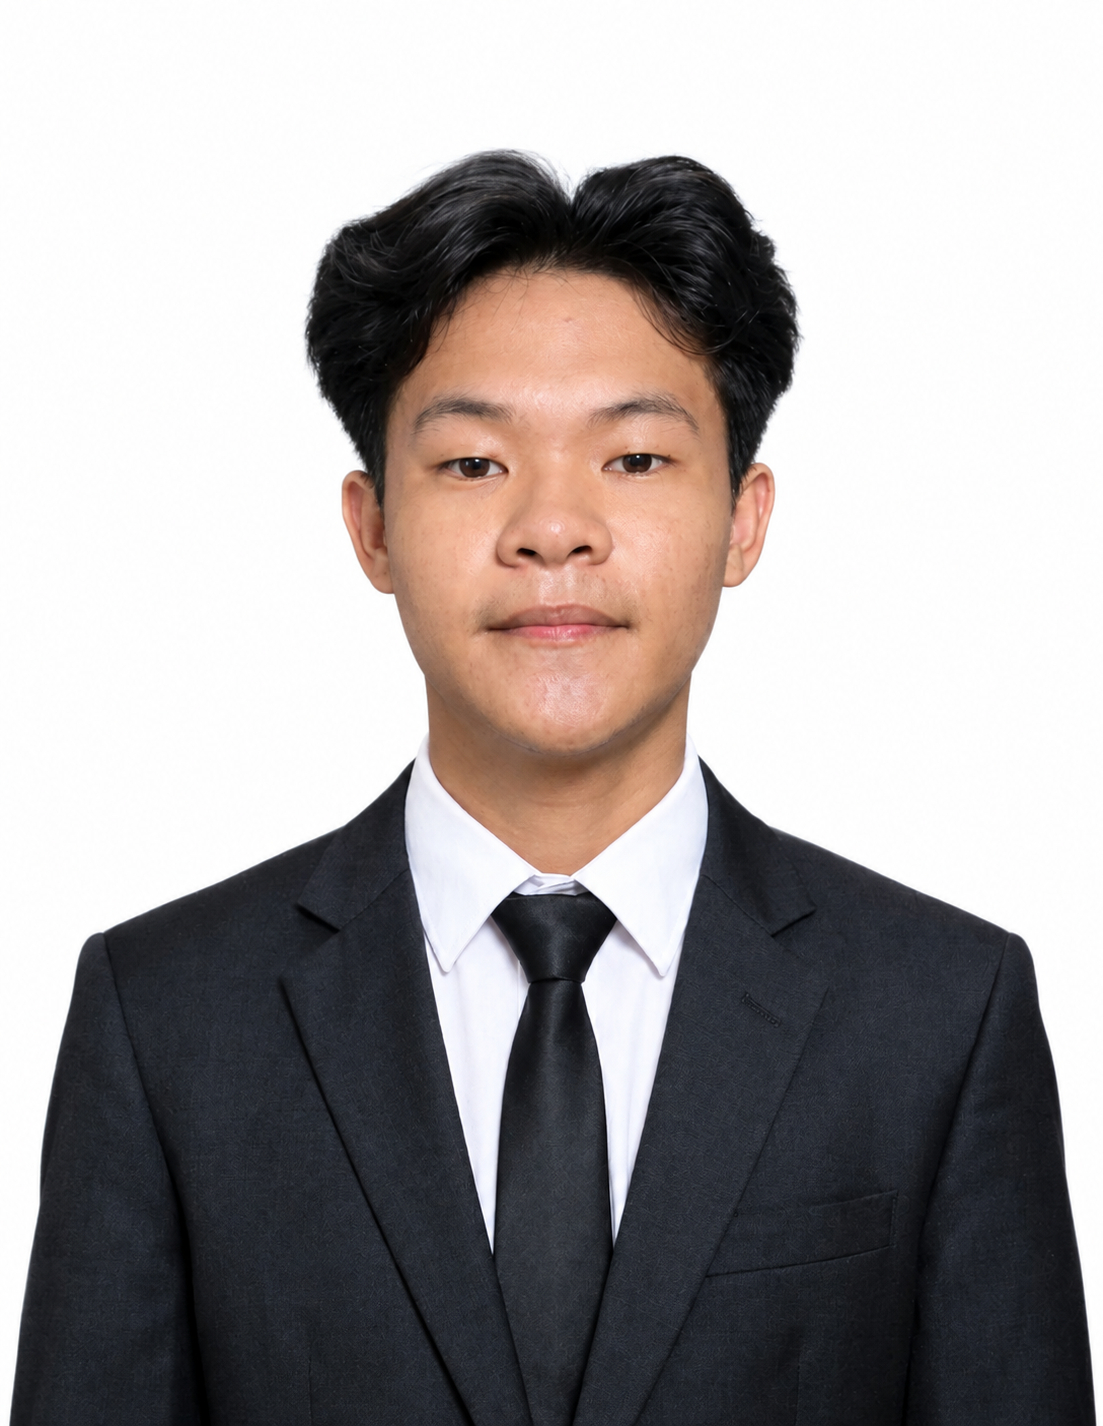
\includegraphics[width=1.5in,height=\textheight,keepaspectratio]{images/author/Jesen.png}

}

\caption{Jesen}

\end{figure}%

\textbf{\href{https://www.linkedin.com/in/jesenn}{Jesen}} adalah
mahasiswa S1 Program Studi Sains Data di Institut Teknologi Sains
Bandung (ITSB). Saat ini ia sedang aktif mempelajari Python, statistika,
R, analisis data, dan \emph{machine learning} sebagai fondasi untuk
memahami bagaimana data diolah menjadi informasi yang bermanfaat.

Ia tertarik pada kecerdasan buatan (\emph{Artificial Intelligence}) dan
penyelesaian masalah berbasis data, terutama bagaimana data dapat
dimanfaatkan untuk mendukung pengambilan keputusan. Dalam proses
belajarnya, ia terbiasa mempraktikkan langsung konsep yang dipelajari di
kelas melalui latihan dan tugas praktikum, termasuk yang dikumpulkan
dalam buku ini.

Buku \textbf{``Praktikum Pengantar Statistika''} ini menjadi salah satu
langkah awal dalam mendokumentasikan perjalanan belajarnya. Sebagai
mahasiswa yang masih terus belajar, ia terbuka terhadap masukan dan
koreksi dari pembaca. Repositori buku ini dapat dilihat di
\href{https://github.com/sennie17}{GitHub}.

\section*{Ucapan Terima Kasih}\label{ucapan-terima-kasih}
\addcontentsline{toc}{section}{Ucapan Terima Kasih}

\markright{Ucapan Terima Kasih}

Penyusunan eBook ini tidak terlepas dari bantuan dan dukungan berbagai
pihak. Dengan penuh rasa hormat, saya ingin mengucapkan terima kasih
kepada:

\begin{itemize}
\tightlist
\item
  \textbf{Mr.~Bakti Siregar, M.Sc.}, dosen pengampu mata kuliah
  Pengantar Statistika di \href{https://itsb.ac.id/}{Institut Teknologi
  Sains Bandung}, atas ilmu, bimbingan, dan kesabaran selama perkuliahan
  dan praktikum. Tanpa arahan beliau, buku ini tidak akan dapat
  tersusun.
\item
  \textbf{Para pembaca dan pengguna buku ini}, yang telah meluangkan
  waktu untuk membaca dan mempelajarinya. Kehadiran dan masukan Anda
  menjadi semangat bagi saya untuk terus belajar dan memperbaiki tulisan
  ini.
\end{itemize}

Saya berharap eBook ini dapat bermanfaat bagi siapa pun yang sedang
mempelajari statistika, khususnya sesama mahasiswa yang baru mulai
mengenal analisis data. Semoga ilmu yang tertuang di dalamnya dapat
memberi manfaat bagi kita semua.

\section*{Masukan \& Saran}\label{masukan-saran}
\addcontentsline{toc}{section}{Masukan \& Saran}

\markright{Masukan \& Saran}

Buku ini disusun oleh seorang mahasiswa yang masih terus belajar,
sehingga kritik, koreksi, dan saran dari pembaca sangat berarti untuk
perbaikan ke depan. Jika Anda menemukan kekeliruan atau memiliki usulan,
silakan sampaikan melalui kontak berikut:

\textbf{Email:}
\href{mailto:jesentriago08@gmail.com}{\nolinkurl{jesentriago08@gmail.com}}\\
\textbf{LinkedIn:} \href{https://www.linkedin.com/in/jesenn}{Jesen}\\
\textbf{GitHub:}
\href{https://github.com/sennie17/STATISITKA-EBOOK/issues}{Laporkan
masalah atau usulan}

\bookmarksetup{startatroot}

\chapter{Bab 9: Sampling Distribution dan
Estimasi}\label{bab-9-sampling-distribution-dan-estimasi}

\section{Tiga Distribusi yang Harus
Dibedakan}\label{tiga-distribusi-yang-harus-dibedakan}

{\def\LTcaptype{none} % do not increment counter
\begin{longtable}[]{@{}
  >{\raggedright\arraybackslash}p{(\linewidth - 6\tabcolsep) * \real{0.2500}}
  >{\raggedright\arraybackslash}p{(\linewidth - 6\tabcolsep) * \real{0.2500}}
  >{\raggedright\arraybackslash}p{(\linewidth - 6\tabcolsep) * \real{0.2500}}
  >{\raggedright\arraybackslash}p{(\linewidth - 6\tabcolsep) * \real{0.2500}}@{}}
\toprule\noalign{}
\begin{minipage}[b]{\linewidth}\raggedright
Distribusi
\end{minipage} & \begin{minipage}[b]{\linewidth}\raggedright
Isinya
\end{minipage} & \begin{minipage}[b]{\linewidth}\raggedright
Jumlah nilai
\end{minipage} & \begin{minipage}[b]{\linewidth}\raggedright
Contoh
\end{minipage} \\
\midrule\noalign{}
\endhead
\bottomrule\noalign{}
\endlastfoot
Distribusi populasi & Nilai setiap unit populasi & \(N\) & Pengeluaran
20.000 mahasiswa \\
Distribusi sampel & Nilai unit dalam satu sampel & \(n\) & Pengeluaran
40 mahasiswa yang disurvei \\
\textbf{Distribusi sampling} & Nilai \textbf{statistik} (misalnya
\(\bar{x}\)) dari banyak sampel (dibayangkan) & Sebanyak sampel yang
diambil & \(\bar{x}\) dari 10.000 sampel berukuran 40 \\
\end{longtable}
}

Distribusi sampling adalah konsep \textbf{teoretis}: dalam praktik kita
hanya memiliki satu sampel. Namun dengan simulasi kita dapat
``melihatnya''.

\subsection{Populasi Simulasi}\label{populasi-simulasi}

Kita memakai populasi 20.000 mahasiswa dengan variabel waktu layar
harian (jam) yang \textbf{menjulur kanan} -- bentuk yang sengaja dipilih
jauh dari lonceng.

\begin{Shaded}
\begin{Highlighting}[]
\FunctionTok{set.seed}\NormalTok{(}\DecValTok{909}\NormalTok{)}
\NormalTok{N }\OtherTok{\textless{}{-}} \DecValTok{20000}
\NormalTok{populasi }\OtherTok{\textless{}{-}} \FunctionTok{round}\NormalTok{(}\FunctionTok{rgamma}\NormalTok{(N, }\AttributeTok{shape =} \DecValTok{2}\NormalTok{, }\AttributeTok{rate =} \FloatTok{0.4}\NormalTok{), }\DecValTok{2}\NormalTok{)   }\CommentTok{\# jam per hari}
\NormalTok{mu    }\OtherTok{\textless{}{-}} \FunctionTok{mean}\NormalTok{(populasi)}
\NormalTok{sigma }\OtherTok{\textless{}{-}} \FunctionTok{sqrt}\NormalTok{(}\FunctionTok{mean}\NormalTok{((populasi }\SpecialCharTok{{-}}\NormalTok{ mu)}\SpecialCharTok{\^{}}\DecValTok{2}\NormalTok{))                   }\CommentTok{\# SD populasi (pembagi N)}

\FunctionTok{c}\NormalTok{(}\AttributeTok{N =}\NormalTok{ N, }\AttributeTok{mu =} \FunctionTok{round}\NormalTok{(mu, }\DecValTok{3}\NormalTok{), }\AttributeTok{sigma =} \FunctionTok{round}\NormalTok{(sigma, }\DecValTok{3}\NormalTok{))}
\end{Highlighting}
\end{Shaded}

\begin{verbatim}
        N        mu     sigma 
20000.000     5.010     3.551 
\end{verbatim}

\begin{Shaded}
\begin{Highlighting}[]
\FunctionTok{set.seed}\NormalTok{(}\DecValTok{1}\NormalTok{)}
\NormalTok{satu\_sampel }\OtherTok{\textless{}{-}} \FunctionTok{sample}\NormalTok{(populasi, }\DecValTok{40}\NormalTok{)}
\NormalTok{banyak\_rata }\OtherTok{\textless{}{-}} \FunctionTok{replicate}\NormalTok{(}\DecValTok{10000}\NormalTok{, }\FunctionTok{mean}\NormalTok{(}\FunctionTok{sample}\NormalTok{(populasi, }\DecValTok{40}\NormalTok{)))}

\FunctionTok{par}\NormalTok{(}\AttributeTok{mfrow =} \FunctionTok{c}\NormalTok{(}\DecValTok{1}\NormalTok{, }\DecValTok{3}\NormalTok{))}
\FunctionTok{hist}\NormalTok{(populasi, }\AttributeTok{breaks =} \DecValTok{40}\NormalTok{, }\AttributeTok{col =} \StringTok{"\#9ecae1"}\NormalTok{, }\AttributeTok{border =} \StringTok{"white"}\NormalTok{, }\AttributeTok{main =} \StringTok{"Populasi (N = 20.000)"}\NormalTok{,}
     \AttributeTok{xlab =} \StringTok{"Jam per hari"}\NormalTok{, }\AttributeTok{xlim =} \FunctionTok{c}\NormalTok{(}\DecValTok{0}\NormalTok{, }\DecValTok{20}\NormalTok{))}
\FunctionTok{hist}\NormalTok{(satu\_sampel, }\AttributeTok{breaks =} \DecValTok{12}\NormalTok{, }\AttributeTok{col =} \StringTok{"\#fdae6b"}\NormalTok{, }\AttributeTok{border =} \StringTok{"white"}\NormalTok{, }\AttributeTok{main =} \StringTok{"Satu sampel (n = 40)"}\NormalTok{,}
     \AttributeTok{xlab =} \StringTok{"Jam per hari"}\NormalTok{, }\AttributeTok{xlim =} \FunctionTok{c}\NormalTok{(}\DecValTok{0}\NormalTok{, }\DecValTok{20}\NormalTok{))}
\FunctionTok{hist}\NormalTok{(banyak\_rata, }\AttributeTok{breaks =} \DecValTok{40}\NormalTok{, }\AttributeTok{col =} \StringTok{"\#a1d99b"}\NormalTok{, }\AttributeTok{border =} \StringTok{"white"}\NormalTok{,}
     \AttributeTok{main =} \StringTok{"Sampling distribution x{-}bar"}\NormalTok{, }\AttributeTok{xlab =} \StringTok{"Rata{-}rata sampel (n = 40)"}\NormalTok{)}
\end{Highlighting}
\end{Shaded}

\begin{center}
\includegraphics[width=1\linewidth,height=\textheight,keepaspectratio]{chapters/bab-9_files/figure-pdf/unnamed-chunk-2-1.pdf}
\end{center}

\begin{Shaded}
\begin{Highlighting}[]
\FunctionTok{par}\NormalTok{(}\AttributeTok{mfrow =} \FunctionTok{c}\NormalTok{(}\DecValTok{1}\NormalTok{, }\DecValTok{1}\NormalTok{))}
\end{Highlighting}
\end{Shaded}

Populasi dan satu sampel sama-sama menjulur kanan, tetapi
\textbf{distribusi rata-rata sampel} jauh lebih sempit dan hampir
berbentuk lonceng. Inilah inti pertemuan ini.

\section{Distribusi Sampling Rata-rata
Sampel}\label{distribusi-sampling-rata-rata-sampel}

Untuk sampel acak berukuran \(n\) dari populasi dengan mean \(\mu\) dan
simpangan baku \(\sigma\):

{\def\LTcaptype{none} % do not increment counter
\begin{longtable}[]{@{}
  >{\raggedright\arraybackslash}p{(\linewidth - 4\tabcolsep) * \real{0.3333}}
  >{\raggedright\arraybackslash}p{(\linewidth - 4\tabcolsep) * \real{0.3333}}
  >{\raggedright\arraybackslash}p{(\linewidth - 4\tabcolsep) * \real{0.3333}}@{}}
\toprule\noalign{}
\begin{minipage}[b]{\linewidth}\raggedright
Sifat
\end{minipage} & \begin{minipage}[b]{\linewidth}\raggedright
Rumus
\end{minipage} & \begin{minipage}[b]{\linewidth}\raggedright
Arti
\end{minipage} \\
\midrule\noalign{}
\endhead
\bottomrule\noalign{}
\endlastfoot
\textbf{Mean} & \(\mu_{\bar{x}} = \mu\) & \(\bar{x}\) adalah penaksir
\textbf{tak bias}: rata-ratanya tepat di parameter \\
\textbf{Standard error} &
\(\sigma_{\bar{x}} = \dfrac{\sigma}{\sqrt{n}}\) & Sebaran \(\bar{x}\)
mengecil seiring bertambahnya \(n\) \\
\textbf{Bentuk} & Normal jika populasi normal; mendekati normal untuk
\(n\) cukup besar (CLT) & Memungkinkan perhitungan peluang \\
\end{longtable}
}

\begin{Shaded}
\begin{Highlighting}[]
\FunctionTok{kable}\NormalTok{(}\FunctionTok{data.frame}\NormalTok{(}
  \AttributeTok{Besaran =} \FunctionTok{c}\NormalTok{(}\StringTok{"Mean distribusi sampling"}\NormalTok{, }\StringTok{"SD distribusi sampling (SE)"}\NormalTok{),}
  \AttributeTok{Teori   =} \FunctionTok{round}\NormalTok{(}\FunctionTok{c}\NormalTok{(mu, sigma }\SpecialCharTok{/} \FunctionTok{sqrt}\NormalTok{(}\DecValTok{40}\NormalTok{)), }\DecValTok{4}\NormalTok{),}
  \AttributeTok{Simulasi\_10000\_sampel =} \FunctionTok{round}\NormalTok{(}\FunctionTok{c}\NormalTok{(}\FunctionTok{mean}\NormalTok{(banyak\_rata), }\FunctionTok{sd}\NormalTok{(banyak\_rata)), }\DecValTok{4}\NormalTok{)}
\NormalTok{), }\AttributeTok{caption =} \StringTok{"Teori vs simulasi untuk n = 40"}\NormalTok{)}
\end{Highlighting}
\end{Shaded}

\begin{longtable}[]{@{}lrr@{}}
\caption{Teori vs simulasi untuk n = 40}\tabularnewline
\toprule\noalign{}
Besaran & Teori & Simulasi\_10000\_sampel \\
\midrule\noalign{}
\endfirsthead
\toprule\noalign{}
Besaran & Teori & Simulasi\_10000\_sampel \\
\midrule\noalign{}
\endhead
\bottomrule\noalign{}
\endlastfoot
Mean distribusi sampling & 5.0097 & 5.0024 \\
SD distribusi sampling (SE) & 0.5615 & 0.5556 \\
\end{longtable}

Hasil simulasi hampir persis sama dengan teori.

\textbf{Koreksi populasi terhingga.} Rumus \(\sigma/\sqrt{n}\)
mengasumsikan populasi sangat besar dibanding sampel. Jika sampel
mencapai lebih dari sekitar 5\% populasi (tanpa pengembalian), SE
dikalikan faktor \(\sqrt{\dfrac{N-n}{N-1}}\). Pada contoh ini
\(n/N = 0{,}2\%\), sehingga koreksi dapat diabaikan.

\subsection{Pengaruh Ukuran Sampel}\label{pengaruh-ukuran-sampel}

\begin{Shaded}
\begin{Highlighting}[]
\FunctionTok{set.seed}\NormalTok{(}\DecValTok{2}\NormalTok{)}
\NormalTok{n\_list }\OtherTok{\textless{}{-}} \FunctionTok{c}\NormalTok{(}\DecValTok{5}\NormalTok{, }\DecValTok{20}\NormalTok{, }\DecValTok{80}\NormalTok{)}
\FunctionTok{par}\NormalTok{(}\AttributeTok{mfrow =} \FunctionTok{c}\NormalTok{(}\DecValTok{1}\NormalTok{, }\DecValTok{3}\NormalTok{))}
\ControlFlowTok{for}\NormalTok{ (nn }\ControlFlowTok{in}\NormalTok{ n\_list) \{}
\NormalTok{  rata }\OtherTok{\textless{}{-}} \FunctionTok{replicate}\NormalTok{(}\DecValTok{5000}\NormalTok{, }\FunctionTok{mean}\NormalTok{(}\FunctionTok{sample}\NormalTok{(populasi, nn)))}
  \FunctionTok{hist}\NormalTok{(rata, }\AttributeTok{breaks =} \DecValTok{40}\NormalTok{, }\AttributeTok{col =} \StringTok{"\#a1d99b"}\NormalTok{, }\AttributeTok{border =} \StringTok{"white"}\NormalTok{, }\AttributeTok{xlim =} \FunctionTok{c}\NormalTok{(}\DecValTok{1}\NormalTok{, }\DecValTok{10}\NormalTok{), }\AttributeTok{freq =} \ConstantTok{FALSE}\NormalTok{,}
       \AttributeTok{main =} \FunctionTok{paste0}\NormalTok{(}\StringTok{"n = "}\NormalTok{, nn, }\StringTok{"  (SE = "}\NormalTok{, }\FunctionTok{round}\NormalTok{(sigma }\SpecialCharTok{/} \FunctionTok{sqrt}\NormalTok{(nn), }\DecValTok{2}\NormalTok{), }\StringTok{")"}\NormalTok{),}
       \AttributeTok{xlab =} \StringTok{"Rata{-}rata sampel"}\NormalTok{)}
  \FunctionTok{curve}\NormalTok{(}\FunctionTok{dnorm}\NormalTok{(x, mu, sigma }\SpecialCharTok{/} \FunctionTok{sqrt}\NormalTok{(nn)), }\AttributeTok{add =} \ConstantTok{TRUE}\NormalTok{, }\AttributeTok{col =} \StringTok{"firebrick"}\NormalTok{, }\AttributeTok{lwd =} \DecValTok{2}\NormalTok{)}
  \FunctionTok{abline}\NormalTok{(}\AttributeTok{v =}\NormalTok{ mu, }\AttributeTok{lty =} \DecValTok{2}\NormalTok{)}
\NormalTok{\}}
\end{Highlighting}
\end{Shaded}

\begin{center}
\includegraphics[width=1\linewidth,height=\textheight,keepaspectratio]{chapters/bab-9_files/figure-pdf/unnamed-chunk-4-1.pdf}
\end{center}

\begin{Shaded}
\begin{Highlighting}[]
\FunctionTok{par}\NormalTok{(}\AttributeTok{mfrow =} \FunctionTok{c}\NormalTok{(}\DecValTok{1}\NormalTok{, }\DecValTok{1}\NormalTok{))}
\end{Highlighting}
\end{Shaded}

Kurva merah adalah distribusi normal dengan mean \(\mu\) dan SD
\(\sigma/\sqrt{n}\). Semakin besar \(n\): (1) distribusi semakin
\textbf{sempit}, dan (2) bentuknya semakin \textbf{mendekati normal}
meskipun populasinya menjulur kanan.

\section{Central Limit Theorem (CLT)}\label{central-limit-theorem-clt}

\textbf{Central Limit Theorem.} Jika sampel acak berukuran \(n\) diambil
dari populasi \textbf{sembarang bentuk} dengan mean \(\mu\) dan
simpangan baku \(\sigma\) (terhingga), maka untuk \(n\) yang cukup
besar, distribusi sampling \(\bar{x}\) mendekati normal:

\[\bar{x} \approx N\left(\mu,\ \frac{\sigma}{\sqrt{n}}\right)\]

CLT adalah alasan mengapa distribusi normal muncul di mana-mana dalam
statistika inferensial -- bukan karena data selalu normal, tetapi karena
\textbf{rata-rata} dari data cenderung normal.

\subsection{Demonstrasi pada Tiga Bentuk
Populasi}\label{demonstrasi-pada-tiga-bentuk-populasi}

\begin{Shaded}
\begin{Highlighting}[]
\FunctionTok{set.seed}\NormalTok{(}\DecValTok{3}\NormalTok{)}
\NormalTok{pop\_bentuk }\OtherTok{\textless{}{-}} \FunctionTok{list}\NormalTok{(}
  \StringTok{"Seragam"}        \OtherTok{=} \FunctionTok{runif}\NormalTok{(}\DecValTok{20000}\NormalTok{, }\DecValTok{0}\NormalTok{, }\DecValTok{10}\NormalTok{),}
  \StringTok{"Menjulur kanan"} \OtherTok{=} \FunctionTok{rexp}\NormalTok{(}\DecValTok{20000}\NormalTok{, }\AttributeTok{rate =} \FloatTok{0.5}\NormalTok{),}
  \StringTok{"Bimodal"}        \OtherTok{=} \FunctionTok{c}\NormalTok{(}\FunctionTok{rnorm}\NormalTok{(}\DecValTok{10000}\NormalTok{, }\DecValTok{2}\NormalTok{, }\FloatTok{0.8}\NormalTok{), }\FunctionTok{rnorm}\NormalTok{(}\DecValTok{10000}\NormalTok{, }\DecValTok{8}\NormalTok{, }\FloatTok{0.8}\NormalTok{))}
\NormalTok{)}
\NormalTok{ukuran }\OtherTok{\textless{}{-}} \FunctionTok{c}\NormalTok{(}\DecValTok{2}\NormalTok{, }\DecValTok{5}\NormalTok{, }\DecValTok{30}\NormalTok{)}

\FunctionTok{par}\NormalTok{(}\AttributeTok{mfrow =} \FunctionTok{c}\NormalTok{(}\DecValTok{4}\NormalTok{, }\DecValTok{3}\NormalTok{), }\AttributeTok{mar =} \FunctionTok{c}\NormalTok{(}\DecValTok{3}\NormalTok{, }\DecValTok{3}\NormalTok{, }\FloatTok{2.5}\NormalTok{, }\DecValTok{1}\NormalTok{))}
\ControlFlowTok{for}\NormalTok{ (nama }\ControlFlowTok{in} \FunctionTok{names}\NormalTok{(pop\_bentuk)) \{}
  \FunctionTok{hist}\NormalTok{(pop\_bentuk[[nama]], }\AttributeTok{breaks =} \DecValTok{40}\NormalTok{, }\AttributeTok{col =} \StringTok{"\#9ecae1"}\NormalTok{, }\AttributeTok{border =} \StringTok{"white"}\NormalTok{,}
       \AttributeTok{main =} \FunctionTok{paste}\NormalTok{(}\StringTok{"Populasi:"}\NormalTok{, nama), }\AttributeTok{xlab =} \StringTok{""}\NormalTok{, }\AttributeTok{ylab =} \StringTok{""}\NormalTok{)}
\NormalTok{\}}
\ControlFlowTok{for}\NormalTok{ (nn }\ControlFlowTok{in}\NormalTok{ ukuran) \{}
  \ControlFlowTok{for}\NormalTok{ (nama }\ControlFlowTok{in} \FunctionTok{names}\NormalTok{(pop\_bentuk)) \{}
\NormalTok{    rata }\OtherTok{\textless{}{-}} \FunctionTok{replicate}\NormalTok{(}\DecValTok{3000}\NormalTok{, }\FunctionTok{mean}\NormalTok{(}\FunctionTok{sample}\NormalTok{(pop\_bentuk[[nama]], nn)))}
    \FunctionTok{hist}\NormalTok{(rata, }\AttributeTok{breaks =} \DecValTok{35}\NormalTok{, }\AttributeTok{col =} \StringTok{"\#a1d99b"}\NormalTok{, }\AttributeTok{border =} \StringTok{"white"}\NormalTok{,}
         \AttributeTok{main =} \FunctionTok{paste0}\NormalTok{(nama, }\StringTok{", n = "}\NormalTok{, nn), }\AttributeTok{xlab =} \StringTok{""}\NormalTok{, }\AttributeTok{ylab =} \StringTok{""}\NormalTok{)}
\NormalTok{  \}}
\NormalTok{\}}
\end{Highlighting}
\end{Shaded}

\begin{center}
\includegraphics[width=1\linewidth,height=\textheight,keepaspectratio]{chapters/bab-9_files/figure-pdf/unnamed-chunk-5-1.pdf}
\end{center}

\begin{Shaded}
\begin{Highlighting}[]
\FunctionTok{par}\NormalTok{(}\AttributeTok{mfrow =} \FunctionTok{c}\NormalTok{(}\DecValTok{1}\NormalTok{, }\DecValTok{1}\NormalTok{), }\AttributeTok{mar =} \FunctionTok{c}\NormalTok{(}\DecValTok{5}\NormalTok{, }\DecValTok{4}\NormalTok{, }\DecValTok{4}\NormalTok{, }\DecValTok{2}\NormalTok{) }\SpecialCharTok{+} \FloatTok{0.1}\NormalTok{)}
\end{Highlighting}
\end{Shaded}

Baris pertama adalah populasi; baris berikutnya adalah distribusi
sampling \(\bar{x}\) untuk \(n = 2\), 5, dan 30. Populasi
\textbf{seragam} sudah tampak lonceng pada \(n = 5\); populasi
\textbf{bimodal} masih bergelombang pada \(n = 2\) tetapi lonceng pada
\(n = 30\); populasi \textbf{menjulur kanan} membutuhkan \(n\) terbesar
untuk menghilangkan kemencengannya.

\subsection{Seberapa Besar ``Cukup
Besar''?}\label{seberapa-besar-cukup-besar}

{\def\LTcaptype{none} % do not increment counter
\begin{longtable}[]{@{}ll@{}}
\toprule\noalign{}
Bentuk populasi & Ukuran sampel yang biasanya cukup \\
\midrule\noalign{}
\endhead
\bottomrule\noalign{}
\endlastfoot
Normal & Berapa pun (distribusi \(\bar{x}\) tepat normal) \\
Simetris, tidak normal & Sekitar 10--15 \\
Menceng sedang & Sekitar 30 (aturan praktis yang populer) \\
Sangat menceng atau banyak outlier & Bisa jauh lebih dari 30 \\
\end{longtable}
}

\begin{Shaded}
\begin{Highlighting}[]
\NormalTok{skew }\OtherTok{\textless{}{-}} \ControlFlowTok{function}\NormalTok{(x) \{ d }\OtherTok{\textless{}{-}}\NormalTok{ x }\SpecialCharTok{{-}} \FunctionTok{mean}\NormalTok{(x); }\FunctionTok{mean}\NormalTok{(d}\SpecialCharTok{\^{}}\DecValTok{3}\NormalTok{) }\SpecialCharTok{/} \FunctionTok{mean}\NormalTok{(d}\SpecialCharTok{\^{}}\DecValTok{2}\NormalTok{)}\SpecialCharTok{\^{}}\FloatTok{1.5}\NormalTok{ \}}
\FunctionTok{set.seed}\NormalTok{(}\DecValTok{4}\NormalTok{)}
\FunctionTok{data.frame}\NormalTok{(}\AttributeTok{n =} \FunctionTok{c}\NormalTok{(}\DecValTok{2}\NormalTok{, }\DecValTok{5}\NormalTok{, }\DecValTok{10}\NormalTok{, }\DecValTok{30}\NormalTok{, }\DecValTok{100}\NormalTok{),}
           \AttributeTok{Kemencengan\_xbar =} \FunctionTok{sapply}\NormalTok{(}\FunctionTok{c}\NormalTok{(}\DecValTok{2}\NormalTok{, }\DecValTok{5}\NormalTok{, }\DecValTok{10}\NormalTok{, }\DecValTok{30}\NormalTok{, }\DecValTok{100}\NormalTok{), }\ControlFlowTok{function}\NormalTok{(nn)}
             \FunctionTok{round}\NormalTok{(}\FunctionTok{skew}\NormalTok{(}\FunctionTok{replicate}\NormalTok{(}\DecValTok{5000}\NormalTok{, }\FunctionTok{mean}\NormalTok{(}\FunctionTok{sample}\NormalTok{(populasi, nn)))), }\DecValTok{3}\NormalTok{)))}
\end{Highlighting}
\end{Shaded}

\begin{verbatim}
    n Kemencengan_xbar
1   2            1.007
2   5            0.581
3  10            0.470
4  30            0.220
5 100            0.170
\end{verbatim}

Kemencengan distribusi \(\bar{x}\) menyusut kira-kira sebanding dengan
\(1/\sqrt{n}\).

\subsection{Menghitung Peluang dengan
CLT}\label{menghitung-peluang-dengan-clt}

Contoh: Jika diambil sampel acak 40 mahasiswa, berapa peluang rata-rata
waktu layarnya melebihi 5,5 jam?

\[z = \frac{\bar{x} - \mu}{\sigma / \sqrt{n}} \qquad\qquad P(\bar{x} > 5{,}5) = P(Z > z)\]

\begin{Shaded}
\begin{Highlighting}[]
\NormalTok{se40  }\OtherTok{\textless{}{-}}\NormalTok{ sigma }\SpecialCharTok{/} \FunctionTok{sqrt}\NormalTok{(}\DecValTok{40}\NormalTok{)}
\NormalTok{z\_55  }\OtherTok{\textless{}{-}}\NormalTok{ (}\FloatTok{5.5} \SpecialCharTok{{-}}\NormalTok{ mu) }\SpecialCharTok{/}\NormalTok{ se40}

\FunctionTok{c}\NormalTok{(}\AttributeTok{SE =} \FunctionTok{round}\NormalTok{(se40, }\DecValTok{4}\NormalTok{), }\AttributeTok{z =} \FunctionTok{round}\NormalTok{(z\_55, }\DecValTok{3}\NormalTok{),}
  \AttributeTok{Peluang\_CLT      =} \FunctionTok{round}\NormalTok{(}\DecValTok{1} \SpecialCharTok{{-}} \FunctionTok{pnorm}\NormalTok{(z\_55), }\DecValTok{4}\NormalTok{),}
  \AttributeTok{Peluang\_simulasi =} \FunctionTok{round}\NormalTok{(}\FunctionTok{mean}\NormalTok{(banyak\_rata }\SpecialCharTok{\textgreater{}} \FloatTok{5.5}\NormalTok{), }\DecValTok{4}\NormalTok{))}
\end{Highlighting}
\end{Shaded}

\begin{verbatim}
              SE                z      Peluang_CLT Peluang_simulasi 
          0.5615           0.8730           0.1913           0.1803 
\end{verbatim}

Perbandingan: peluang \textbf{seorang} mahasiswa (bukan rata-rata 40
orang) memiliki waktu layar di atas 5,5 jam jauh lebih besar:

\begin{Shaded}
\begin{Highlighting}[]
\FunctionTok{mean}\NormalTok{(populasi }\SpecialCharTok{\textgreater{}} \FloatTok{5.5}\NormalTok{)}
\end{Highlighting}
\end{Shaded}

\begin{verbatim}
[1] 0.35175
\end{verbatim}

Individu sangat bervariasi, tetapi rata-rata dari banyak individu jauh
lebih stabil.

\section{Distribusi Sampling Proporsi
Sampel}\label{distribusi-sampling-proporsi-sampel}

Untuk variabel kategorik biner (Ya/Tidak), statistik yang dipakai adalah
proporsi sampel \(\hat{p} = x/n\).

{\def\LTcaptype{none} % do not increment counter
\begin{longtable}[]{@{}ll@{}}
\toprule\noalign{}
Sifat & Rumus \\
\midrule\noalign{}
\endhead
\bottomrule\noalign{}
\endlastfoot
Mean & \(\mu_{\hat{p}} = p\) \\
Standard error & \(\sigma_{\hat{p}} = \sqrt{\dfrac{p(1-p)}{n}}\) \\
Bentuk & Mendekati normal jika \(np \geq 10\) \textbf{dan}
\(n(1-p) \geq 10\) \\
\end{longtable}
}

\begin{Shaded}
\begin{Highlighting}[]
\NormalTok{p\_benar }\OtherTok{\textless{}{-}} \FloatTok{0.08}    \CommentTok{\# misalnya 8\% mahasiswa pernah terlambat membayar UKT}
\FunctionTok{set.seed}\NormalTok{(}\DecValTok{5}\NormalTok{)}
\FunctionTok{par}\NormalTok{(}\AttributeTok{mfrow =} \FunctionTok{c}\NormalTok{(}\DecValTok{1}\NormalTok{, }\DecValTok{3}\NormalTok{))}
\ControlFlowTok{for}\NormalTok{ (nn }\ControlFlowTok{in} \FunctionTok{c}\NormalTok{(}\DecValTok{20}\NormalTok{, }\DecValTok{60}\NormalTok{, }\DecValTok{300}\NormalTok{)) \{}
\NormalTok{  p\_hat }\OtherTok{\textless{}{-}} \FunctionTok{rbinom}\NormalTok{(}\DecValTok{5000}\NormalTok{, }\AttributeTok{size =}\NormalTok{ nn, }\AttributeTok{prob =}\NormalTok{ p\_benar) }\SpecialCharTok{/}\NormalTok{ nn}
  \FunctionTok{hist}\NormalTok{(p\_hat, }\AttributeTok{breaks =} \FunctionTok{seq}\NormalTok{(}\SpecialCharTok{{-}}\FloatTok{0.005}\NormalTok{, }\FloatTok{0.4}\NormalTok{, }\AttributeTok{by =} \FloatTok{0.01}\NormalTok{), }\AttributeTok{col =} \StringTok{"\#fdae6b"}\NormalTok{, }\AttributeTok{border =} \StringTok{"white"}\NormalTok{,}
       \AttributeTok{freq =} \ConstantTok{FALSE}\NormalTok{, }\AttributeTok{xlim =} \FunctionTok{c}\NormalTok{(}\DecValTok{0}\NormalTok{, }\FloatTok{0.3}\NormalTok{),}
       \AttributeTok{main =} \FunctionTok{paste0}\NormalTok{(}\StringTok{"n = "}\NormalTok{, nn, }\StringTok{": np = "}\NormalTok{, nn }\SpecialCharTok{*}\NormalTok{ p\_benar), }\AttributeTok{xlab =} \StringTok{"Proporsi sampel"}\NormalTok{)}
  \FunctionTok{curve}\NormalTok{(}\FunctionTok{dnorm}\NormalTok{(x, p\_benar, }\FunctionTok{sqrt}\NormalTok{(p\_benar }\SpecialCharTok{*}\NormalTok{ (}\DecValTok{1} \SpecialCharTok{{-}}\NormalTok{ p\_benar) }\SpecialCharTok{/}\NormalTok{ nn)), }\AttributeTok{add =} \ConstantTok{TRUE}\NormalTok{,}
        \AttributeTok{col =} \StringTok{"firebrick"}\NormalTok{, }\AttributeTok{lwd =} \DecValTok{2}\NormalTok{)}
\NormalTok{\}}
\end{Highlighting}
\end{Shaded}

\begin{center}
\includegraphics[width=1\linewidth,height=\textheight,keepaspectratio]{chapters/bab-9_files/figure-pdf/unnamed-chunk-9-1.pdf}
\end{center}

\begin{Shaded}
\begin{Highlighting}[]
\FunctionTok{par}\NormalTok{(}\AttributeTok{mfrow =} \FunctionTok{c}\NormalTok{(}\DecValTok{1}\NormalTok{, }\DecValTok{1}\NormalTok{))}
\end{Highlighting}
\end{Shaded}

Dengan \(n = 20\) (\(np = 1{,}6\)), distribusi \(\hat{p}\) sangat
menceng dan ``berbatang'' -- pendekatan normal \textbf{buruk}. Dengan
\(n = 300\) (\(np = 24\)), pendekatan normal \textbf{sangat baik}.

\section{Standard Error}\label{standard-error}

\subsection{Standard Error vs Simpangan
Baku}\label{standard-error-vs-simpangan-baku}

{\def\LTcaptype{none} % do not increment counter
\begin{longtable}[]{@{}
  >{\raggedright\arraybackslash}p{(\linewidth - 4\tabcolsep) * \real{0.3333}}
  >{\raggedright\arraybackslash}p{(\linewidth - 4\tabcolsep) * \real{0.3333}}
  >{\raggedright\arraybackslash}p{(\linewidth - 4\tabcolsep) * \real{0.3333}}@{}}
\toprule\noalign{}
\begin{minipage}[b]{\linewidth}\raggedright
\end{minipage} & \begin{minipage}[b]{\linewidth}\raggedright
Simpangan baku (\(s\) atau \(\sigma\))
\end{minipage} & \begin{minipage}[b]{\linewidth}\raggedright
Standard error (\(SE\))
\end{minipage} \\
\midrule\noalign{}
\endhead
\bottomrule\noalign{}
\endlastfoot
\textbf{Mengukur sebaran} & Data individu & Statistik (misalnya
\(\bar{x}\)) dari sampel ke sampel \\
\textbf{Menjawab} & ``Seberapa beragam individu?'' & ``Seberapa tepat
taksiran kita?'' \\
\textbf{Jika \(n\) bertambah} & Tetap (mendekati \(\sigma\)) &
Mengecil \\
\textbf{Rumus (mean)} &
\(s = \sqrt{\dfrac{\sum (x_i - \bar{x})^2}{n-1}}\) &
\(SE = \dfrac{s}{\sqrt{n}}\) \\
\end{longtable}
}

Karena \(\sigma\) biasanya tidak diketahui, SE ditaksir dengan
\(s/\sqrt{n}\) (untuk mean) atau \(\sqrt{\hat{p}(1-\hat{p})/n}\) (untuk
proporsi).

\begin{Shaded}
\begin{Highlighting}[]
\FunctionTok{set.seed}\NormalTok{(}\DecValTok{6}\NormalTok{)}
\NormalTok{n\_besar }\OtherTok{\textless{}{-}} \FunctionTok{c}\NormalTok{(}\DecValTok{10}\NormalTok{, }\DecValTok{40}\NormalTok{, }\DecValTok{160}\NormalTok{, }\DecValTok{640}\NormalTok{)}
\FunctionTok{kable}\NormalTok{(}\FunctionTok{t}\NormalTok{(}\FunctionTok{sapply}\NormalTok{(n\_besar, }\ControlFlowTok{function}\NormalTok{(nn) \{}
\NormalTok{  hasil }\OtherTok{\textless{}{-}} \FunctionTok{replicate}\NormalTok{(}\DecValTok{2000}\NormalTok{, \{ s }\OtherTok{\textless{}{-}} \FunctionTok{sample}\NormalTok{(populasi, nn); }\FunctionTok{c}\NormalTok{(}\FunctionTok{sd}\NormalTok{(s), }\FunctionTok{sd}\NormalTok{(s) }\SpecialCharTok{/} \FunctionTok{sqrt}\NormalTok{(nn)) \})}
  \FunctionTok{c}\NormalTok{(}\AttributeTok{n =}\NormalTok{ nn, }\AttributeTok{Rata\_SD\_sampel =} \FunctionTok{round}\NormalTok{(}\FunctionTok{mean}\NormalTok{(hasil[}\DecValTok{1}\NormalTok{, ]), }\DecValTok{3}\NormalTok{),}
    \AttributeTok{Rata\_SE\_taksiran =} \FunctionTok{round}\NormalTok{(}\FunctionTok{mean}\NormalTok{(hasil[}\DecValTok{2}\NormalTok{, ]), }\DecValTok{3}\NormalTok{))}
\NormalTok{\})), }\AttributeTok{caption =} \FunctionTok{paste0}\NormalTok{(}\StringTok{"Rata{-}rata dari 2.000 sampel per n: SD stabil di sekitar sigma = "}\NormalTok{,}
                      \FunctionTok{round}\NormalTok{(sigma, }\DecValTok{2}\NormalTok{), }\StringTok{", SE mengecil"}\NormalTok{))}
\end{Highlighting}
\end{Shaded}

\begin{longtable}[]{@{}rrr@{}}
\caption{Rata-rata dari 2.000 sampel per n: SD stabil di sekitar sigma =
3.55, SE mengecil}\tabularnewline
\toprule\noalign{}
n & Rata\_SD\_sampel & Rata\_SE\_taksiran \\
\midrule\noalign{}
\endfirsthead
\toprule\noalign{}
n & Rata\_SD\_sampel & Rata\_SE\_taksiran \\
\midrule\noalign{}
\endhead
\bottomrule\noalign{}
\endlastfoot
10 & 3.348 & 1.059 \\
40 & 3.493 & 0.552 \\
160 & 3.537 & 0.280 \\
640 & 3.551 & 0.140 \\
\end{longtable}

\subsection{Hukum Akar Kuadrat}\label{hukum-akar-kuadrat}

Karena \(SE \propto 1/\sqrt{n}\), untuk \textbf{membagi dua SE}
dibutuhkan sampel \textbf{empat kali lipat}. Presisi semakin mahal:
menambah \(n\) dari 100 ke 400 memberi keuntungan yang sama dengan dari
400 ke 1.600.

\begin{Shaded}
\begin{Highlighting}[]
\NormalTok{n\_seq }\OtherTok{\textless{}{-}} \DecValTok{10}\SpecialCharTok{:}\DecValTok{1000}
\FunctionTok{plot}\NormalTok{(n\_seq, sigma }\SpecialCharTok{/} \FunctionTok{sqrt}\NormalTok{(n\_seq), }\AttributeTok{type =} \StringTok{"l"}\NormalTok{, }\AttributeTok{lwd =} \DecValTok{2}\NormalTok{, }\AttributeTok{col =} \StringTok{"\#4C72B0"}\NormalTok{,}
     \AttributeTok{xlab =} \StringTok{"Ukuran sampel (n)"}\NormalTok{, }\AttributeTok{ylab =} \StringTok{"Standard error"}\NormalTok{,}
     \AttributeTok{main =} \StringTok{"SE Menurun Cepat di Awal, Lalu Melandai"}\NormalTok{)}
\FunctionTok{points}\NormalTok{(}\FunctionTok{c}\NormalTok{(}\DecValTok{100}\NormalTok{, }\DecValTok{400}\NormalTok{), sigma }\SpecialCharTok{/} \FunctionTok{sqrt}\NormalTok{(}\FunctionTok{c}\NormalTok{(}\DecValTok{100}\NormalTok{, }\DecValTok{400}\NormalTok{)), }\AttributeTok{pch =} \DecValTok{16}\NormalTok{, }\AttributeTok{col =} \StringTok{"firebrick"}\NormalTok{, }\AttributeTok{cex =} \FloatTok{1.3}\NormalTok{)}
\FunctionTok{text}\NormalTok{(}\FunctionTok{c}\NormalTok{(}\DecValTok{100}\NormalTok{, }\DecValTok{400}\NormalTok{), sigma }\SpecialCharTok{/} \FunctionTok{sqrt}\NormalTok{(}\FunctionTok{c}\NormalTok{(}\DecValTok{100}\NormalTok{, }\DecValTok{400}\NormalTok{)), }\AttributeTok{pos =} \DecValTok{3}\NormalTok{,}
     \AttributeTok{labels =} \FunctionTok{paste0}\NormalTok{(}\StringTok{"n = "}\NormalTok{, }\FunctionTok{c}\NormalTok{(}\DecValTok{100}\NormalTok{, }\DecValTok{400}\NormalTok{), }\StringTok{"}\SpecialCharTok{\textbackslash{}n}\StringTok{SE = "}\NormalTok{, }\FunctionTok{round}\NormalTok{(sigma }\SpecialCharTok{/} \FunctionTok{sqrt}\NormalTok{(}\FunctionTok{c}\NormalTok{(}\DecValTok{100}\NormalTok{, }\DecValTok{400}\NormalTok{)), }\DecValTok{2}\NormalTok{)))}
\end{Highlighting}
\end{Shaded}

\begin{center}
\includegraphics[width=1\linewidth,height=\textheight,keepaspectratio]{chapters/bab-9_files/figure-pdf/unnamed-chunk-11-1.pdf}
\end{center}

\section{Estimasi}\label{estimasi}

\subsection{Point Estimate}\label{point-estimate}

\emph{Point estimate} adalah \textbf{satu angka} yang menaksir
parameter.

{\def\LTcaptype{none} % do not increment counter
\begin{longtable}[]{@{}lll@{}}
\toprule\noalign{}
Parameter & \emph{Point estimate} & Penaksir tak bias? \\
\midrule\noalign{}
\endhead
\bottomrule\noalign{}
\endlastfoot
\(\mu\) & \(\bar{x}\) & Ya \\
\(p\) & \(\hat{p}\) & Ya \\
\(\sigma^2\) & \(s^2\) (pembagi \(n-1\)) & Ya \\
\(\sigma\) & \(s\) & Sedikit bias (diabaikan dalam praktik) \\
\end{longtable}
}

\textbf{Kelemahan point estimate:} hampir pasti tidak tepat sama dengan
parameter, dan tidak memberi tahu seberapa jauh melesetnya.

\subsection{Confidence Interval (Selang
Kepercayaan)}\label{confidence-interval-selang-kepercayaan}

Selang kepercayaan memberikan \textbf{rentang nilai yang masuk akal}
bagi parameter:

\[\text{Point estimate} \ \pm\ \underbrace{\text{nilai kritis} \times SE}_{\text{margin of error}}\]

\subsubsection{\texorpdfstring{CI untuk Mean, \(\sigma\) Diketahui
(z)}{CI untuk Mean, \textbackslash sigma Diketahui (z)}}\label{ci-untuk-mean-sigma-diketahui-z}

\[\bar{x} \pm z_{\alpha/2} \frac{\sigma}{\sqrt{n}}\]

{\def\LTcaptype{none} % do not increment counter
\begin{longtable}[]{@{}lll@{}}
\toprule\noalign{}
Tingkat kepercayaan & \(\alpha\) & \(z_{\alpha/2}\) \\
\midrule\noalign{}
\endhead
\bottomrule\noalign{}
\endlastfoot
90\% & 0,10 & 1,645 \\
95\% & 0,05 & 1,960 \\
99\% & 0,01 & 2,576 \\
\end{longtable}
}

\begin{Shaded}
\begin{Highlighting}[]
\FunctionTok{round}\NormalTok{(}\FunctionTok{qnorm}\NormalTok{(}\FunctionTok{c}\NormalTok{(}\FloatTok{0.95}\NormalTok{, }\FloatTok{0.975}\NormalTok{, }\FloatTok{0.995}\NormalTok{)), }\DecValTok{3}\NormalTok{)}
\end{Highlighting}
\end{Shaded}

\begin{verbatim}
[1] 1.645 1.960 2.576
\end{verbatim}

\subsubsection{\texorpdfstring{CI untuk Mean, \(\sigma\) Tidak Diketahui
(t)}{CI untuk Mean, \textbackslash sigma Tidak Diketahui (t)}}\label{ci-untuk-mean-sigma-tidak-diketahui-t}

Dalam praktik \(\sigma\) hampir tidak pernah diketahui dan diganti
\(s\). Penggantian ini menambah ketidakpastian, sehingga nilai kritis
diambil dari \textbf{distribusi t} dengan derajat bebas \(df = n - 1\):

\[\bar{x} \pm t_{\alpha/2,\ n-1} \frac{s}{\sqrt{n}}\]

\begin{Shaded}
\begin{Highlighting}[]
\FunctionTok{curve}\NormalTok{(}\FunctionTok{dnorm}\NormalTok{(x), }\SpecialCharTok{{-}}\DecValTok{4}\NormalTok{, }\DecValTok{4}\NormalTok{, }\AttributeTok{lwd =} \DecValTok{2}\NormalTok{, }\AttributeTok{ylab =} \StringTok{"Kepadatan"}\NormalTok{, }\AttributeTok{xlab =} \StringTok{"Nilai"}\NormalTok{,}
      \AttributeTok{main =} \StringTok{"Distribusi t Berekor Lebih Tebal dari Normal"}\NormalTok{)}
\FunctionTok{curve}\NormalTok{(}\FunctionTok{dt}\NormalTok{(x, }\AttributeTok{df =} \DecValTok{3}\NormalTok{),  }\AttributeTok{add =} \ConstantTok{TRUE}\NormalTok{, }\AttributeTok{lwd =} \DecValTok{2}\NormalTok{, }\AttributeTok{lty =} \DecValTok{2}\NormalTok{, }\AttributeTok{col =} \StringTok{"firebrick"}\NormalTok{)}
\FunctionTok{curve}\NormalTok{(}\FunctionTok{dt}\NormalTok{(x, }\AttributeTok{df =} \DecValTok{10}\NormalTok{), }\AttributeTok{add =} \ConstantTok{TRUE}\NormalTok{, }\AttributeTok{lwd =} \DecValTok{2}\NormalTok{, }\AttributeTok{lty =} \DecValTok{3}\NormalTok{, }\AttributeTok{col =} \StringTok{"darkorange"}\NormalTok{)}
\FunctionTok{legend}\NormalTok{(}\StringTok{"topright"}\NormalTok{, }\AttributeTok{bty =} \StringTok{"n"}\NormalTok{, }\AttributeTok{lwd =} \DecValTok{2}\NormalTok{, }\AttributeTok{lty =} \FunctionTok{c}\NormalTok{(}\DecValTok{1}\NormalTok{, }\DecValTok{2}\NormalTok{, }\DecValTok{3}\NormalTok{), }\AttributeTok{col =} \FunctionTok{c}\NormalTok{(}\StringTok{"black"}\NormalTok{, }\StringTok{"firebrick"}\NormalTok{, }\StringTok{"darkorange"}\NormalTok{),}
       \AttributeTok{legend =} \FunctionTok{c}\NormalTok{(}\StringTok{"Normal baku (z)"}\NormalTok{, }\StringTok{"t, df = 3"}\NormalTok{, }\StringTok{"t, df = 10"}\NormalTok{))}
\end{Highlighting}
\end{Shaded}

\begin{center}
\includegraphics[width=1\linewidth,height=\textheight,keepaspectratio]{chapters/bab-9_files/figure-pdf/unnamed-chunk-13-1.pdf}
\end{center}

\begin{Shaded}
\begin{Highlighting}[]
\FunctionTok{data.frame}\NormalTok{(}\AttributeTok{df =} \FunctionTok{c}\NormalTok{(}\DecValTok{4}\NormalTok{, }\DecValTok{9}\NormalTok{, }\DecValTok{29}\NormalTok{, }\DecValTok{99}\NormalTok{, }\ConstantTok{Inf}\NormalTok{),}
           \AttributeTok{t\_kritis\_95 =} \FunctionTok{round}\NormalTok{(}\FunctionTok{qt}\NormalTok{(}\FloatTok{0.975}\NormalTok{, }\AttributeTok{df =} \FunctionTok{c}\NormalTok{(}\DecValTok{4}\NormalTok{, }\DecValTok{9}\NormalTok{, }\DecValTok{29}\NormalTok{, }\DecValTok{99}\NormalTok{, }\ConstantTok{Inf}\NormalTok{)), }\DecValTok{3}\NormalTok{))}
\end{Highlighting}
\end{Shaded}

\begin{verbatim}
   df t_kritis_95
1   4       2.776
2   9       2.262
3  29       2.045
4  99       1.984
5 Inf       1.960
\end{verbatim}

Untuk sampel kecil, nilai kritis t lebih besar daripada 1,96 (selang
lebih lebar, ``hukuman'' karena menaksir \(\sigma\)). Saat \(n\)
membesar, distribusi t mendekati normal. Distribusi t dibahas lebih
dalam pada Pertemuan 11.

\subsubsection{Contoh Perhitungan}\label{contoh-perhitungan}

Satu sampel 40 mahasiswa (\texttt{satu\_sampel}) dipakai untuk menaksir
rata-rata waktu layar seluruh mahasiswa.

\begin{Shaded}
\begin{Highlighting}[]
\NormalTok{n1 }\OtherTok{\textless{}{-}} \FunctionTok{length}\NormalTok{(satu\_sampel); xbar }\OtherTok{\textless{}{-}} \FunctionTok{mean}\NormalTok{(satu\_sampel); s }\OtherTok{\textless{}{-}} \FunctionTok{sd}\NormalTok{(satu\_sampel)}
\NormalTok{t\_krit }\OtherTok{\textless{}{-}} \FunctionTok{qt}\NormalTok{(}\FloatTok{0.975}\NormalTok{, }\AttributeTok{df =}\NormalTok{ n1 }\SpecialCharTok{{-}} \DecValTok{1}\NormalTok{)}
\NormalTok{se\_hat }\OtherTok{\textless{}{-}}\NormalTok{ s }\SpecialCharTok{/} \FunctionTok{sqrt}\NormalTok{(n1)}
\NormalTok{moe    }\OtherTok{\textless{}{-}}\NormalTok{ t\_krit }\SpecialCharTok{*}\NormalTok{ se\_hat}

\FunctionTok{c}\NormalTok{(}\AttributeTok{n =}\NormalTok{ n1, }\AttributeTok{x\_bar =} \FunctionTok{round}\NormalTok{(xbar, }\DecValTok{3}\NormalTok{), }\AttributeTok{s =} \FunctionTok{round}\NormalTok{(s, }\DecValTok{3}\NormalTok{), }\AttributeTok{SE =} \FunctionTok{round}\NormalTok{(se\_hat, }\DecValTok{3}\NormalTok{),}
  \AttributeTok{t\_kritis =} \FunctionTok{round}\NormalTok{(t\_krit, }\DecValTok{3}\NormalTok{), }\AttributeTok{MoE =} \FunctionTok{round}\NormalTok{(moe, }\DecValTok{3}\NormalTok{),}
  \AttributeTok{Bawah =} \FunctionTok{round}\NormalTok{(xbar }\SpecialCharTok{{-}}\NormalTok{ moe, }\DecValTok{3}\NormalTok{), }\AttributeTok{Atas =} \FunctionTok{round}\NormalTok{(xbar }\SpecialCharTok{+}\NormalTok{ moe, }\DecValTok{3}\NormalTok{))}
\end{Highlighting}
\end{Shaded}

\begin{verbatim}
       n    x_bar        s       SE t_kritis      MoE    Bawah     Atas 
  40.000    4.915    3.019    0.477    2.023    0.966    3.950    5.881 
\end{verbatim}

\begin{Shaded}
\begin{Highlighting}[]
\FunctionTok{t.test}\NormalTok{(satu\_sampel, }\AttributeTok{conf.level =} \FloatTok{0.95}\NormalTok{)}\SpecialCharTok{$}\NormalTok{conf.int   }\CommentTok{\# fungsi bawaan R, hasil sama}
\end{Highlighting}
\end{Shaded}

\begin{verbatim}
[1] 3.949947 5.881053
attr(,"conf.level")
[1] 0.95
\end{verbatim}

\textbf{Laporan:} ``Rata-rata waktu layar mahasiswa diperkirakan 4.92
jam per hari, dengan selang kepercayaan 95\% antara 3.95 dan 5.88 jam (n
= 40).''

\subsubsection{CI untuk Proporsi}\label{ci-untuk-proporsi}

\[\hat{p} \pm z_{\alpha/2} \sqrt{\frac{\hat{p}(1-\hat{p})}{n}} \qquad \text{syarat: } n\hat{p} \geq 10 \text{ dan } n(1-\hat{p}) \geq 10\]

\begin{Shaded}
\begin{Highlighting}[]
\NormalTok{x\_ya }\OtherTok{\textless{}{-}} \DecValTok{138}\NormalTok{; n\_resp }\OtherTok{\textless{}{-}} \DecValTok{400}    \CommentTok{\# 138 dari 400 responden memakai QRIS setiap hari}
\NormalTok{p\_hat }\OtherTok{\textless{}{-}}\NormalTok{ x\_ya }\SpecialCharTok{/}\NormalTok{ n\_resp}
\NormalTok{se\_p  }\OtherTok{\textless{}{-}} \FunctionTok{sqrt}\NormalTok{(p\_hat }\SpecialCharTok{*}\NormalTok{ (}\DecValTok{1} \SpecialCharTok{{-}}\NormalTok{ p\_hat) }\SpecialCharTok{/}\NormalTok{ n\_resp)}
\NormalTok{moe\_p }\OtherTok{\textless{}{-}} \FunctionTok{qnorm}\NormalTok{(}\FloatTok{0.975}\NormalTok{) }\SpecialCharTok{*}\NormalTok{ se\_p}

\FunctionTok{c}\NormalTok{(}\AttributeTok{p\_hat =}\NormalTok{ p\_hat, }\AttributeTok{SE =} \FunctionTok{round}\NormalTok{(se\_p, }\DecValTok{4}\NormalTok{), }\AttributeTok{MoE =} \FunctionTok{round}\NormalTok{(moe\_p, }\DecValTok{4}\NormalTok{),}
  \AttributeTok{Bawah =} \FunctionTok{round}\NormalTok{(p\_hat }\SpecialCharTok{{-}}\NormalTok{ moe\_p, }\DecValTok{4}\NormalTok{), }\AttributeTok{Atas =} \FunctionTok{round}\NormalTok{(p\_hat }\SpecialCharTok{+}\NormalTok{ moe\_p, }\DecValTok{4}\NormalTok{))}
\end{Highlighting}
\end{Shaded}

\begin{verbatim}
 p_hat     SE    MoE  Bawah   Atas 
0.3450 0.0238 0.0466 0.2984 0.3916 
\end{verbatim}

\begin{Shaded}
\begin{Highlighting}[]
\FunctionTok{c}\NormalTok{(}\AttributeTok{n\_p =}\NormalTok{ n\_resp }\SpecialCharTok{*}\NormalTok{ p\_hat, }\AttributeTok{n\_1\_min\_p =}\NormalTok{ n\_resp }\SpecialCharTok{*}\NormalTok{ (}\DecValTok{1} \SpecialCharTok{{-}}\NormalTok{ p\_hat))   }\CommentTok{\# syarat terpenuhi}
\end{Highlighting}
\end{Shaded}

\begin{verbatim}
      n_p n_1_min_p 
      138       262 
\end{verbatim}

``Sekitar 34,5\% responden memakai QRIS setiap hari, \emph{margin of
error} ± 4.7 poin persentase (kepercayaan 95\%)'' -- format inilah yang
sering dikutip media dari hasil survei.

\subsection{Menafsirkan Selang Kepercayaan dengan
Benar}\label{menafsirkan-selang-kepercayaan-dengan-benar}

Kepercayaan 95\% adalah sifat \textbf{prosedurnya}, bukan satu selang
tertentu: jika pengambilan sampel dan perhitungan selang diulang
berkali-kali, sekitar 95\% selang yang dihasilkan akan memuat \(\mu\).

\begin{Shaded}
\begin{Highlighting}[]
\FunctionTok{set.seed}\NormalTok{(}\DecValTok{7}\NormalTok{)}
\NormalTok{B }\OtherTok{\textless{}{-}} \DecValTok{100}
\NormalTok{selang }\OtherTok{\textless{}{-}} \FunctionTok{t}\NormalTok{(}\FunctionTok{replicate}\NormalTok{(B, \{}
\NormalTok{  s\_i }\OtherTok{\textless{}{-}} \FunctionTok{sample}\NormalTok{(populasi, }\DecValTok{40}\NormalTok{)}
\NormalTok{  m }\OtherTok{\textless{}{-}} \FunctionTok{mean}\NormalTok{(s\_i); e }\OtherTok{\textless{}{-}} \FunctionTok{qt}\NormalTok{(}\FloatTok{0.975}\NormalTok{, }\DecValTok{39}\NormalTok{) }\SpecialCharTok{*} \FunctionTok{sd}\NormalTok{(s\_i) }\SpecialCharTok{/} \FunctionTok{sqrt}\NormalTok{(}\DecValTok{40}\NormalTok{)}
  \FunctionTok{c}\NormalTok{(}\AttributeTok{bawah =}\NormalTok{ m }\SpecialCharTok{{-}}\NormalTok{ e, }\AttributeTok{atas =}\NormalTok{ m }\SpecialCharTok{+}\NormalTok{ e)}
\NormalTok{\}))}
\NormalTok{memuat }\OtherTok{\textless{}{-}}\NormalTok{ selang[, }\StringTok{"bawah"}\NormalTok{] }\SpecialCharTok{\textless{}=}\NormalTok{ mu }\SpecialCharTok{\&}\NormalTok{ selang[, }\StringTok{"atas"}\NormalTok{] }\SpecialCharTok{\textgreater{}=}\NormalTok{ mu}

\FunctionTok{plot}\NormalTok{(}\ConstantTok{NULL}\NormalTok{, }\AttributeTok{xlim =} \FunctionTok{range}\NormalTok{(selang), }\AttributeTok{ylim =} \FunctionTok{c}\NormalTok{(}\DecValTok{1}\NormalTok{, B), }\AttributeTok{xlab =} \StringTok{"Waktu layar (jam)"}\NormalTok{, }\AttributeTok{ylab =} \StringTok{"Sampel ke{-}"}\NormalTok{,}
     \AttributeTok{main =} \FunctionTok{paste0}\NormalTok{(}\StringTok{"100 Selang Kepercayaan 95\%: "}\NormalTok{, }\FunctionTok{sum}\NormalTok{(memuat), }\StringTok{" memuat mu"}\NormalTok{))}
\FunctionTok{segments}\NormalTok{(selang[, }\StringTok{"bawah"}\NormalTok{], }\DecValTok{1}\SpecialCharTok{:}\NormalTok{B, selang[, }\StringTok{"atas"}\NormalTok{], }\DecValTok{1}\SpecialCharTok{:}\NormalTok{B,}
         \AttributeTok{col =} \FunctionTok{ifelse}\NormalTok{(memuat, }\StringTok{"grey50"}\NormalTok{, }\StringTok{"firebrick"}\NormalTok{), }\AttributeTok{lwd =} \FunctionTok{ifelse}\NormalTok{(memuat, }\DecValTok{1}\NormalTok{, }\FloatTok{2.5}\NormalTok{))}
\FunctionTok{abline}\NormalTok{(}\AttributeTok{v =}\NormalTok{ mu, }\AttributeTok{col =} \StringTok{"\#4C72B0"}\NormalTok{, }\AttributeTok{lwd =} \DecValTok{2}\NormalTok{)}
\end{Highlighting}
\end{Shaded}

\begin{center}
\includegraphics[width=1\linewidth,height=\textheight,keepaspectratio]{chapters/bab-9_files/figure-pdf/unnamed-chunk-18-1.pdf}
\end{center}

Garis merah adalah selang yang \textbf{gagal} memuat \(\mu\). Kita tidak
pernah tahu apakah selang \emph{kita} termasuk yang merah -- tetapi kita
tahu prosedurnya berhasil sekitar 95\% dari waktu.

{\def\LTcaptype{none} % do not increment counter
\begin{longtable}[]{@{}
  >{\raggedright\arraybackslash}p{(\linewidth - 2\tabcolsep) * \real{0.5000}}
  >{\raggedright\arraybackslash}p{(\linewidth - 2\tabcolsep) * \real{0.5000}}@{}}
\toprule\noalign{}
\begin{minipage}[b]{\linewidth}\raggedright
Tafsiran
\end{minipage} & \begin{minipage}[b]{\linewidth}\raggedright
Benar/Salah
\end{minipage} \\
\midrule\noalign{}
\endhead
\bottomrule\noalign{}
\endlastfoot
``Kami 95\% yakin bahwa selang 4,2--5,7 jam memuat rata-rata populasi.''
& \textbf{Benar} (bahasa sehari-hari yang diterima) \\
``95\% selang yang dibuat dengan prosedur ini akan memuat \(\mu\).'' &
\textbf{Benar} (tafsiran paling tepat) \\
``Ada peluang 95\% bahwa \(\mu\) berada di antara 4,2 dan 5,7.'' &
\textbf{Salah} -- \(\mu\) bukan variabel acak; ia di dalam atau di luar
selang \\
``95\% mahasiswa memiliki waktu layar antara 4,2 dan 5,7 jam.'' &
\textbf{Salah} -- CI adalah tentang rata-rata, bukan individu \\
``95\% rata-rata sampel lain akan jatuh di selang ini.'' &
\textbf{Salah} \\
\end{longtable}
}

\subsection{Faktor yang Memengaruhi Lebar
Selang}\label{faktor-yang-memengaruhi-lebar-selang}

{\def\LTcaptype{none} % do not increment counter
\begin{longtable}[]{@{}lll@{}}
\toprule\noalign{}
Faktor & Jika dinaikkan & Lebar selang \\
\midrule\noalign{}
\endhead
\bottomrule\noalign{}
\endlastfoot
Tingkat kepercayaan (90\% → 99\%) & Nilai kritis naik & Melebar \\
Ukuran sampel \(n\) & SE turun & Menyempit \\
Variabilitas data (\(s\)) & SE naik & Melebar \\
\end{longtable}
}

\begin{Shaded}
\begin{Highlighting}[]
\NormalTok{lebar }\OtherTok{\textless{}{-}} \ControlFlowTok{function}\NormalTok{(n, s, conf) }\DecValTok{2} \SpecialCharTok{*} \FunctionTok{qt}\NormalTok{(}\DecValTok{1} \SpecialCharTok{{-}}\NormalTok{ (}\DecValTok{1} \SpecialCharTok{{-}}\NormalTok{ conf) }\SpecialCharTok{/} \DecValTok{2}\NormalTok{, n }\SpecialCharTok{{-}} \DecValTok{1}\NormalTok{) }\SpecialCharTok{*}\NormalTok{ s }\SpecialCharTok{/} \FunctionTok{sqrt}\NormalTok{(n)}
\NormalTok{tabel\_lebar }\OtherTok{\textless{}{-}} \FunctionTok{round}\NormalTok{(}\FunctionTok{outer}\NormalTok{(}\FunctionTok{c}\NormalTok{(}\DecValTok{20}\NormalTok{, }\DecValTok{80}\NormalTok{, }\DecValTok{320}\NormalTok{), }\FunctionTok{c}\NormalTok{(}\FloatTok{0.90}\NormalTok{, }\FloatTok{0.95}\NormalTok{, }\FloatTok{0.99}\NormalTok{),}
                           \FunctionTok{Vectorize}\NormalTok{(}\ControlFlowTok{function}\NormalTok{(n, cf) }\FunctionTok{lebar}\NormalTok{(n, }\AttributeTok{s =} \DecValTok{3}\NormalTok{, }\AttributeTok{conf =}\NormalTok{ cf))), }\DecValTok{3}\NormalTok{)}
\FunctionTok{dimnames}\NormalTok{(tabel\_lebar) }\OtherTok{\textless{}{-}} \FunctionTok{list}\NormalTok{(}\FunctionTok{c}\NormalTok{(}\StringTok{"n = 20"}\NormalTok{, }\StringTok{"n = 80"}\NormalTok{, }\StringTok{"n = 320"}\NormalTok{), }\FunctionTok{c}\NormalTok{(}\StringTok{"90\%"}\NormalTok{, }\StringTok{"95\%"}\NormalTok{, }\StringTok{"99\%"}\NormalTok{))}
\FunctionTok{kable}\NormalTok{(tabel\_lebar, }\AttributeTok{caption =} \StringTok{"Lebar CI (s = 3) menurut ukuran sampel dan tingkat kepercayaan"}\NormalTok{)}
\end{Highlighting}
\end{Shaded}

\begin{longtable}[]{@{}lrrr@{}}
\caption{Lebar CI (s = 3) menurut ukuran sampel dan tingkat
kepercayaan}\tabularnewline
\toprule\noalign{}
& 90\% & 95\% & 99\% \\
\midrule\noalign{}
\endfirsthead
\toprule\noalign{}
& 90\% & 95\% & 99\% \\
\midrule\noalign{}
\endhead
\bottomrule\noalign{}
\endlastfoot
n = 20 & 2.320 & 2.808 & 3.838 \\
n = 80 & 1.116 & 1.335 & 1.771 \\
n = 320 & 0.553 & 0.660 & 0.869 \\
\end{longtable}

\section{Menentukan Ukuran Sampel}\label{menentukan-ukuran-sampel}

Sebelum survei, peneliti biasanya menetapkan \emph{margin of error}
(\(E\)) yang diinginkan lalu menghitung \(n\) minimum (selalu dibulatkan
\textbf{ke atas}).

{\def\LTcaptype{none} % do not increment counter
\begin{longtable}[]{@{}
  >{\raggedright\arraybackslash}p{(\linewidth - 4\tabcolsep) * \real{0.3333}}
  >{\raggedright\arraybackslash}p{(\linewidth - 4\tabcolsep) * \real{0.3333}}
  >{\raggedright\arraybackslash}p{(\linewidth - 4\tabcolsep) * \real{0.3333}}@{}}
\toprule\noalign{}
\begin{minipage}[b]{\linewidth}\raggedright
Parameter
\end{minipage} & \begin{minipage}[b]{\linewidth}\raggedright
Rumus ukuran sampel
\end{minipage} & \begin{minipage}[b]{\linewidth}\raggedright
Keterangan
\end{minipage} \\
\midrule\noalign{}
\endhead
\bottomrule\noalign{}
\endlastfoot
Mean & \(n = \left(\dfrac{z_{\alpha/2}\,\sigma}{E}\right)^2\) &
\(\sigma\) ditaksir dari studi sebelumnya atau survei percontohan \\
Proporsi & \(n = \dfrac{z_{\alpha/2}^2\; p(1-p)}{E^2}\) & Jika \(p\)
tidak diketahui, pakai \(p = 0{,}5\) (paling konservatif) \\
\end{longtable}
}

\begin{Shaded}
\begin{Highlighting}[]
\NormalTok{n\_mean }\OtherTok{\textless{}{-}} \ControlFlowTok{function}\NormalTok{(sigma, E, }\AttributeTok{conf =} \FloatTok{0.95}\NormalTok{) }\FunctionTok{ceiling}\NormalTok{((}\FunctionTok{qnorm}\NormalTok{(}\DecValTok{1} \SpecialCharTok{{-}}\NormalTok{ (}\DecValTok{1} \SpecialCharTok{{-}}\NormalTok{ conf) }\SpecialCharTok{/} \DecValTok{2}\NormalTok{) }\SpecialCharTok{*}\NormalTok{ sigma }\SpecialCharTok{/}\NormalTok{ E)}\SpecialCharTok{\^{}}\DecValTok{2}\NormalTok{)}
\NormalTok{n\_prop }\OtherTok{\textless{}{-}} \ControlFlowTok{function}\NormalTok{(E, }\AttributeTok{p =} \FloatTok{0.5}\NormalTok{, }\AttributeTok{conf =} \FloatTok{0.95}\NormalTok{) }\FunctionTok{ceiling}\NormalTok{(}\FunctionTok{qnorm}\NormalTok{(}\DecValTok{1} \SpecialCharTok{{-}}\NormalTok{ (}\DecValTok{1} \SpecialCharTok{{-}}\NormalTok{ conf) }\SpecialCharTok{/} \DecValTok{2}\NormalTok{)}\SpecialCharTok{\^{}}\DecValTok{2} \SpecialCharTok{*}\NormalTok{ p }\SpecialCharTok{*}\NormalTok{ (}\DecValTok{1} \SpecialCharTok{{-}}\NormalTok{ p) }\SpecialCharTok{/}\NormalTok{ E}\SpecialCharTok{\^{}}\DecValTok{2}\NormalTok{)}

\FunctionTok{n\_mean}\NormalTok{(}\AttributeTok{sigma =} \FloatTok{3.5}\NormalTok{, }\AttributeTok{E =} \FloatTok{0.5}\NormalTok{)   }\CommentTok{\# menaksir rata{-}rata waktu layar +{-} 0,5 jam}
\end{Highlighting}
\end{Shaded}

\begin{verbatim}
[1] 189
\end{verbatim}

\begin{Shaded}
\begin{Highlighting}[]
\FunctionTok{kable}\NormalTok{(}\FunctionTok{data.frame}\NormalTok{(}\AttributeTok{MoE =} \FunctionTok{c}\NormalTok{(}\StringTok{"5\%"}\NormalTok{, }\StringTok{"3\%"}\NormalTok{, }\StringTok{"2\%"}\NormalTok{, }\StringTok{"1\%"}\NormalTok{),}
                 \AttributeTok{n\_minimum =} \FunctionTok{sapply}\NormalTok{(}\FunctionTok{c}\NormalTok{(}\FloatTok{0.05}\NormalTok{, }\FloatTok{0.03}\NormalTok{, }\FloatTok{0.02}\NormalTok{, }\FloatTok{0.01}\NormalTok{), n\_prop)),}
      \AttributeTok{caption =} \StringTok{"Ukuran sampel survei proporsi (p = 0,5; kepercayaan 95\%)"}\NormalTok{)}
\end{Highlighting}
\end{Shaded}

\begin{longtable}[]{@{}lr@{}}
\caption{Ukuran sampel survei proporsi (p = 0,5; kepercayaan
95\%)}\tabularnewline
\toprule\noalign{}
MoE & n\_minimum \\
\midrule\noalign{}
\endfirsthead
\toprule\noalign{}
MoE & n\_minimum \\
\midrule\noalign{}
\endhead
\bottomrule\noalign{}
\endlastfoot
5\% & 385 \\
3\% & 1068 \\
2\% & 2401 \\
1\% & 9604 \\
\end{longtable}

Survei nasional dengan \emph{margin of error} sekitar ± 3\% memerlukan
sekitar 1.000--1.100 responden, \textbf{berapa pun ukuran populasinya}
(asalkan populasi jauh lebih besar dari sampel). Memperkecil
\emph{margin of error} dari 2\% ke 1\% memerlukan sampel empat kali
lipat.

\textbf{Ukuran sampel tidak menyembuhkan bias.} Rumus di atas hanya
mengendalikan galat acak. Jika metode sampling bias (Pertemuan 3),
sampel sebesar apa pun tetap menghasilkan selang yang presisi di tempat
yang salah.

\section{Studi Kasus Komprehensif: Survei Adopsi QRIS
UMKM}\label{studi-kasus-komprehensif-survei-adopsi-qris-umkm}

\textbf{Konteks:} Dinas Koperasi ingin menaksir (1) proporsi UMKM
kuliner yang menerima QRIS dan (2) rata-rata nilai transaksi QRIS harian
per UMKM pengguna. Survei acak sederhana terhadap 250 UMKM dari daftar
resmi menghasilkan data berikut.

\begin{Shaded}
\begin{Highlighting}[]
\FunctionTok{set.seed}\NormalTok{(}\DecValTok{2026}\NormalTok{)}
\NormalTok{n\_umkm }\OtherTok{\textless{}{-}} \DecValTok{250}
\NormalTok{terima\_qris }\OtherTok{\textless{}{-}} \FunctionTok{rbinom}\NormalTok{(n\_umkm, }\DecValTok{1}\NormalTok{, }\FloatTok{0.62}\NormalTok{)}
\NormalTok{nilai\_trx   }\OtherTok{\textless{}{-}} \FunctionTok{round}\NormalTok{(}\FunctionTok{rlnorm}\NormalTok{(}\FunctionTok{sum}\NormalTok{(terima\_qris), }\AttributeTok{meanlog =} \FunctionTok{log}\NormalTok{(}\DecValTok{450000}\NormalTok{), }\AttributeTok{sdlog =} \FloatTok{0.6}\NormalTok{), }\SpecialCharTok{{-}}\DecValTok{3}\NormalTok{)   }\CommentTok{\# Rp/hari}

\FunctionTok{c}\NormalTok{(}\AttributeTok{Jumlah\_pengguna =} \FunctionTok{sum}\NormalTok{(terima\_qris))}
\end{Highlighting}
\end{Shaded}

\begin{verbatim}
Jumlah_pengguna 
            165 
\end{verbatim}

\begin{Shaded}
\begin{Highlighting}[]
\FunctionTok{summary}\NormalTok{(nilai\_trx)}
\end{Highlighting}
\end{Shaded}

\begin{verbatim}
   Min. 1st Qu.  Median    Mean 3rd Qu.    Max. 
  98000  334000  472000  553685  653000 2192000 
\end{verbatim}

\subsection{Langkah 1: Estimasi
Proporsi}\label{langkah-1-estimasi-proporsi}

\begin{Shaded}
\begin{Highlighting}[]
\NormalTok{p\_hat\_u }\OtherTok{\textless{}{-}} \FunctionTok{mean}\NormalTok{(terima\_qris)}
\NormalTok{se\_u    }\OtherTok{\textless{}{-}} \FunctionTok{sqrt}\NormalTok{(p\_hat\_u }\SpecialCharTok{*}\NormalTok{ (}\DecValTok{1} \SpecialCharTok{{-}}\NormalTok{ p\_hat\_u) }\SpecialCharTok{/}\NormalTok{ n\_umkm)}
\NormalTok{ci\_u    }\OtherTok{\textless{}{-}}\NormalTok{ p\_hat\_u }\SpecialCharTok{+} \FunctionTok{c}\NormalTok{(}\SpecialCharTok{{-}}\DecValTok{1}\NormalTok{, }\DecValTok{1}\NormalTok{) }\SpecialCharTok{*} \FunctionTok{qnorm}\NormalTok{(}\FloatTok{0.975}\NormalTok{) }\SpecialCharTok{*}\NormalTok{ se\_u}

\FunctionTok{c}\NormalTok{(}\AttributeTok{n\_p =}\NormalTok{ n\_umkm }\SpecialCharTok{*}\NormalTok{ p\_hat\_u, }\AttributeTok{n\_1mp =}\NormalTok{ n\_umkm }\SpecialCharTok{*}\NormalTok{ (}\DecValTok{1} \SpecialCharTok{{-}}\NormalTok{ p\_hat\_u))   }\CommentTok{\# cek syarat}
\end{Highlighting}
\end{Shaded}

\begin{verbatim}
  n_p n_1mp 
  165    85 
\end{verbatim}

\begin{Shaded}
\begin{Highlighting}[]
\FunctionTok{round}\NormalTok{(}\FunctionTok{c}\NormalTok{(}\AttributeTok{p\_hat =}\NormalTok{ p\_hat\_u, }\AttributeTok{SE =}\NormalTok{ se\_u, }\AttributeTok{Bawah =}\NormalTok{ ci\_u[}\DecValTok{1}\NormalTok{], }\AttributeTok{Atas =}\NormalTok{ ci\_u[}\DecValTok{2}\NormalTok{]), }\DecValTok{4}\NormalTok{)}
\end{Highlighting}
\end{Shaded}

\begin{verbatim}
 p_hat     SE  Bawah   Atas 
0.6600 0.0300 0.6013 0.7187 
\end{verbatim}

\subsection{Langkah 2: Estimasi Rata-rata Nilai
Transaksi}\label{langkah-2-estimasi-rata-rata-nilai-transaksi}

\begin{Shaded}
\begin{Highlighting}[]
\FunctionTok{hist}\NormalTok{(nilai\_trx }\SpecialCharTok{/} \DecValTok{1000}\NormalTok{, }\AttributeTok{breaks =} \DecValTok{25}\NormalTok{, }\AttributeTok{col =} \StringTok{"\#4C72B0"}\NormalTok{, }\AttributeTok{border =} \StringTok{"white"}\NormalTok{,}
     \AttributeTok{main =} \StringTok{"Nilai Transaksi QRIS Harian (UMKM pengguna)"}\NormalTok{, }\AttributeTok{xlab =} \StringTok{"Ribu Rp per hari"}\NormalTok{,}
     \AttributeTok{ylab =} \StringTok{"Jumlah UMKM"}\NormalTok{)}
\end{Highlighting}
\end{Shaded}

\begin{center}
\includegraphics[width=1\linewidth,height=\textheight,keepaspectratio]{chapters/bab-9_files/figure-pdf/unnamed-chunk-24-1.pdf}
\end{center}

\begin{Shaded}
\begin{Highlighting}[]
\NormalTok{ci\_trx }\OtherTok{\textless{}{-}} \FunctionTok{t.test}\NormalTok{(nilai\_trx)}\SpecialCharTok{$}\NormalTok{conf.int}
\FunctionTok{round}\NormalTok{(}\FunctionTok{c}\NormalTok{(}\AttributeTok{n =} \FunctionTok{length}\NormalTok{(nilai\_trx), }\AttributeTok{Mean =} \FunctionTok{mean}\NormalTok{(nilai\_trx), }\AttributeTok{Median =} \FunctionTok{median}\NormalTok{(nilai\_trx),}
        \AttributeTok{SE =} \FunctionTok{sd}\NormalTok{(nilai\_trx) }\SpecialCharTok{/} \FunctionTok{sqrt}\NormalTok{(}\FunctionTok{length}\NormalTok{(nilai\_trx)), }\AttributeTok{Bawah =}\NormalTok{ ci\_trx[}\DecValTok{1}\NormalTok{], }\AttributeTok{Atas =}\NormalTok{ ci\_trx[}\DecValTok{2}\NormalTok{]))}
\end{Highlighting}
\end{Shaded}

\begin{verbatim}
     n   Mean Median     SE  Bawah   Atas 
   165 553685 472000  24623 505065 602304 
\end{verbatim}

\subsection{Langkah 3: Apakah CLT Dapat Diandalkan di
Sini?}\label{langkah-3-apakah-clt-dapat-diandalkan-di-sini}

Datanya \textbf{menjulur kanan}. Kita periksa dengan \emph{bootstrap}:
mengambil ulang sampel (dengan pengembalian) dari data kita sendiri
untuk meniru distribusi sampling \(\bar{x}\).

\begin{Shaded}
\begin{Highlighting}[]
\FunctionTok{set.seed}\NormalTok{(}\DecValTok{11}\NormalTok{)}
\NormalTok{boot\_mean }\OtherTok{\textless{}{-}} \FunctionTok{replicate}\NormalTok{(}\DecValTok{5000}\NormalTok{, }\FunctionTok{mean}\NormalTok{(}\FunctionTok{sample}\NormalTok{(nilai\_trx, }\AttributeTok{replace =} \ConstantTok{TRUE}\NormalTok{)))}
\FunctionTok{hist}\NormalTok{(boot\_mean }\SpecialCharTok{/} \DecValTok{1000}\NormalTok{, }\AttributeTok{breaks =} \DecValTok{40}\NormalTok{, }\AttributeTok{col =} \StringTok{"\#a1d99b"}\NormalTok{, }\AttributeTok{border =} \StringTok{"white"}\NormalTok{, }\AttributeTok{freq =} \ConstantTok{FALSE}\NormalTok{,}
     \AttributeTok{main =} \StringTok{"Distribusi Bootstrap Rata{-}rata Nilai Transaksi"}\NormalTok{, }\AttributeTok{xlab =} \StringTok{"Ribu Rp per hari"}\NormalTok{)}
\FunctionTok{curve}\NormalTok{(}\FunctionTok{dnorm}\NormalTok{(x, }\FunctionTok{mean}\NormalTok{(nilai\_trx) }\SpecialCharTok{/} \DecValTok{1000}\NormalTok{, }\FunctionTok{sd}\NormalTok{(nilai\_trx) }\SpecialCharTok{/} \FunctionTok{sqrt}\NormalTok{(}\FunctionTok{length}\NormalTok{(nilai\_trx)) }\SpecialCharTok{/} \DecValTok{1000}\NormalTok{),}
      \AttributeTok{add =} \ConstantTok{TRUE}\NormalTok{, }\AttributeTok{col =} \StringTok{"firebrick"}\NormalTok{, }\AttributeTok{lwd =} \DecValTok{2}\NormalTok{)}
\end{Highlighting}
\end{Shaded}

\begin{center}
\includegraphics[width=1\linewidth,height=\textheight,keepaspectratio]{chapters/bab-9_files/figure-pdf/unnamed-chunk-26-1.pdf}
\end{center}

\begin{Shaded}
\begin{Highlighting}[]
\FunctionTok{round}\NormalTok{(}\FunctionTok{quantile}\NormalTok{(boot\_mean, }\FunctionTok{c}\NormalTok{(}\FloatTok{0.025}\NormalTok{, }\FloatTok{0.975}\NormalTok{)))   }\CommentTok{\# selang bootstrap persentil 95\%}
\end{Highlighting}
\end{Shaded}

\begin{verbatim}
  2.5%  97.5% 
506082 605874 
\end{verbatim}

Distribusi \emph{bootstrap} \(\bar{x}\) hampir berbentuk lonceng dan
selang \emph{bootstrap} hampir sama dengan selang t. Dengan \(n = 165\)
pengguna, CLT bekerja baik meskipun data individunya menceng.

\subsection{Langkah 4: Merencanakan Survei
Lanjutan}\label{langkah-4-merencanakan-survei-lanjutan}

Dinas ingin survei tahun depan menghasilkan \emph{margin of error}
proporsi ± 3\% dan rata-rata transaksi ± Rp 30.000 (kepercayaan 95\%).

\begin{Shaded}
\begin{Highlighting}[]
\FunctionTok{c}\NormalTok{(}\AttributeTok{n\_untuk\_proporsi =} \FunctionTok{n\_prop}\NormalTok{(}\AttributeTok{E =} \FloatTok{0.03}\NormalTok{, }\AttributeTok{p =}\NormalTok{ p\_hat\_u),}
  \AttributeTok{n\_pengguna\_untuk\_mean =} \FunctionTok{n\_mean}\NormalTok{(}\AttributeTok{sigma =} \FunctionTok{sd}\NormalTok{(nilai\_trx), }\AttributeTok{E =} \DecValTok{30000}\NormalTok{))}
\end{Highlighting}
\end{Shaded}

\begin{verbatim}
     n_untuk_proporsi n_pengguna_untuk_mean 
                  958                   427 
\end{verbatim}

\subsection{Pertanyaan Diskusi dan
Jawaban}\label{pertanyaan-diskusi-dan-jawaban}

\textbf{1. Bagaimana melaporkan hasil proporsi?}

``Diperkirakan 66\% UMKM kuliner telah menerima QRIS (CI 95\%:
60.1\%--71.9\%; n = 250).'' Kalimat ini memuat \emph{point estimate},
selang, tingkat kepercayaan, dan ukuran sampel.

\textbf{2. Mengapa median transaksi jauh di bawah mean, dan mana yang
dilaporkan?}

Distribusinya menjulur kanan (segelintir UMKM besar). Untuk
menggambarkan UMKM \textbf{tipikal}, median lebih tepat. Namun jika
dinas ingin menaksir \textbf{total} nilai transaksi (mean \(\times\)
jumlah UMKM pengguna), yang dibutuhkan justru mean beserta selangnya.

\textbf{3. Apakah selang 95\% berarti 95\% UMKM bertransaksi di rentang
tersebut?}

Tidak. Selang itu menaksir \textbf{rata-rata populasi}. Rentang nilai
transaksi individu jauh lebih lebar -- lihat histogram.

\textbf{4. Mengapa ukuran sampel untuk proporsi tidak dihitung dengan p
= 0,5?}

Kita sudah memiliki taksiran \(\hat{p} \approx\) 0.66 dari survei ini.
Memakai \(p = 0{,}5\) lebih aman (menghasilkan \(n\) terbesar), tetapi
dengan informasi sebelumnya kita dapat menghemat biaya. Perbedaannya
kecil karena \(p(1-p)\) hampir datar di sekitar 0,5.

\section{Latihan Mandiri}\label{latihan-mandiri}

\subsection{Latihan Utama: Berat Kemasan Kopi
Bubuk}\label{latihan-utama-berat-kemasan-kopi-bubuk}

\textbf{Konteks:} Mesin pengisi kopi bubuk dirancang mengisi kemasan
dengan rata-rata 250 gram. Dari data historis, simpangan baku pengisian
\(\sigma = 6\) gram. Petugas QC mengambil sampel acak 36 kemasan.

\begin{Shaded}
\begin{Highlighting}[]
\FunctionTok{set.seed}\NormalTok{(}\DecValTok{99}\NormalTok{)}
\NormalTok{berat }\OtherTok{\textless{}{-}} \FunctionTok{round}\NormalTok{(}\FunctionTok{rnorm}\NormalTok{(}\DecValTok{36}\NormalTok{, }\AttributeTok{mean =} \FloatTok{248.5}\NormalTok{, }\AttributeTok{sd =} \DecValTok{6}\NormalTok{), }\DecValTok{1}\NormalTok{)}
\FunctionTok{summary}\NormalTok{(berat)}
\end{Highlighting}
\end{Shaded}

\begin{verbatim}
   Min. 1st Qu.  Median    Mean 3rd Qu.    Max. 
  230.3   244.9   249.1   247.4   251.4   256.9 
\end{verbatim}

\subsubsection{Tugas 1: Hitung SE dan jelaskan
maknanya}\label{tugas-1-hitung-se-dan-jelaskan-maknanya}

\begin{Shaded}
\begin{Highlighting}[]
\NormalTok{sigma\_k }\OtherTok{\textless{}{-}} \DecValTok{6}\NormalTok{; n\_k }\OtherTok{\textless{}{-}} \FunctionTok{length}\NormalTok{(berat)}
\NormalTok{sigma\_k }\SpecialCharTok{/} \FunctionTok{sqrt}\NormalTok{(n\_k)}
\end{Highlighting}
\end{Shaded}

\begin{verbatim}
[1] 1
\end{verbatim}

\textbf{Jawaban:} SE = 6/6 = 1 gram. Rata-rata dari 36 kemasan biasanya
meleset sekitar 1 gram dari rata-rata sebenarnya -- jauh lebih kecil
daripada variasi berat antarkemasan (6 gram).

\subsubsection{\texorpdfstring{Tugas 2: Jika mesin bekerja benar
(\(\mu = 250\)), berapa peluang rata-rata 36 kemasan kurang dari 248
gram?}{Tugas 2: Jika mesin bekerja benar (\textbackslash mu = 250), berapa peluang rata-rata 36 kemasan kurang dari 248 gram?}}\label{tugas-2-jika-mesin-bekerja-benar-mu-250-berapa-peluang-rata-rata-36-kemasan-kurang-dari-248-gram}

\begin{Shaded}
\begin{Highlighting}[]
\FunctionTok{pnorm}\NormalTok{(}\DecValTok{248}\NormalTok{, }\AttributeTok{mean =} \DecValTok{250}\NormalTok{, }\AttributeTok{sd =}\NormalTok{ sigma\_k }\SpecialCharTok{/} \FunctionTok{sqrt}\NormalTok{(n\_k))}
\end{Highlighting}
\end{Shaded}

\begin{verbatim}
[1] 0.02275013
\end{verbatim}

\textbf{Jawaban:} \(z = (248 - 250)/1 = -2\), sehingga peluangnya
sekitar 0.0228. Kejadian ini \textbf{jarang} jika mesin bekerja benar --
gagasan yang menjadi dasar uji hipotesis di Pertemuan 10.

\subsubsection{\texorpdfstring{Tugas 3: Hitung CI 95\% untuk rata-rata
berat (\(\sigma\)
diketahui)}{Tugas 3: Hitung CI 95\% untuk rata-rata berat (\textbackslash sigma diketahui)}}\label{tugas-3-hitung-ci-95-untuk-rata-rata-berat-sigma-diketahui}

\begin{Shaded}
\begin{Highlighting}[]
\NormalTok{ci\_z }\OtherTok{\textless{}{-}} \FunctionTok{mean}\NormalTok{(berat) }\SpecialCharTok{+} \FunctionTok{c}\NormalTok{(}\SpecialCharTok{{-}}\DecValTok{1}\NormalTok{, }\DecValTok{1}\NormalTok{) }\SpecialCharTok{*} \FunctionTok{qnorm}\NormalTok{(}\FloatTok{0.975}\NormalTok{) }\SpecialCharTok{*}\NormalTok{ sigma\_k }\SpecialCharTok{/} \FunctionTok{sqrt}\NormalTok{(n\_k)}
\FunctionTok{round}\NormalTok{(}\FunctionTok{c}\NormalTok{(}\AttributeTok{x\_bar =} \FunctionTok{mean}\NormalTok{(berat), }\AttributeTok{Bawah =}\NormalTok{ ci\_z[}\DecValTok{1}\NormalTok{], }\AttributeTok{Atas =}\NormalTok{ ci\_z[}\DecValTok{2}\NormalTok{]), }\DecValTok{2}\NormalTok{)}
\end{Highlighting}
\end{Shaded}

\begin{verbatim}
 x_bar  Bawah   Atas 
247.40 245.44 249.36 
\end{verbatim}

\subsubsection{\texorpdfstring{Tugas 4: Hitung CI 95\% jika \(\sigma\)
dianggap tidak diketahui
(t)}{Tugas 4: Hitung CI 95\% jika \textbackslash sigma dianggap tidak diketahui (t)}}\label{tugas-4-hitung-ci-95-jika-sigma-dianggap-tidak-diketahui-t}

\begin{Shaded}
\begin{Highlighting}[]
\FunctionTok{round}\NormalTok{(}\FunctionTok{t.test}\NormalTok{(berat)}\SpecialCharTok{$}\NormalTok{conf.int, }\DecValTok{2}\NormalTok{)}
\end{Highlighting}
\end{Shaded}

\begin{verbatim}
[1] 245.25 249.56
attr(,"conf.level")
[1] 0.95
\end{verbatim}

\begin{Shaded}
\begin{Highlighting}[]
\FunctionTok{round}\NormalTok{(}\FunctionTok{c}\NormalTok{(}\AttributeTok{s =} \FunctionTok{sd}\NormalTok{(berat), }\AttributeTok{t\_kritis =} \FunctionTok{qt}\NormalTok{(}\FloatTok{0.975}\NormalTok{, }\DecValTok{35}\NormalTok{), }\AttributeTok{z\_kritis =} \FunctionTok{qnorm}\NormalTok{(}\FloatTok{0.975}\NormalTok{)), }\DecValTok{3}\NormalTok{)}
\end{Highlighting}
\end{Shaded}

\begin{verbatim}
       s t_kritis z_kritis 
   6.366    2.030    1.960 
\end{verbatim}

\subsubsection{Tugas 5: Tafsirkan
hasilnya}\label{tugas-5-tafsirkan-hasilnya}

\textbf{Jawaban:} Selang z dan selang t sangat mirip karena \(n = 36\)
cukup besar (t kritis hanya sedikit di atas 1,96) dan \(s\) dekat dengan
\(\sigma\). Jika nilai 250 tidak berada di dalam selang, data memberi
indikasi bahwa rata-rata pengisian mesin berbeda dari target -- yang
dapat dikonfirmasi dengan uji hipotesis. Hasil sampel ini: 250 berada
\textbf{di luar} selang z.

\subsubsection{Tugas 6 (Tantangan): Ukuran
sampel}\label{tugas-6-tantangan-ukuran-sampel}

Berapa kemasan yang harus diambil agar \emph{margin of error} CI 95\%
hanya ± 1 gram? Dan ± 0,5 gram?

\begin{Shaded}
\begin{Highlighting}[]
\FunctionTok{c}\NormalTok{(}\AttributeTok{MoE\_1 =} \FunctionTok{n\_mean}\NormalTok{(}\AttributeTok{sigma =} \DecValTok{6}\NormalTok{, }\AttributeTok{E =} \DecValTok{1}\NormalTok{), }\AttributeTok{MoE\_0.5 =} \FunctionTok{n\_mean}\NormalTok{(}\AttributeTok{sigma =} \DecValTok{6}\NormalTok{, }\AttributeTok{E =} \FloatTok{0.5}\NormalTok{))}
\end{Highlighting}
\end{Shaded}

\begin{verbatim}
  MoE_1 MoE_0.5 
    139     554 
\end{verbatim}

\textbf{Jawaban:} 139 kemasan untuk ± 1 gram dan 554 kemasan untuk ± 0,5
gram -- membagi dua \emph{margin of error} membutuhkan sampel empat kali
lipat.

\subsection{Latihan Tambahan
(Self-Check)}\label{latihan-tambahan-self-check}

Kerjakan soal-soal berikut secara mandiri sebelum melihat kunci jawaban
pada komentar kode.

\textbf{Soal A.} Waktu tunggu layanan pelanggan berdistribusi menjulur
kanan dengan \(\mu = 8\) menit dan \(\sigma = 6\) menit. Untuk sampel
acak 64 panggilan, tentukan mean, SE, dan bentuk distribusi sampling
\(\bar{x}\), lalu hitung \(P(\bar{x} > 9)\).

\begin{Shaded}
\begin{Highlighting}[]
\CommentTok{\# Kunci jawaban:}
\CommentTok{\# Mean = 8; SE = 6 / sqrt(64) = 0.75; bentuk mendekati normal (CLT, n = 64)}
\DecValTok{1} \SpecialCharTok{{-}} \FunctionTok{pnorm}\NormalTok{(}\DecValTok{9}\NormalTok{, }\AttributeTok{mean =} \DecValTok{8}\NormalTok{, }\AttributeTok{sd =} \FloatTok{0.75}\NormalTok{)   }\CommentTok{\# z = 1.33 {-}\textgreater{} sekitar 0.0912}
\end{Highlighting}
\end{Shaded}

\begin{verbatim}
[1] 0.09121122
\end{verbatim}

\textbf{Soal B.} Survei 1.200 pemilih menunjukkan 54\% mendukung sebuah
kebijakan. Hitung CI 95\% dan \emph{margin of error}-nya.

\begin{Shaded}
\begin{Highlighting}[]
\CommentTok{\# Kunci jawaban:}
\NormalTok{p }\OtherTok{\textless{}{-}} \FloatTok{0.54}\NormalTok{; n }\OtherTok{\textless{}{-}} \DecValTok{1200}
\NormalTok{moe }\OtherTok{\textless{}{-}} \FunctionTok{qnorm}\NormalTok{(}\FloatTok{0.975}\NormalTok{) }\SpecialCharTok{*} \FunctionTok{sqrt}\NormalTok{(p }\SpecialCharTok{*}\NormalTok{ (}\DecValTok{1} \SpecialCharTok{{-}}\NormalTok{ p) }\SpecialCharTok{/}\NormalTok{ n)   }\CommentTok{\# 0.0282 {-}\textgreater{} +{-} 2.8 poin persentase}
\NormalTok{p }\SpecialCharTok{+} \FunctionTok{c}\NormalTok{(}\SpecialCharTok{{-}}\DecValTok{1}\NormalTok{, }\DecValTok{1}\NormalTok{) }\SpecialCharTok{*}\NormalTok{ moe                            }\CommentTok{\# 0.512 sampai 0.568}
\end{Highlighting}
\end{Shaded}

\begin{verbatim}
[1] 0.511801 0.568199
\end{verbatim}

\textbf{Soal C.} Sepuluh pengukuran pH air limbah: 6,8; 7,1; 6,9; 7,4;
7,0; 6,7; 7,2; 7,3; 6,9; 7,1. Hitung CI 95\% untuk rata-rata pH secara
manual dengan distribusi t lalu periksa dengan \texttt{t.test()}.

\begin{Shaded}
\begin{Highlighting}[]
\NormalTok{ph }\OtherTok{\textless{}{-}} \FunctionTok{c}\NormalTok{(}\FloatTok{6.8}\NormalTok{, }\FloatTok{7.1}\NormalTok{, }\FloatTok{6.9}\NormalTok{, }\FloatTok{7.4}\NormalTok{, }\FloatTok{7.0}\NormalTok{, }\FloatTok{6.7}\NormalTok{, }\FloatTok{7.2}\NormalTok{, }\FloatTok{7.3}\NormalTok{, }\FloatTok{6.9}\NormalTok{, }\FloatTok{7.1}\NormalTok{)}
\CommentTok{\# Kunci jawaban:}
\CommentTok{\# x{-}bar = 7.04; s = 0.2171; SE = 0.0687; t(0.975, 9) = 2.262; MoE = 0.155}
\FunctionTok{mean}\NormalTok{(ph) }\SpecialCharTok{+} \FunctionTok{c}\NormalTok{(}\SpecialCharTok{{-}}\DecValTok{1}\NormalTok{, }\DecValTok{1}\NormalTok{) }\SpecialCharTok{*} \FunctionTok{qt}\NormalTok{(}\FloatTok{0.975}\NormalTok{, }\DecValTok{9}\NormalTok{) }\SpecialCharTok{*} \FunctionTok{sd}\NormalTok{(ph) }\SpecialCharTok{/} \FunctionTok{sqrt}\NormalTok{(}\DecValTok{10}\NormalTok{)   }\CommentTok{\# 6.885 sampai 7.195}
\end{Highlighting}
\end{Shaded}

\begin{verbatim}
[1] 6.881111 7.198889
\end{verbatim}

\begin{Shaded}
\begin{Highlighting}[]
\FunctionTok{t.test}\NormalTok{(ph)}\SpecialCharTok{$}\NormalTok{conf.int}
\end{Highlighting}
\end{Shaded}

\begin{verbatim}
[1] 6.881111 7.198889
attr(,"conf.level")
[1] 0.95
\end{verbatim}

\textbf{Soal D.} Sebuah media menulis: ``Dengan CI 95\% {[}62\%,
68\%{]}, berarti 95\% warga memiliki tingkat kepuasan antara 62\% dan
68\%.'' Perbaiki tafsiran ini.

\begin{Shaded}
\begin{Highlighting}[]
\CommentTok{\# Kunci jawaban:}
\CommentTok{\# Tafsiran keliru. Yang benar: "Kami 95\% yakin bahwa proporsi warga yang puas di seluruh}
\CommentTok{\# populasi berada antara 62\% dan 68\%." CI menaksir PARAMETER populasi (proporsi yang puas),}
\CommentTok{\# bukan rentang nilai individu.}
\end{Highlighting}
\end{Shaded}

\section{Kesalahan Umum dalam Sampling Distribution dan
Estimasi}\label{kesalahan-umum-dalam-sampling-distribution-dan-estimasi}

\begin{enumerate}
\def\labelenumi{\arabic{enumi}.}
\tightlist
\item
  \textbf{Menyamakan distribusi sampel dengan distribusi sampling} --
  yang pertama berisi data individu, yang kedua berisi statistik dari
  banyak sampel.
\item
  \textbf{Mengira CLT membuat data menjadi normal} -- CLT berbicara
  tentang distribusi \textbf{rata-rata}, bukan data individu.
\item
  \textbf{Menganggap \(n \geq 30\) selalu cukup} -- data yang sangat
  menceng atau beroutlier bisa membutuhkan lebih.
\item
  \textbf{Menyamakan SD dan SE} -- SD mengukur keragaman individu; SE
  mengukur ketepatan taksiran.
\item
  \textbf{Memakai z padahal \(\sigma\) tidak diketahui dan \(n\) kecil}
  -- gunakan distribusi t.
\item
  \textbf{Menafsirkan CI sebagai peluang parameter berada di dalam
  selang tertentu}, atau sebagai rentang nilai individu.
\item
  \textbf{Membulatkan ukuran sampel ke bawah} -- selalu bulatkan
  \textbf{ke atas}.
\item
  \textbf{Mengira ukuran populasi menentukan ukuran sampel} -- untuk
  populasi besar, yang menentukan adalah \emph{margin of error}, tingkat
  kepercayaan, dan variabilitas.
\item
  \textbf{Mengira sampel besar menghilangkan bias} -- ukuran sampel
  hanya mengecilkan galat acak.
\item
  \textbf{Memakai pendekatan normal untuk proporsi} saat \(n\hat{p}\)
  atau \(n(1-\hat{p})\) kurang dari 10.
\item
  \textbf{Melaporkan point estimate tanpa selang atau \(n\)} -- pembaca
  tidak dapat menilai ketepatannya.
\end{enumerate}

\section{Cheat Sheet: Fungsi R yang
Digunakan}\label{cheat-sheet-fungsi-r-yang-digunakan}

{\def\LTcaptype{none} % do not increment counter
\begin{longtable}[]{@{}
  >{\raggedright\arraybackslash}p{(\linewidth - 2\tabcolsep) * \real{0.5000}}
  >{\raggedright\arraybackslash}p{(\linewidth - 2\tabcolsep) * \real{0.5000}}@{}}
\toprule\noalign{}
\begin{minipage}[b]{\linewidth}\raggedright
Fungsi
\end{minipage} & \begin{minipage}[b]{\linewidth}\raggedright
Kegunaan
\end{minipage} \\
\midrule\noalign{}
\endhead
\bottomrule\noalign{}
\endlastfoot
\texttt{sample(x,\ n)} / \texttt{sample(x,\ replace\ =\ TRUE)} & Sampel
acak / sampel \emph{bootstrap} \\
\texttt{replicate(B,\ ekspresi)} & Simulasi distribusi sampling \\
\texttt{rgamma()}, \texttt{rexp()}, \texttt{runif()}, \texttt{rnorm()},
\texttt{rbinom()}, \texttt{rlnorm()} & Membangkitkan populasi/data
simulasi \\
\texttt{pnorm(q,\ mean,\ sd)} & Peluang kumulatif normal
\(P(X \leq q)\) \\
\texttt{qnorm(p)} & Nilai kritis z (misalnya \texttt{qnorm(0.975)} =
1,96) \\
\texttt{dnorm(x,\ mean,\ sd)} & Kepadatan normal (untuk menggambar
kurva) \\
\texttt{qt(p,\ df)}, \texttt{pt(q,\ df)}, \texttt{dt(x,\ df)} & Nilai
kritis, peluang, dan kepadatan distribusi t \\
\texttt{t.test(x,\ conf.level\ =\ 0.95)\$conf.int} & Selang kepercayaan
t untuk mean \\
\texttt{curve(f(x),\ add\ =\ TRUE)} & Menambahkan kurva teoretis pada
histogram \\
\texttt{segments(x0,\ y0,\ x1,\ y1)} & Menggambar selang kepercayaan
sebagai garis \\
\texttt{ceiling(x)} & Membulatkan ke atas (ukuran sampel) \\
\texttt{outer(a,\ b,\ f)} & Tabel nilai untuk kombinasi dua parameter \\
\texttt{quantile(boot,\ c(0.025,\ 0.975))} & Selang \emph{bootstrap}
persentil \\
\end{longtable}
}

\section{Glosarium Istilah}\label{glosarium-istilah}

{\def\LTcaptype{none} % do not increment counter
\begin{longtable}[]{@{}
  >{\raggedright\arraybackslash}p{(\linewidth - 2\tabcolsep) * \real{0.3333}}
  >{\raggedright\arraybackslash}p{(\linewidth - 2\tabcolsep) * \real{0.6667}}@{}}
\toprule\noalign{}
\begin{minipage}[b]{\linewidth}\raggedright
Istilah
\end{minipage} & \begin{minipage}[b]{\linewidth}\raggedright
Definisi Singkat
\end{minipage} \\
\midrule\noalign{}
\endhead
\bottomrule\noalign{}
\endlastfoot
\textbf{Statistika Inferensial} & Menarik kesimpulan tentang populasi
dari sampel \\
\textbf{Distribusi Sampling} & Distribusi sebuah statistik dari semua
kemungkinan sampel berukuran \(n\) \\
\textbf{Penaksir Tak Bias} & Statistik yang rata-rata distribusi
samplingnya sama dengan parameter \\
\textbf{Central Limit Theorem} & Distribusi \(\bar{x}\) mendekati normal
untuk \(n\) besar, apa pun bentuk populasinya \\
\textbf{Standard Error (SE)} & Simpangan baku distribusi sampling sebuah
statistik \\
\textbf{Koreksi Populasi Terhingga} & Faktor \(\sqrt{(N-n)/(N-1)}\) bila
sampel lebih dari sekitar 5\% populasi \\
\textbf{Point Estimate} & Satu nilai yang menaksir parameter \\
\textbf{Confidence Interval} & Rentang nilai yang masuk akal bagi
parameter dengan tingkat kepercayaan tertentu \\
\textbf{Tingkat Kepercayaan} & Persentase selang (dari pengulangan
prosedur) yang memuat parameter \\
\textbf{Margin of Error} & Nilai kritis \(\times\) SE; setengah lebar
selang \\
\textbf{Nilai Kritis} & Nilai dari distribusi z atau t yang menentukan
lebar selang \\
\textbf{Distribusi t} & Distribusi berekor tebal yang dipakai bila
\(\sigma\) ditaksir dengan \(s\) \\
\textbf{Derajat Bebas (df)} & Parameter distribusi t; \(n-1\) untuk satu
mean \\
\textbf{Bootstrap} & Pengambilan sampel ulang dengan pengembalian dari
data untuk meniru distribusi sampling \\
\end{longtable}
}

\section{Rangkuman dan Kesimpulan}\label{rangkuman-dan-kesimpulan}

\begin{enumerate}
\def\labelenumi{\arabic{enumi}.}
\tightlist
\item
  Distribusi sampling menggambarkan bagaimana sebuah statistik
  bervariasi dari sampel ke sampel; ia adalah fondasi seluruh statistika
  inferensial.
\end{enumerate}

\begin{enumerate}
\def\labelenumi{\arabic{enumi}.}
\setcounter{enumi}{1}
\tightlist
\item
  \(\bar{x}\) dan \(\hat{p}\) adalah penaksir tak bias dengan SE
  masing-masing \(\sigma/\sqrt{n}\) dan \(\sqrt{p(1-p)/n}\).
\end{enumerate}

\begin{enumerate}
\def\labelenumi{\arabic{enumi}.}
\setcounter{enumi}{2}
\tightlist
\item
  CLT menjamin distribusi \(\bar{x}\) mendekati normal untuk \(n\) cukup
  besar, apa pun bentuk populasinya; makin menceng populasi, makin besar
  \(n\) yang dibutuhkan.
\end{enumerate}

\begin{enumerate}
\def\labelenumi{\arabic{enumi}.}
\setcounter{enumi}{3}
\tightlist
\item
  SE bukan SD: SE mengecil sebanding \(1/\sqrt{n}\) -- presisi dua kali
  lipat membutuhkan sampel empat kali lipat.
\end{enumerate}

\begin{enumerate}
\def\labelenumi{\arabic{enumi}.}
\setcounter{enumi}{4}
\tightlist
\item
  Selang kepercayaan = point estimate \(\pm\) nilai kritis \(\times\)
  SE. Gunakan z bila \(\sigma\) diketahui, t bila \(\sigma\) ditaksir.
  Kepercayaan 95\% adalah sifat prosedur, bukan peluang untuk satu
  selang.
\end{enumerate}

\begin{enumerate}
\def\labelenumi{\arabic{enumi}.}
\setcounter{enumi}{5}
\tightlist
\item
  Ukuran sampel dapat direncanakan dari margin of error yang diinginkan
  -- tetapi tidak dapat menyembuhkan bias sampling.
\end{enumerate}

Jembatan ke sesi berikutnya: Tugas 2 latihan tadi bertanya, ``jika mesin
bekerja benar, seberapa jarang hasil seperti ini?'' Pertanyaan itulah
inti uji hipotesis di Pertemuan 10: \(H_0\), \(H_1\), tingkat
signifikansi, p-value, dan kesalahan Tipe I dan II.

\section{Referensi Pendukung}\label{referensi-pendukung}

Materi ini merangkum topik distribusi sampling dan estimasi (sampling
distributions and confidence intervals) yang umum dibahas pada buku teks
pengantar statistika bisnis/data science. Mahasiswa disarankan
melengkapi pemahaman dengan merujuk pada:

Modul/slide perkuliahan ``Introduction to Statistics (SDT-1102)'' --
Pertemuan 9: Sampling Distribution dan Estimasi.

Buku teks pengantar statistika pada bab Sampling Distributions dan
Confidence Interval Estimation.

Efron, B., \& Tibshirani, R. J. (1993). An Introduction to the
Bootstrap. Chapman \& Hall.

Dokumentasi resmi R: ?pnorm, ?qnorm, ?qt, ?t.test, ?replicate (dapat
diakses langsung di R/RStudio).

\bookmarksetup{startatroot}

\chapter{Bab 10: Konsep dan Uji
Hipotesis}\label{bab-10-konsep-dan-uji-hipotesis}

\section{Logika Uji Hipotesis}\label{logika-uji-hipotesis}

{\def\LTcaptype{none} % do not increment counter
\begin{longtable}[]{@{}
  >{\raggedright\arraybackslash}p{(\linewidth - 2\tabcolsep) * \real{0.5000}}
  >{\raggedright\arraybackslash}p{(\linewidth - 2\tabcolsep) * \real{0.5000}}@{}}
\toprule\noalign{}
\begin{minipage}[b]{\linewidth}\raggedright
Pengadilan
\end{minipage} & \begin{minipage}[b]{\linewidth}\raggedright
Uji Hipotesis
\end{minipage} \\
\midrule\noalign{}
\endhead
\bottomrule\noalign{}
\endlastfoot
Praduga tak bersalah & \(H_0\) diasumsikan benar \\
Tuduhan jaksa & \(H_1\) (klaim yang ingin dibuktikan) \\
Bukti di persidangan & Data sampel dan statistik uji \\
Standar ``tanpa keraguan yang wajar'' & Tingkat signifikansi
\(\alpha\) \\
Putusan bersalah & \textbf{Tolak} \(H_0\) \\
Putusan tidak terbukti bersalah & \textbf{Gagal menolak} \(H_0\) (bukan
``menerima \(H_0\)'') \\
Menghukum orang tak bersalah & Kesalahan \textbf{Tipe I} \\
Membebaskan orang bersalah & Kesalahan \textbf{Tipe II} \\
\end{longtable}
}

\subsection{Ilustrasi: Apakah Mesin Pengisi Masih
Tepat?}\label{ilustrasi-apakah-mesin-pengisi-masih-tepat}

Melanjutkan latihan Pertemuan 9: mesin kopi bubuk seharusnya mengisi
rata-rata \textbf{250 gram} dengan \(\sigma = 6\) gram. Sampel 36
kemasan menghasilkan \(\bar{x} = 247{,}6\) gram. Apakah mesin perlu
dikalibrasi, atau selisih 2,4 gram itu sekadar kebetulan sampling?

Jika mesin benar (\(\mu = 250\)), maka menurut CLT
\(\bar{x} \sim N(250, 6/\sqrt{36} = 1)\). Kita lihat seberapa ``jauh''
247,6 dari distribusi tersebut:

\begin{Shaded}
\begin{Highlighting}[]
\NormalTok{mu0 }\OtherTok{\textless{}{-}} \DecValTok{250}\NormalTok{; sigma }\OtherTok{\textless{}{-}} \DecValTok{6}\NormalTok{; n }\OtherTok{\textless{}{-}} \DecValTok{36}\NormalTok{; xbar }\OtherTok{\textless{}{-}} \FloatTok{247.6}
\NormalTok{se }\OtherTok{\textless{}{-}}\NormalTok{ sigma }\SpecialCharTok{/} \FunctionTok{sqrt}\NormalTok{(n)}

\FunctionTok{set.seed}\NormalTok{(}\DecValTok{10}\NormalTok{)}
\NormalTok{xbar\_jika\_H0 }\OtherTok{\textless{}{-}} \FunctionTok{replicate}\NormalTok{(}\DecValTok{100000}\NormalTok{, }\FunctionTok{mean}\NormalTok{(}\FunctionTok{rnorm}\NormalTok{(n, mu0, sigma)))}
\FunctionTok{hist}\NormalTok{(xbar\_jika\_H0, }\AttributeTok{breaks =} \DecValTok{60}\NormalTok{, }\AttributeTok{col =} \StringTok{"\#c6dbef"}\NormalTok{, }\AttributeTok{border =} \StringTok{"white"}\NormalTok{, }\AttributeTok{freq =} \ConstantTok{FALSE}\NormalTok{,}
     \AttributeTok{main =} \StringTok{"Distribusi x{-}bar JIKA mesin bekerja benar (mu = 250)"}\NormalTok{,}
     \AttributeTok{xlab =} \StringTok{"Rata{-}rata 36 kemasan (gram)"}\NormalTok{)}
\FunctionTok{abline}\NormalTok{(}\AttributeTok{v =} \FunctionTok{c}\NormalTok{(xbar, }\DecValTok{2} \SpecialCharTok{*}\NormalTok{ mu0 }\SpecialCharTok{{-}}\NormalTok{ xbar), }\AttributeTok{col =} \StringTok{"firebrick"}\NormalTok{, }\AttributeTok{lwd =} \DecValTok{2}\NormalTok{, }\AttributeTok{lty =} \FunctionTok{c}\NormalTok{(}\DecValTok{1}\NormalTok{, }\DecValTok{2}\NormalTok{))}
\end{Highlighting}
\end{Shaded}

\begin{center}
\includegraphics[width=1\linewidth,height=\textheight,keepaspectratio]{chapters/bab-10_files/figure-pdf/unnamed-chunk-1-1.pdf}
\end{center}

\begin{Shaded}
\begin{Highlighting}[]
\FunctionTok{mean}\NormalTok{(}\FunctionTok{abs}\NormalTok{(xbar\_jika\_H0 }\SpecialCharTok{{-}}\NormalTok{ mu0) }\SpecialCharTok{\textgreater{}=} \FunctionTok{abs}\NormalTok{(xbar }\SpecialCharTok{{-}}\NormalTok{ mu0))   }\CommentTok{\# seberapa sering selisih sebesar ini terjadi}
\end{Highlighting}
\end{Shaded}

\begin{verbatim}
[1] 0.01579
\end{verbatim}

Jika mesin benar, rata-rata yang meleset \textbf{2,4 gram atau lebih}
(ke arah mana pun) hanya terjadi sekitar 1.6\% dari waktu. Angka inilah
yang disebut \textbf{\emph{p-value}}. Karena sangat jarang, kita punya
alasan kuat untuk meragukan bahwa mesin bekerja benar.

\section{Merumuskan Hipotesis}\label{merumuskan-hipotesis}

\subsection{Hipotesis Nol dan
Alternatif}\label{hipotesis-nol-dan-alternatif}

{\def\LTcaptype{none} % do not increment counter
\begin{longtable}[]{@{}
  >{\raggedright\arraybackslash}p{(\linewidth - 4\tabcolsep) * \real{0.3333}}
  >{\raggedright\arraybackslash}p{(\linewidth - 4\tabcolsep) * \real{0.3333}}
  >{\raggedright\arraybackslash}p{(\linewidth - 4\tabcolsep) * \real{0.3333}}@{}}
\toprule\noalign{}
\begin{minipage}[b]{\linewidth}\raggedright
\end{minipage} & \begin{minipage}[b]{\linewidth}\raggedright
Hipotesis Nol (\(H_0\))
\end{minipage} & \begin{minipage}[b]{\linewidth}\raggedright
Hipotesis Alternatif (\(H_1\) atau \(H_a\))
\end{minipage} \\
\midrule\noalign{}
\endhead
\bottomrule\noalign{}
\endlastfoot
Isi & ``Tidak ada efek, perbedaan, atau perubahan''; status quo & Klaim
yang ingin dibuktikan peneliti \\
Tanda & Selalu memuat \textbf{kesamaan}: \(=\), \(\leq\), atau \(\geq\)
& \(\neq\), \(>\), atau \(<\) \\
Posisi dalam uji & Diasumsikan benar selama perhitungan & Diterima hanya
jika bukti kuat \\
\end{longtable}
}

\textbf{Aturan penting:} hipotesis selalu dinyatakan tentang
\textbf{parameter populasi} (\(\mu\), \(p\), \(\sigma\)), \textbf{bukan}
statistik sampel. Menulis ``\(H_0 : \bar{x} = 250\)'' adalah keliru,
karena \(\bar{x}\) sudah kita ketahui.

\subsection{Tiga Bentuk Hipotesis}\label{tiga-bentuk-hipotesis}

{\def\LTcaptype{none} % do not increment counter
\begin{longtable}[]{@{}
  >{\raggedright\arraybackslash}p{(\linewidth - 8\tabcolsep) * \real{0.2000}}
  >{\raggedright\arraybackslash}p{(\linewidth - 8\tabcolsep) * \real{0.2000}}
  >{\raggedright\arraybackslash}p{(\linewidth - 8\tabcolsep) * \real{0.2000}}
  >{\raggedright\arraybackslash}p{(\linewidth - 8\tabcolsep) * \real{0.2000}}
  >{\raggedright\arraybackslash}p{(\linewidth - 8\tabcolsep) * \real{0.2000}}@{}}
\toprule\noalign{}
\begin{minipage}[b]{\linewidth}\raggedright
Bentuk
\end{minipage} & \begin{minipage}[b]{\linewidth}\raggedright
\(H_0\)
\end{minipage} & \begin{minipage}[b]{\linewidth}\raggedright
\(H_1\)
\end{minipage} & \begin{minipage}[b]{\linewidth}\raggedright
Daerah penolakan
\end{minipage} & \begin{minipage}[b]{\linewidth}\raggedright
Contoh pertanyaan
\end{minipage} \\
\midrule\noalign{}
\endhead
\bottomrule\noalign{}
\endlastfoot
\textbf{Dua arah} & \(\mu = \mu_0\) & \(\mu \neq \mu_0\) & Kedua ekor &
``Apakah rata-rata pengisian \textbf{berbeda} dari 250 g?'' \\
\textbf{Satu arah kanan} & \(\mu \leq \mu_0\) & \(\mu > \mu_0\) & Ekor
kanan & ``Apakah rata-rata TSS \textbf{melebihi} baku mutu?'' \\
\textbf{Satu arah kiri} & \(\mu \geq \mu_0\) & \(\mu < \mu_0\) & Ekor
kiri & ``Apakah umur baterai \textbf{kurang dari} klaim 20 jam?'' \\
\end{longtable}
}

\subsection{Menerjemahkan Kalimat Menjadi
Hipotesis}\label{menerjemahkan-kalimat-menjadi-hipotesis}

{\def\LTcaptype{none} % do not increment counter
\begin{longtable}[]{@{}ll@{}}
\toprule\noalign{}
Kata kunci dalam klaim & Tanda di \(H_1\) \\
\midrule\noalign{}
\endhead
\bottomrule\noalign{}
\endlastfoot
berbeda, berubah, tidak sama & \(\neq\) \\
lebih dari, meningkat, melebihi, lebih baik & \(>\) \\
kurang dari, menurun, lebih rendah, lebih cepat (waktu) & \(<\) \\
\end{longtable}
}

\begin{quote}
\textbf{Tentukan arah sebelum melihat data.} Memilih uji satu arah
\textbf{setelah} melihat arah selisih pada data adalah kecurangan:
\emph{p-value} menjadi separuhnya secara tidak sah. Jika ragu, gunakan
uji dua arah.
\end{quote}

\section{Komponen Uji Hipotesis}\label{komponen-uji-hipotesis}

\subsection{\texorpdfstring{Tingkat Signifikansi
(\(\alpha\))}{Tingkat Signifikansi (\textbackslash alpha)}}\label{tingkat-signifikansi-alpha}

\(\alpha\) adalah \textbf{batas peluang kesalahan Tipe I} yang bersedia
kita tanggung -- peluang menolak \(H_0\) padahal \(H_0\) benar. Nilai
yang umum: 0,05; 0,01; atau 0,10. \(\alpha\) \textbf{ditetapkan sebelum}
data dianalisis, berdasarkan seberapa mahal akibat kesalahan Tipe I.

\subsection{Statistik Uji}\label{statistik-uji}

Statistik uji mengukur \textbf{seberapa jauh} estimasi sampel dari nilai
\(H_0\), dalam satuan \emph{standard error}:

\[\text{statistik uji} = \frac{\text{estimasi} - \text{nilai di } H_0}{SE} \qquad\qquad z = \frac{\bar{x} - \mu_0}{\sigma/\sqrt{n}}\]

\begin{Shaded}
\begin{Highlighting}[]
\NormalTok{z\_hitung }\OtherTok{\textless{}{-}}\NormalTok{ (xbar }\SpecialCharTok{{-}}\NormalTok{ mu0) }\SpecialCharTok{/}\NormalTok{ se}
\NormalTok{z\_hitung}
\end{Highlighting}
\end{Shaded}

\begin{verbatim}
[1] -2.4
\end{verbatim}

Rata-rata sampel berada 2.4 \emph{standard error} di bawah nilai yang
diklaim.

\subsection{Nilai Kritis dan Daerah
Penolakan}\label{nilai-kritis-dan-daerah-penolakan}

\textbf{Nilai kritis} adalah batas yang memisahkan daerah ``tidak
mengejutkan'' dan daerah penolakan, ditentukan oleh \(\alpha\) dan arah
uji.

\begin{Shaded}
\begin{Highlighting}[]
\NormalTok{alpha }\OtherTok{\textless{}{-}} \FloatTok{0.05}
\FunctionTok{c}\NormalTok{(}\AttributeTok{Dua\_arah =} \FunctionTok{qnorm}\NormalTok{(}\DecValTok{1} \SpecialCharTok{{-}}\NormalTok{ alpha }\SpecialCharTok{/} \DecValTok{2}\NormalTok{), }\AttributeTok{Kanan =} \FunctionTok{qnorm}\NormalTok{(}\DecValTok{1} \SpecialCharTok{{-}}\NormalTok{ alpha), }\AttributeTok{Kiri =} \FunctionTok{qnorm}\NormalTok{(alpha))}
\end{Highlighting}
\end{Shaded}

\begin{verbatim}
 Dua_arah     Kanan      Kiri 
 1.959964  1.644854 -1.644854 
\end{verbatim}

\begin{Shaded}
\begin{Highlighting}[]
\NormalTok{gambar\_daerah }\OtherTok{\textless{}{-}} \ControlFlowTok{function}\NormalTok{(arah, judul, }\AttributeTok{alpha =} \FloatTok{0.05}\NormalTok{) \{}
\NormalTok{  x }\OtherTok{\textless{}{-}} \FunctionTok{seq}\NormalTok{(}\SpecialCharTok{{-}}\DecValTok{4}\NormalTok{, }\DecValTok{4}\NormalTok{, }\AttributeTok{length.out =} \DecValTok{400}\NormalTok{)}
  \FunctionTok{plot}\NormalTok{(x, }\FunctionTok{dnorm}\NormalTok{(x), }\AttributeTok{type =} \StringTok{"l"}\NormalTok{, }\AttributeTok{lwd =} \DecValTok{2}\NormalTok{, }\AttributeTok{main =}\NormalTok{ judul, }\AttributeTok{xlab =} \StringTok{"z"}\NormalTok{, }\AttributeTok{ylab =} \StringTok{""}\NormalTok{, }\AttributeTok{yaxt =} \StringTok{"n"}\NormalTok{)}
\NormalTok{  arsir }\OtherTok{\textless{}{-}} \ControlFlowTok{function}\NormalTok{(a, b) }\FunctionTok{polygon}\NormalTok{(}\FunctionTok{c}\NormalTok{(a, }\FunctionTok{seq}\NormalTok{(a, b, }\AttributeTok{length.out =} \DecValTok{100}\NormalTok{), b),}
                                  \FunctionTok{c}\NormalTok{(}\DecValTok{0}\NormalTok{, }\FunctionTok{dnorm}\NormalTok{(}\FunctionTok{seq}\NormalTok{(a, b, }\AttributeTok{length.out =} \DecValTok{100}\NormalTok{)), }\DecValTok{0}\NormalTok{),}
                                  \AttributeTok{col =} \FunctionTok{rgb}\NormalTok{(}\FloatTok{0.8}\NormalTok{, }\FloatTok{0.2}\NormalTok{, }\FloatTok{0.2}\NormalTok{, }\FloatTok{0.5}\NormalTok{), }\AttributeTok{border =} \ConstantTok{NA}\NormalTok{)}
  \ControlFlowTok{if}\NormalTok{ (arah }\SpecialCharTok{==} \StringTok{"dua"}\NormalTok{)   \{ k }\OtherTok{\textless{}{-}} \FunctionTok{qnorm}\NormalTok{(}\DecValTok{1} \SpecialCharTok{{-}}\NormalTok{ alpha }\SpecialCharTok{/} \DecValTok{2}\NormalTok{); }\FunctionTok{arsir}\NormalTok{(}\SpecialCharTok{{-}}\DecValTok{4}\NormalTok{, }\SpecialCharTok{{-}}\NormalTok{k); }\FunctionTok{arsir}\NormalTok{(k, }\DecValTok{4}\NormalTok{) \}}
  \ControlFlowTok{if}\NormalTok{ (arah }\SpecialCharTok{==} \StringTok{"kanan"}\NormalTok{) \{ k }\OtherTok{\textless{}{-}} \FunctionTok{qnorm}\NormalTok{(}\DecValTok{1} \SpecialCharTok{{-}}\NormalTok{ alpha); }\FunctionTok{arsir}\NormalTok{(k, }\DecValTok{4}\NormalTok{) \}}
  \ControlFlowTok{if}\NormalTok{ (arah }\SpecialCharTok{==} \StringTok{"kiri"}\NormalTok{)  \{ k }\OtherTok{\textless{}{-}} \FunctionTok{qnorm}\NormalTok{(alpha); }\FunctionTok{arsir}\NormalTok{(}\SpecialCharTok{{-}}\DecValTok{4}\NormalTok{, k) \}}
\NormalTok{\}}
\FunctionTok{par}\NormalTok{(}\AttributeTok{mfrow =} \FunctionTok{c}\NormalTok{(}\DecValTok{1}\NormalTok{, }\DecValTok{3}\NormalTok{))}
\FunctionTok{gambar\_daerah}\NormalTok{(}\StringTok{"dua"}\NormalTok{,   }\StringTok{"Dua arah (1,96)"}\NormalTok{)}
\FunctionTok{gambar\_daerah}\NormalTok{(}\StringTok{"kanan"}\NormalTok{, }\StringTok{"Kanan (1,645)"}\NormalTok{)}
\FunctionTok{gambar\_daerah}\NormalTok{(}\StringTok{"kiri"}\NormalTok{,  }\StringTok{"Kiri ({-}1,645)"}\NormalTok{)}
\end{Highlighting}
\end{Shaded}

\begin{center}
\includegraphics[width=1\linewidth,height=\textheight,keepaspectratio]{chapters/bab-10_files/figure-pdf/unnamed-chunk-5-1.pdf}
\end{center}

\begin{Shaded}
\begin{Highlighting}[]
\FunctionTok{par}\NormalTok{(}\AttributeTok{mfrow =} \FunctionTok{c}\NormalTok{(}\DecValTok{1}\NormalTok{, }\DecValTok{1}\NormalTok{))}
\end{Highlighting}
\end{Shaded}

Daerah merah adalah \textbf{daerah penolakan}, luasnya
\(\alpha = 0{,}05\). Pada uji dua arah, \(\alpha\) dibagi dua ke kedua
ekor.

\subsection{P-Value}\label{p-value}

\begin{quote}
\textbf{\emph{P-value}} adalah peluang memperoleh statistik uji
\textbf{seekstrem atau lebih ekstrem} daripada yang teramati,
\textbf{dengan asumsi \(H_0\) benar}.
\end{quote}

{\def\LTcaptype{none} % do not increment counter
\begin{longtable}[]{@{}ll@{}}
\toprule\noalign{}
Arah uji & \emph{P-value} \\
\midrule\noalign{}
\endhead
\bottomrule\noalign{}
\endlastfoot
Dua arah & \(2 \times P(Z \geq \lvert z \rvert)\) \\
Kanan & \(P(Z \geq z)\) \\
Kiri & \(P(Z \leq z)\) \\
\end{longtable}
}

\begin{Shaded}
\begin{Highlighting}[]
\NormalTok{p\_dua }\OtherTok{\textless{}{-}} \DecValTok{2} \SpecialCharTok{*}\NormalTok{ (}\DecValTok{1} \SpecialCharTok{{-}} \FunctionTok{pnorm}\NormalTok{(}\FunctionTok{abs}\NormalTok{(z\_hitung)))}
\NormalTok{p\_dua}
\end{Highlighting}
\end{Shaded}

\begin{verbatim}
[1] 0.01639507
\end{verbatim}

\begin{Shaded}
\begin{Highlighting}[]
\NormalTok{x }\OtherTok{\textless{}{-}} \FunctionTok{seq}\NormalTok{(}\SpecialCharTok{{-}}\DecValTok{4}\NormalTok{, }\DecValTok{4}\NormalTok{, }\AttributeTok{length.out =} \DecValTok{400}\NormalTok{)}
\FunctionTok{plot}\NormalTok{(x, }\FunctionTok{dnorm}\NormalTok{(x), }\AttributeTok{type =} \StringTok{"l"}\NormalTok{, }\AttributeTok{lwd =} \DecValTok{2}\NormalTok{, }\AttributeTok{xlab =} \StringTok{"z"}\NormalTok{, }\AttributeTok{ylab =} \StringTok{""}\NormalTok{, }\AttributeTok{yaxt =} \StringTok{"n"}\NormalTok{,}
     \AttributeTok{main =} \FunctionTok{paste0}\NormalTok{(}\StringTok{"P{-}value dua arah = luas kedua ekor = "}\NormalTok{, }\FunctionTok{round}\NormalTok{(p\_dua, }\DecValTok{4}\NormalTok{)))}
\ControlFlowTok{for}\NormalTok{ (bts }\ControlFlowTok{in} \FunctionTok{list}\NormalTok{(}\FunctionTok{c}\NormalTok{(}\SpecialCharTok{{-}}\DecValTok{4}\NormalTok{, }\SpecialCharTok{{-}}\FunctionTok{abs}\NormalTok{(z\_hitung)), }\FunctionTok{c}\NormalTok{(}\FunctionTok{abs}\NormalTok{(z\_hitung), }\DecValTok{4}\NormalTok{))) \{}
\NormalTok{  xs }\OtherTok{\textless{}{-}} \FunctionTok{seq}\NormalTok{(bts[}\DecValTok{1}\NormalTok{], bts[}\DecValTok{2}\NormalTok{], }\AttributeTok{length.out =} \DecValTok{100}\NormalTok{)}
  \FunctionTok{polygon}\NormalTok{(}\FunctionTok{c}\NormalTok{(bts[}\DecValTok{1}\NormalTok{], xs, bts[}\DecValTok{2}\NormalTok{]), }\FunctionTok{c}\NormalTok{(}\DecValTok{0}\NormalTok{, }\FunctionTok{dnorm}\NormalTok{(xs), }\DecValTok{0}\NormalTok{), }\AttributeTok{col =} \FunctionTok{rgb}\NormalTok{(}\FloatTok{0.2}\NormalTok{, }\FloatTok{0.4}\NormalTok{, }\FloatTok{0.8}\NormalTok{, }\FloatTok{0.5}\NormalTok{), }\AttributeTok{border =} \ConstantTok{NA}\NormalTok{)}
\NormalTok{\}}
\FunctionTok{abline}\NormalTok{(}\AttributeTok{v =} \FunctionTok{c}\NormalTok{(}\SpecialCharTok{{-}}\FloatTok{1.96}\NormalTok{, }\FloatTok{1.96}\NormalTok{), }\AttributeTok{lty =} \DecValTok{2}\NormalTok{, }\AttributeTok{col =} \StringTok{"firebrick"}\NormalTok{)}
\FunctionTok{text}\NormalTok{(z\_hitung, }\FloatTok{0.12}\NormalTok{, }\AttributeTok{labels =} \FunctionTok{paste0}\NormalTok{(}\StringTok{"z = "}\NormalTok{, }\FunctionTok{round}\NormalTok{(z\_hitung, }\DecValTok{2}\NormalTok{)), }\AttributeTok{pos =} \DecValTok{2}\NormalTok{)}
\end{Highlighting}
\end{Shaded}

\begin{center}
\includegraphics[width=1\linewidth,height=\textheight,keepaspectratio]{chapters/bab-10_files/figure-pdf/unnamed-chunk-8-1.pdf}
\end{center}

\subsection{Keputusan: Dua Pendekatan yang
Setara}\label{keputusan-dua-pendekatan-yang-setara}

{\def\LTcaptype{none} % do not increment counter
\begin{longtable}[]{@{}
  >{\raggedright\arraybackslash}p{(\linewidth - 4\tabcolsep) * \real{0.3333}}
  >{\raggedright\arraybackslash}p{(\linewidth - 4\tabcolsep) * \real{0.3333}}
  >{\raggedright\arraybackslash}p{(\linewidth - 4\tabcolsep) * \real{0.3333}}@{}}
\toprule\noalign{}
\begin{minipage}[b]{\linewidth}\raggedright
Pendekatan
\end{minipage} & \begin{minipage}[b]{\linewidth}\raggedright
Tolak \(H_0\) jika
\end{minipage} & \begin{minipage}[b]{\linewidth}\raggedright
Contoh mesin kopi
\end{minipage} \\
\midrule\noalign{}
\endhead
\bottomrule\noalign{}
\endlastfoot
\textbf{Nilai kritis} & Statistik uji jatuh di daerah penolakan &
\(\lvert z \rvert = 2{,}4 > 1{,}96 \Rightarrow\) tolak \\
\textbf{\emph{P-value}} & \emph{p-value} \(\leq \alpha\) &
\(0{,}0164 \leq 0{,}05 \Rightarrow\) tolak \\
\end{longtable}
}

Kedua pendekatan \textbf{selalu} memberi keputusan yang sama. Pendekatan
\emph{p-value} lebih informatif karena menunjukkan \textbf{seberapa
kuat} buktinya, bukan sekadar lolos atau tidak.

{\def\LTcaptype{none} % do not increment counter
\begin{longtable}[]{@{}ll@{}}
\toprule\noalign{}
\emph{P-value} & Kekuatan bukti melawan \(H_0\) (pedoman kasar) \\
\midrule\noalign{}
\endhead
\bottomrule\noalign{}
\endlastfoot
\textgreater{} 0,10 & Lemah/tidak ada \\
0,05--0,10 & Lemah--sedang \\
0,01--0,05 & Cukup kuat \\
\textless{} 0,01 & Sangat kuat \\
\end{longtable}
}

\begin{quote}
\textbf{``Gagal menolak \(H_0\)'' tidak sama dengan ``\(H_0\) benar''.}
Sama seperti ``tidak terbukti bersalah'' tidak berarti ``terbukti tidak
bersalah''. Bisa jadi efeknya memang ada tetapi sampel kita terlalu
kecil untuk mendeteksinya.
\end{quote}

\section{Prosedur Lima Langkah}\label{prosedur-lima-langkah}

{\def\LTcaptype{none} % do not increment counter
\begin{longtable}[]{@{}
  >{\raggedright\arraybackslash}p{(\linewidth - 2\tabcolsep) * \real{0.5000}}
  >{\raggedright\arraybackslash}p{(\linewidth - 2\tabcolsep) * \real{0.5000}}@{}}
\toprule\noalign{}
\begin{minipage}[b]{\linewidth}\raggedright
Langkah
\end{minipage} & \begin{minipage}[b]{\linewidth}\raggedright
Isi
\end{minipage} \\
\midrule\noalign{}
\endhead
\bottomrule\noalign{}
\endlastfoot
1 & Rumuskan \(H_0\) dan \(H_1\) (tentukan arah) \\
2 & Tetapkan \(\alpha\) \\
3 & Pilih uji yang sesuai, periksa asumsi, hitung statistik uji \\
4 & Tentukan nilai kritis dan/atau \emph{p-value}, ambil keputusan \\
5 & Tulis \textbf{kesimpulan dalam konteks} masalah (bukan sekadar
``tolak \(H_0\)'') \\
\end{longtable}
}

Kita bungkus perhitungan uji z satu sampel dalam sebuah fungsi agar
dapat dipakai ulang.

\begin{Shaded}
\begin{Highlighting}[]
\NormalTok{uji\_z }\OtherTok{\textless{}{-}} \ControlFlowTok{function}\NormalTok{(xbar, mu0, sigma, n, }\AttributeTok{arah =} \FunctionTok{c}\NormalTok{(}\StringTok{"dua"}\NormalTok{, }\StringTok{"kanan"}\NormalTok{, }\StringTok{"kiri"}\NormalTok{), }\AttributeTok{alpha =} \FloatTok{0.05}\NormalTok{) \{}
\NormalTok{  arah }\OtherTok{\textless{}{-}} \FunctionTok{match.arg}\NormalTok{(arah)}
\NormalTok{  z }\OtherTok{\textless{}{-}}\NormalTok{ (xbar }\SpecialCharTok{{-}}\NormalTok{ mu0) }\SpecialCharTok{/}\NormalTok{ (sigma }\SpecialCharTok{/} \FunctionTok{sqrt}\NormalTok{(n))}
\NormalTok{  p }\OtherTok{\textless{}{-}} \ControlFlowTok{switch}\NormalTok{(arah, }\AttributeTok{dua =} \DecValTok{2} \SpecialCharTok{*}\NormalTok{ (}\DecValTok{1} \SpecialCharTok{{-}} \FunctionTok{pnorm}\NormalTok{(}\FunctionTok{abs}\NormalTok{(z))), }\AttributeTok{kanan =} \DecValTok{1} \SpecialCharTok{{-}} \FunctionTok{pnorm}\NormalTok{(z), }\AttributeTok{kiri =} \FunctionTok{pnorm}\NormalTok{(z))}
\NormalTok{  kritis }\OtherTok{\textless{}{-}} \ControlFlowTok{switch}\NormalTok{(arah, }\AttributeTok{dua =} \FunctionTok{qnorm}\NormalTok{(}\DecValTok{1} \SpecialCharTok{{-}}\NormalTok{ alpha }\SpecialCharTok{/} \DecValTok{2}\NormalTok{), }\AttributeTok{kanan =} \FunctionTok{qnorm}\NormalTok{(}\DecValTok{1} \SpecialCharTok{{-}}\NormalTok{ alpha), }\AttributeTok{kiri =} \FunctionTok{qnorm}\NormalTok{(alpha))}
  \FunctionTok{data.frame}\NormalTok{(}\AttributeTok{z =} \FunctionTok{round}\NormalTok{(z, }\DecValTok{4}\NormalTok{), }\AttributeTok{z\_kritis =} \FunctionTok{round}\NormalTok{(kritis, }\DecValTok{4}\NormalTok{), }\AttributeTok{p\_value =} \FunctionTok{signif}\NormalTok{(p, }\DecValTok{4}\NormalTok{),}
             \AttributeTok{keputusan =} \FunctionTok{ifelse}\NormalTok{(p }\SpecialCharTok{\textless{}=}\NormalTok{ alpha, }\StringTok{"Tolak H0"}\NormalTok{, }\StringTok{"Gagal menolak H0"}\NormalTok{))}
\NormalTok{\}}
\end{Highlighting}
\end{Shaded}

\subsection{Contoh 1 (Dua Arah): Mesin Pengisi
Kopi}\label{contoh-1-dua-arah-mesin-pengisi-kopi}

\begin{enumerate}
\def\labelenumi{\arabic{enumi}.}
\tightlist
\item
  \(H_0 : \mu = 250\) gram (mesin tepat); \(H_1 : \mu \neq 250\) gram
  (mesin perlu dikalibrasi).
\item
  \(\alpha = 0{,}05\).
\item
  \(\sigma\) diketahui (6 g), \(n = 36\), uji z:
  \(z = (247{,}6 - 250)/1 = -2{,}4\).
\end{enumerate}

\begin{Shaded}
\begin{Highlighting}[]
\FunctionTok{uji\_z}\NormalTok{(}\AttributeTok{xbar =} \FloatTok{247.6}\NormalTok{, }\AttributeTok{mu0 =} \DecValTok{250}\NormalTok{, }\AttributeTok{sigma =} \DecValTok{6}\NormalTok{, }\AttributeTok{n =} \DecValTok{36}\NormalTok{, }\AttributeTok{arah =} \StringTok{"dua"}\NormalTok{)}
\end{Highlighting}
\end{Shaded}

\begin{verbatim}
     z z_kritis p_value keputusan
1 -2.4     1.96  0.0164  Tolak H0
\end{verbatim}

\begin{enumerate}
\def\labelenumi{\arabic{enumi}.}
\setcounter{enumi}{3}
\tightlist
\item
  \(|z| = 2{,}4 > 1{,}96\) dan \emph{p-value}
  \(\approx 0{,}016 < 0{,}05 \Rightarrow\) \textbf{tolak} \(H_0\).
\item
  \textbf{Kesimpulan:} pada taraf signifikansi 5\%, terdapat bukti yang
  cukup bahwa rata-rata pengisian mesin berbeda dari 250 gram (data
  menunjukkan cenderung kurang). Mesin sebaiknya diperiksa dan
  dikalibrasi.
\end{enumerate}

\subsection{Contoh 2 (Satu Arah Kanan): Klaim Waktu
Pengiriman}\label{contoh-2-satu-arah-kanan-klaim-waktu-pengiriman}

Sebuah layanan logistik mengklaim rata-rata waktu pengirimannya
\textbf{paling lama} 48 jam. Asosiasi konsumen curiga waktunya lebih
lama. Data historis menunjukkan \(\sigma = 10\) jam. Sampel 50
pengiriman menghasilkan \(\bar{x} = 50{,}1\) jam.

\begin{enumerate}
\def\labelenumi{\arabic{enumi}.}
\tightlist
\item
  \(H_0 : \mu \leq 48\) (klaim benar); \(H_1 : \mu > 48\) (klaim tidak
  benar -- lebih lama).
\item
  \(\alpha = 0{,}05\).
\end{enumerate}

\begin{Shaded}
\begin{Highlighting}[]
\FunctionTok{uji\_z}\NormalTok{(}\AttributeTok{xbar =} \FloatTok{50.1}\NormalTok{, }\AttributeTok{mu0 =} \DecValTok{48}\NormalTok{, }\AttributeTok{sigma =} \DecValTok{10}\NormalTok{, }\AttributeTok{n =} \DecValTok{50}\NormalTok{, }\AttributeTok{arah =} \StringTok{"kanan"}\NormalTok{)}
\end{Highlighting}
\end{Shaded}

\begin{verbatim}
       z z_kritis p_value        keputusan
1 1.4849   1.6449 0.06878 Gagal menolak H0
\end{verbatim}

\textbf{Kesimpulan:} \emph{p-value} \(\approx 0{,}069 > 0{,}05\),
sehingga \textbf{gagal menolak} \(H_0\). Pada taraf 5\%, bukti belum
cukup untuk menyatakan rata-rata waktu pengiriman melebihi 48 jam. Ini
\textbf{tidak membuktikan} klaim perusahaan benar; dengan \emph{p-value}
0,07, ada indikasi lemah yang layak ditindaklanjuti dengan sampel lebih
besar.

\textbf{Perhatikan:} jika asosiasi konsumen memakai uji dua arah,
\emph{p-value}-nya menjadi dua kali lipat (sekitar 0,14). Arah uji harus
ditentukan dari pertanyaan penelitian \textbf{sebelum} melihat data.

\section{Hubungan Uji Dua Arah dan Selang
Kepercayaan}\label{hubungan-uji-dua-arah-dan-selang-kepercayaan}

Uji dua arah dengan taraf \(\alpha\) \textbf{setara} dengan memeriksa
apakah \(\mu_0\) berada di dalam selang kepercayaan
\((1 - \alpha) \times 100\%\):

\begin{itemize}
\tightlist
\item
  \(\mu_0\) \textbf{di luar} CI 95\% \(\Longleftrightarrow\) tolak
  \(H_0\) pada \(\alpha = 0{,}05\) (dua arah).
\item
  \(\mu_0\) \textbf{di dalam} CI 95\% \(\Longleftrightarrow\) gagal
  menolak \(H_0\).
\end{itemize}

\begin{Shaded}
\begin{Highlighting}[]
\NormalTok{ci }\OtherTok{\textless{}{-}} \FloatTok{247.6} \SpecialCharTok{+} \FunctionTok{c}\NormalTok{(}\SpecialCharTok{{-}}\DecValTok{1}\NormalTok{, }\DecValTok{1}\NormalTok{) }\SpecialCharTok{*} \FunctionTok{qnorm}\NormalTok{(}\FloatTok{0.975}\NormalTok{) }\SpecialCharTok{*} \DecValTok{6} \SpecialCharTok{/} \FunctionTok{sqrt}\NormalTok{(}\DecValTok{36}\NormalTok{)}
\FunctionTok{round}\NormalTok{(ci, }\DecValTok{3}\NormalTok{)}
\end{Highlighting}
\end{Shaded}

\begin{verbatim}
[1] 245.64 249.56
\end{verbatim}

\begin{Shaded}
\begin{Highlighting}[]
\DecValTok{250} \SpecialCharTok{\textgreater{}=}\NormalTok{ ci[}\DecValTok{1}\NormalTok{] }\SpecialCharTok{\&} \DecValTok{250} \SpecialCharTok{\textless{}=}\NormalTok{ ci[}\DecValTok{2}\NormalTok{]   }\CommentTok{\# FALSE {-}\textgreater{} 250 di luar selang {-}\textgreater{} konsisten dengan "tolak H0"}
\end{Highlighting}
\end{Shaded}

\begin{verbatim}
[1] FALSE
\end{verbatim}

Selang kepercayaan lebih informatif: selain keputusan, ia menunjukkan
\textbf{rentang nilai \(\mu\) yang masuk akal} -- di sini rata-rata
pengisian kemungkinan antara 245.6 dan 249.6 gram, sehingga
kekurangannya kemungkinan antara 0.4 dan 4.4 gram per kemasan.

\section{Kesalahan Tipe I, Tipe II, dan
Power}\label{kesalahan-tipe-i-tipe-ii-dan-power}

\subsection{Tabel Keputusan}\label{tabel-keputusan}

{\def\LTcaptype{none} % do not increment counter
\begin{longtable}[]{@{}
  >{\raggedright\arraybackslash}p{(\linewidth - 4\tabcolsep) * \real{0.3333}}
  >{\raggedright\arraybackslash}p{(\linewidth - 4\tabcolsep) * \real{0.3333}}
  >{\raggedright\arraybackslash}p{(\linewidth - 4\tabcolsep) * \real{0.3333}}@{}}
\toprule\noalign{}
\begin{minipage}[b]{\linewidth}\raggedright
\end{minipage} & \begin{minipage}[b]{\linewidth}\raggedright
\textbf{\(H_0\) benar}
\end{minipage} & \begin{minipage}[b]{\linewidth}\raggedright
\textbf{\(H_0\) salah}
\end{minipage} \\
\midrule\noalign{}
\endhead
\bottomrule\noalign{}
\endlastfoot
\textbf{Tolak} \(H_0\) & Kesalahan \textbf{Tipe I} (\emph{false
positive}), peluang = \(\alpha\) & Keputusan benar, peluang =
\textbf{\emph{power}} = \(1 - \beta\) \\
\textbf{Gagal menolak} \(H_0\) & Keputusan benar, peluang =
\(1 - \alpha\) & Kesalahan \textbf{Tipe II} (\emph{false negative}),
peluang = \(\beta\) \\
\end{longtable}
}

{\def\LTcaptype{none} % do not increment counter
\begin{longtable}[]{@{}
  >{\raggedright\arraybackslash}p{(\linewidth - 4\tabcolsep) * \real{0.3333}}
  >{\raggedright\arraybackslash}p{(\linewidth - 4\tabcolsep) * \real{0.3333}}
  >{\raggedright\arraybackslash}p{(\linewidth - 4\tabcolsep) * \real{0.3333}}@{}}
\toprule\noalign{}
\begin{minipage}[b]{\linewidth}\raggedright
Konteks
\end{minipage} & \begin{minipage}[b]{\linewidth}\raggedright
Kesalahan Tipe I
\end{minipage} & \begin{minipage}[b]{\linewidth}\raggedright
Kesalahan Tipe II
\end{minipage} \\
\midrule\noalign{}
\endhead
\bottomrule\noalign{}
\endlastfoot
Mesin pengisi (\(H_0\): mesin tepat) & Menghentikan produksi untuk
kalibrasi padahal mesin baik & Mesin terus mengisi kurang; konsumen
dirugikan \\
Tes penyakit (\(H_0\): sehat) & Orang sehat didiagnosis sakit & Orang
sakit tidak terdeteksi \\
Filter spam (\(H_0\): bukan spam) & Email penting masuk folder spam &
Spam lolos ke kotak masuk \\
Uji A/B (\(H_0\): desain baru tidak lebih baik) & Meluncurkan desain
yang sebenarnya tidak lebih baik & Melewatkan desain yang sebenarnya
lebih baik \\
\end{longtable}
}

\subsection{\texorpdfstring{Simulasi: Kesalahan Tipe I Terjadi Sekitar
\(\alpha\) dari
Waktu}{Simulasi: Kesalahan Tipe I Terjadi Sekitar \textbackslash alpha dari Waktu}}\label{simulasi-kesalahan-tipe-i-terjadi-sekitar-alpha-dari-waktu}

Jika mesin \textbf{benar-benar} tepat (\(\mu = 250\)) dan kita menguji
10.000 sampel berbeda, berapa kali kita keliru menolak \(H_0\)?

\begin{Shaded}
\begin{Highlighting}[]
\FunctionTok{set.seed}\NormalTok{(}\DecValTok{101}\NormalTok{)}
\NormalTok{p\_values\_H0 }\OtherTok{\textless{}{-}} \FunctionTok{replicate}\NormalTok{(}\DecValTok{10000}\NormalTok{, \{}
\NormalTok{  x }\OtherTok{\textless{}{-}} \FunctionTok{rnorm}\NormalTok{(}\DecValTok{36}\NormalTok{, }\AttributeTok{mean =} \DecValTok{250}\NormalTok{, }\AttributeTok{sd =} \DecValTok{6}\NormalTok{)}
\NormalTok{  z }\OtherTok{\textless{}{-}}\NormalTok{ (}\FunctionTok{mean}\NormalTok{(x) }\SpecialCharTok{{-}} \DecValTok{250}\NormalTok{) }\SpecialCharTok{/}\NormalTok{ (}\DecValTok{6} \SpecialCharTok{/} \DecValTok{6}\NormalTok{)}
  \DecValTok{2} \SpecialCharTok{*}\NormalTok{ (}\DecValTok{1} \SpecialCharTok{{-}} \FunctionTok{pnorm}\NormalTok{(}\FunctionTok{abs}\NormalTok{(z)))}
\NormalTok{\})}
\FunctionTok{mean}\NormalTok{(p\_values\_H0 }\SpecialCharTok{\textless{}=} \FloatTok{0.05}\NormalTok{)   }\CommentTok{\# proporsi kesalahan Tipe I}
\end{Highlighting}
\end{Shaded}

\begin{verbatim}
[1] 0.0482
\end{verbatim}

\begin{Shaded}
\begin{Highlighting}[]
\FunctionTok{hist}\NormalTok{(p\_values\_H0, }\AttributeTok{breaks =} \DecValTok{20}\NormalTok{, }\AttributeTok{col =} \StringTok{"\#c6dbef"}\NormalTok{, }\AttributeTok{border =} \StringTok{"white"}\NormalTok{,}
     \AttributeTok{main =} \StringTok{"Distribusi p{-}value ketika H0 BENAR: seragam"}\NormalTok{, }\AttributeTok{xlab =} \StringTok{"p{-}value"}\NormalTok{, }\AttributeTok{ylab =} \StringTok{"Frekuensi"}\NormalTok{)}
\FunctionTok{abline}\NormalTok{(}\AttributeTok{v =} \FloatTok{0.05}\NormalTok{, }\AttributeTok{col =} \StringTok{"firebrick"}\NormalTok{, }\AttributeTok{lwd =} \DecValTok{2}\NormalTok{)}
\end{Highlighting}
\end{Shaded}

\begin{center}
\includegraphics[width=1\linewidth,height=\textheight,keepaspectratio]{chapters/bab-10_files/figure-pdf/unnamed-chunk-15-1.pdf}
\end{center}

Ketika \(H_0\) benar, \emph{p-value} tersebar \textbf{merata} antara 0
dan 1; sekitar 5\% di antaranya jatuh di bawah 0,05 murni karena
kebetulan. Itulah makna \(\alpha\).

\subsection{Simulasi: Kesalahan Tipe II dan
Power}\label{simulasi-kesalahan-tipe-ii-dan-power}

Sekarang anggap mesin \textbf{benar-benar} mengisi rata-rata 248 gram
(\(H_0\) salah). Seberapa sering uji kita mendeteksinya?

\begin{Shaded}
\begin{Highlighting}[]
\NormalTok{power\_sim }\OtherTok{\textless{}{-}} \ControlFlowTok{function}\NormalTok{(mu\_benar, n, }\AttributeTok{alpha =} \FloatTok{0.05}\NormalTok{, }\AttributeTok{B =} \DecValTok{5000}\NormalTok{) \{}
  \FunctionTok{mean}\NormalTok{(}\FunctionTok{replicate}\NormalTok{(B, \{}
\NormalTok{    z }\OtherTok{\textless{}{-}}\NormalTok{ (}\FunctionTok{mean}\NormalTok{(}\FunctionTok{rnorm}\NormalTok{(n, mu\_benar, }\DecValTok{6}\NormalTok{)) }\SpecialCharTok{{-}} \DecValTok{250}\NormalTok{) }\SpecialCharTok{/}\NormalTok{ (}\DecValTok{6} \SpecialCharTok{/} \FunctionTok{sqrt}\NormalTok{(n))}
    \DecValTok{2} \SpecialCharTok{*}\NormalTok{ (}\DecValTok{1} \SpecialCharTok{{-}} \FunctionTok{pnorm}\NormalTok{(}\FunctionTok{abs}\NormalTok{(z))) }\SpecialCharTok{\textless{}=}\NormalTok{ alpha}
\NormalTok{  \}))}
\NormalTok{\}}
\NormalTok{power\_teori }\OtherTok{\textless{}{-}} \ControlFlowTok{function}\NormalTok{(mu\_benar, n, }\AttributeTok{alpha =} \FloatTok{0.05}\NormalTok{) \{}
\NormalTok{  k }\OtherTok{\textless{}{-}} \FunctionTok{qnorm}\NormalTok{(}\DecValTok{1} \SpecialCharTok{{-}}\NormalTok{ alpha }\SpecialCharTok{/} \DecValTok{2}\NormalTok{); d }\OtherTok{\textless{}{-}}\NormalTok{ (mu\_benar }\SpecialCharTok{{-}} \DecValTok{250}\NormalTok{) }\SpecialCharTok{/}\NormalTok{ (}\DecValTok{6} \SpecialCharTok{/} \FunctionTok{sqrt}\NormalTok{(n))}
  \FunctionTok{pnorm}\NormalTok{(}\SpecialCharTok{{-}}\NormalTok{k }\SpecialCharTok{{-}}\NormalTok{ d) }\SpecialCharTok{+} \DecValTok{1} \SpecialCharTok{{-}} \FunctionTok{pnorm}\NormalTok{(k }\SpecialCharTok{{-}}\NormalTok{ d)}
\NormalTok{\}}
\FunctionTok{set.seed}\NormalTok{(}\DecValTok{102}\NormalTok{)}
\FunctionTok{c}\NormalTok{(}\AttributeTok{Power\_simulasi =} \FunctionTok{power\_sim}\NormalTok{(}\DecValTok{248}\NormalTok{, }\DecValTok{36}\NormalTok{), }\AttributeTok{Power\_teori =} \FunctionTok{round}\NormalTok{(}\FunctionTok{power\_teori}\NormalTok{(}\DecValTok{248}\NormalTok{, }\DecValTok{36}\NormalTok{), }\DecValTok{4}\NormalTok{),}
  \AttributeTok{Beta\_teori =} \FunctionTok{round}\NormalTok{(}\DecValTok{1} \SpecialCharTok{{-}} \FunctionTok{power\_teori}\NormalTok{(}\DecValTok{248}\NormalTok{, }\DecValTok{36}\NormalTok{), }\DecValTok{4}\NormalTok{))}
\end{Highlighting}
\end{Shaded}

\begin{verbatim}
Power_simulasi    Power_teori     Beta_teori 
        0.5078         0.5160         0.4840 
\end{verbatim}

Dengan \(n = 36\), uji hanya mendeteksi selisih 2 gram sekitar 52\% dari
waktu; sekitar 48\% dari waktu mesin yang salah setel \textbf{lolos}
(kesalahan Tipe II).

\subsection{Kurva Power: Faktor yang
Memengaruhi}\label{kurva-power-faktor-yang-memengaruhi}

\begin{Shaded}
\begin{Highlighting}[]
\NormalTok{mu\_seq }\OtherTok{\textless{}{-}} \FunctionTok{seq}\NormalTok{(}\DecValTok{245}\NormalTok{, }\DecValTok{255}\NormalTok{, }\AttributeTok{by =} \FloatTok{0.05}\NormalTok{)}
\FunctionTok{plot}\NormalTok{(mu\_seq, }\FunctionTok{power\_teori}\NormalTok{(mu\_seq, }\DecValTok{36}\NormalTok{), }\AttributeTok{type =} \StringTok{"l"}\NormalTok{, }\AttributeTok{lwd =} \DecValTok{2}\NormalTok{, }\AttributeTok{col =} \StringTok{"\#4C72B0"}\NormalTok{, }\AttributeTok{ylim =} \FunctionTok{c}\NormalTok{(}\DecValTok{0}\NormalTok{, }\DecValTok{1}\NormalTok{),}
     \AttributeTok{xlab =} \StringTok{"Rata{-}rata pengisian sebenarnya (gram)"}\NormalTok{, }\AttributeTok{ylab =} \StringTok{"Power = P(tolak H0)"}\NormalTok{,}
     \AttributeTok{main =} \StringTok{"Kurva Power Uji Dua Arah (H0: mu = 250)"}\NormalTok{)}
\FunctionTok{lines}\NormalTok{(mu\_seq, }\FunctionTok{power\_teori}\NormalTok{(mu\_seq, }\DecValTok{100}\NormalTok{), }\AttributeTok{lwd =} \DecValTok{2}\NormalTok{, }\AttributeTok{col =} \StringTok{"\#DD8452"}\NormalTok{)}
\FunctionTok{lines}\NormalTok{(mu\_seq, }\FunctionTok{power\_teori}\NormalTok{(mu\_seq, }\DecValTok{36}\NormalTok{, }\AttributeTok{alpha =} \FloatTok{0.01}\NormalTok{), }\AttributeTok{lwd =} \DecValTok{2}\NormalTok{, }\AttributeTok{lty =} \DecValTok{2}\NormalTok{, }\AttributeTok{col =} \StringTok{"\#4C72B0"}\NormalTok{)}
\FunctionTok{abline}\NormalTok{(}\AttributeTok{h =} \FunctionTok{c}\NormalTok{(}\FloatTok{0.05}\NormalTok{, }\FloatTok{0.8}\NormalTok{), }\AttributeTok{lty =} \DecValTok{3}\NormalTok{, }\AttributeTok{col =} \StringTok{"grey50"}\NormalTok{)}
\FunctionTok{legend}\NormalTok{(}\StringTok{"top"}\NormalTok{, }\AttributeTok{bty =} \StringTok{"n"}\NormalTok{, }\AttributeTok{lwd =} \DecValTok{2}\NormalTok{, }\AttributeTok{lty =} \FunctionTok{c}\NormalTok{(}\DecValTok{1}\NormalTok{, }\DecValTok{1}\NormalTok{, }\DecValTok{2}\NormalTok{), }\AttributeTok{col =} \FunctionTok{c}\NormalTok{(}\StringTok{"\#4C72B0"}\NormalTok{, }\StringTok{"\#DD8452"}\NormalTok{, }\StringTok{"\#4C72B0"}\NormalTok{), }\AttributeTok{cex =} \FloatTok{0.8}\NormalTok{,}
       \AttributeTok{legend =} \FunctionTok{c}\NormalTok{(}\StringTok{"n = 36, alpha = 0,05"}\NormalTok{, }\StringTok{"n = 100, alpha = 0,05"}\NormalTok{, }\StringTok{"n = 36, alpha = 0,01"}\NormalTok{))}
\end{Highlighting}
\end{Shaded}

\begin{center}
\includegraphics[width=1\linewidth,height=\textheight,keepaspectratio]{chapters/bab-10_files/figure-pdf/unnamed-chunk-17-1.pdf}
\end{center}

{\def\LTcaptype{none} % do not increment counter
\begin{longtable}[]{@{}
  >{\raggedright\arraybackslash}p{(\linewidth - 4\tabcolsep) * \real{0.3333}}
  >{\raggedright\arraybackslash}p{(\linewidth - 4\tabcolsep) * \real{0.3333}}
  >{\raggedright\arraybackslash}p{(\linewidth - 4\tabcolsep) * \real{0.3333}}@{}}
\toprule\noalign{}
\begin{minipage}[b]{\linewidth}\raggedright
Faktor
\end{minipage} & \begin{minipage}[b]{\linewidth}\raggedright
Jika dinaikkan
\end{minipage} & \begin{minipage}[b]{\linewidth}\raggedright
Power
\end{minipage} \\
\midrule\noalign{}
\endhead
\bottomrule\noalign{}
\endlastfoot
Besar efek sebenarnya (\(\lvert \mu - \mu_0 \rvert\)) & Selisih makin
besar & \textbf{Naik} \\
Ukuran sampel \(n\) & SE mengecil & \textbf{Naik} \\
\(\alpha\) & Daerah penolakan melebar & \textbf{Naik} (tetapi risiko
Tipe I naik) \\
Variabilitas \(\sigma\) & SE membesar & \textbf{Turun} \\
\end{longtable}
}

Tepat di \(\mu = 250\) (saat \(H_0\) benar), kurva menyentuh
\(0{,}05 = \alpha\). \textbf{Trade-off}: memperkecil \(\alpha\) (garis
putus-putus) mengurangi kesalahan Tipe I tetapi menurunkan \emph{power}
(menambah kesalahan Tipe II). Satu-satunya cara mengurangi
\textbf{keduanya} sekaligus adalah \textbf{memperbesar sampel}.

Konvensi yang umum dipakai: rancang studi agar \emph{power} minimal
\textbf{0,80} untuk efek terkecil yang dianggap penting.

\begin{Shaded}
\begin{Highlighting}[]
\NormalTok{n\_power }\OtherTok{\textless{}{-}} \ControlFlowTok{function}\NormalTok{(delta, sigma, }\AttributeTok{alpha =} \FloatTok{0.05}\NormalTok{, }\AttributeTok{power =} \FloatTok{0.80}\NormalTok{) \{}
  \FunctionTok{ceiling}\NormalTok{(((}\FunctionTok{qnorm}\NormalTok{(}\DecValTok{1} \SpecialCharTok{{-}}\NormalTok{ alpha }\SpecialCharTok{/} \DecValTok{2}\NormalTok{) }\SpecialCharTok{+} \FunctionTok{qnorm}\NormalTok{(power)) }\SpecialCharTok{*}\NormalTok{ sigma }\SpecialCharTok{/}\NormalTok{ delta)}\SpecialCharTok{\^{}}\DecValTok{2}\NormalTok{)}
\NormalTok{\}}
\FunctionTok{n\_power}\NormalTok{(}\AttributeTok{delta =} \DecValTok{2}\NormalTok{, }\AttributeTok{sigma =} \DecValTok{6}\NormalTok{)   }\CommentTok{\# sampel agar selisih 2 gram terdeteksi dengan power 80\%}
\end{Highlighting}
\end{Shaded}

\begin{verbatim}
[1] 71
\end{verbatim}

\section{Menafsirkan Hasil Uji dengan
Bijak}\label{menafsirkan-hasil-uji-dengan-bijak}

\subsection{Signifikansi Statistik vs Signifikansi
Praktis}\label{signifikansi-statistik-vs-signifikansi-praktis}

Dengan sampel sangat besar, selisih yang \textbf{sangat kecil} pun
menjadi ``signifikan secara statistik''.

\begin{Shaded}
\begin{Highlighting}[]
\FunctionTok{kable}\NormalTok{(}\FunctionTok{rbind}\NormalTok{(}
  \StringTok{"n = 36"}      \OtherTok{=} \FunctionTok{uji\_z}\NormalTok{(}\AttributeTok{xbar =} \FloatTok{249.8}\NormalTok{, }\AttributeTok{mu0 =} \DecValTok{250}\NormalTok{, }\AttributeTok{sigma =} \DecValTok{6}\NormalTok{, }\AttributeTok{n =} \DecValTok{36}\NormalTok{),}
  \StringTok{"n = 100.000"} \OtherTok{=} \FunctionTok{uji\_z}\NormalTok{(}\AttributeTok{xbar =} \FloatTok{249.8}\NormalTok{, }\AttributeTok{mu0 =} \DecValTok{250}\NormalTok{, }\AttributeTok{sigma =} \DecValTok{6}\NormalTok{, }\AttributeTok{n =} \DecValTok{100000}\NormalTok{)}
\NormalTok{), }\AttributeTok{caption =} \StringTok{"Selisih 0,2 gram: tidak signifikan vs sangat signifikan"}\NormalTok{)}
\end{Highlighting}
\end{Shaded}

\begin{longtable}[]{@{}lrrrl@{}}
\caption{Selisih 0,2 gram: tidak signifikan vs sangat
signifikan}\tabularnewline
\toprule\noalign{}
& z & z\_kritis & p\_value & keputusan \\
\midrule\noalign{}
\endfirsthead
\toprule\noalign{}
& z & z\_kritis & p\_value & keputusan \\
\midrule\noalign{}
\endhead
\bottomrule\noalign{}
\endlastfoot
n = 36 & -0.2000 & 1.96 & 0.8415 & Gagal menolak H0 \\
n = 100.000 & -10.5409 & 1.96 & 0.0000 & Tolak H0 \\
\end{longtable}

Selisih 0,2 gram per kemasan (0,08\%) kemungkinan \textbf{tidak penting
secara praktis}, meskipun signifikan secara statistik pada
\(n = 100.000\). Karena itu, selalu laporkan \textbf{besar efek}
(selisih dan selang kepercayaannya), bukan hanya \emph{p-value}.

\subsection{Miskonsepsi tentang
P-Value}\label{miskonsepsi-tentang-p-value}

{\def\LTcaptype{none} % do not increment counter
\begin{longtable}[]{@{}
  >{\raggedright\arraybackslash}p{(\linewidth - 4\tabcolsep) * \real{0.3077}}
  >{\centering\arraybackslash}p{(\linewidth - 4\tabcolsep) * \real{0.3846}}
  >{\raggedright\arraybackslash}p{(\linewidth - 4\tabcolsep) * \real{0.3077}}@{}}
\toprule\noalign{}
\begin{minipage}[b]{\linewidth}\raggedright
Pernyataan
\end{minipage} & \begin{minipage}[b]{\linewidth}\centering
Benar/Salah
\end{minipage} & \begin{minipage}[b]{\linewidth}\raggedright
Penjelasan
\end{minipage} \\
\midrule\noalign{}
\endhead
\bottomrule\noalign{}
\endlastfoot
``\emph{p} = 0,016 berarti peluang \(H_0\) benar adalah 1,6\%.'' &
\textbf{Salah} & \emph{P-value} dihitung \textbf{dengan asumsi} \(H_0\)
benar; ia bukan peluang \(H_0\) benar \\
``\emph{p} = 0,016 berarti peluang hasil ini terjadi karena kebetulan
adalah 1,6\%.'' & \textbf{Salah} & Sama dengan di atas, dengan kata-kata
berbeda \\
``\emph{p} \textgreater{} 0,05 membuktikan tidak ada efek.'' &
\textbf{Salah} & Bisa jadi \emph{power} rendah (sampel kecil) \\
``\emph{p} yang lebih kecil berarti efeknya lebih besar.'' &
\textbf{Salah} & \emph{P-value} dipengaruhi besar efek \textbf{dan}
ukuran sampel \\
``\emph{p} = 0,049 dan \emph{p} = 0,051 memberi bukti yang sangat
berbeda.'' & \textbf{Salah} & Keduanya menunjukkan kekuatan bukti yang
hampir sama \\
``Jika \(H_0\) benar, \emph{p-value} kurang dari 0,05 terjadi sekitar
5\% dari waktu.'' & \textbf{Benar} & Inilah makna \(\alpha\) \\
\end{longtable}
}

\subsection{Bahaya Uji Berganda
(P-Hacking)}\label{bahaya-uji-berganda-p-hacking}

Jika kita menguji \textbf{banyak} hipotesis sekaligus -- atau mencoba
banyak cara analisis sampai ada yang ``signifikan'' -- peluang
setidaknya satu kesalahan Tipe I melonjak.

\begin{Shaded}
\begin{Highlighting}[]
\NormalTok{k }\OtherTok{\textless{}{-}} \FunctionTok{c}\NormalTok{(}\DecValTok{1}\NormalTok{, }\DecValTok{5}\NormalTok{, }\DecValTok{10}\NormalTok{, }\DecValTok{20}\NormalTok{, }\DecValTok{50}\NormalTok{)}
\FunctionTok{data.frame}\NormalTok{(}\AttributeTok{Banyak\_uji =}\NormalTok{ k, }\AttributeTok{P\_minimal\_satu\_false\_positive =} \FunctionTok{round}\NormalTok{(}\DecValTok{1} \SpecialCharTok{{-}}\NormalTok{ (}\DecValTok{1} \SpecialCharTok{{-}} \FloatTok{0.05}\NormalTok{)}\SpecialCharTok{\^{}}\NormalTok{k, }\DecValTok{3}\NormalTok{))}
\end{Highlighting}
\end{Shaded}

\begin{verbatim}
  Banyak_uji P_minimal_satu_false_positive
1          1                         0.050
2          5                         0.226
3         10                         0.401
4         20                         0.642
5         50                         0.923
\end{verbatim}

\begin{Shaded}
\begin{Highlighting}[]
\FunctionTok{set.seed}\NormalTok{(}\DecValTok{103}\NormalTok{)}
\CommentTok{\# 20 "fitur" acak tanpa hubungan apa pun dengan target, masing{-}masing diuji}
\NormalTok{p20 }\OtherTok{\textless{}{-}} \FunctionTok{replicate}\NormalTok{(}\DecValTok{20}\NormalTok{, \{ x }\OtherTok{\textless{}{-}} \FunctionTok{rnorm}\NormalTok{(}\DecValTok{30}\NormalTok{, }\DecValTok{0}\NormalTok{, }\DecValTok{1}\NormalTok{); }\DecValTok{2} \SpecialCharTok{*}\NormalTok{ (}\DecValTok{1} \SpecialCharTok{{-}} \FunctionTok{pnorm}\NormalTok{(}\FunctionTok{abs}\NormalTok{(}\FunctionTok{mean}\NormalTok{(x) }\SpecialCharTok{/}\NormalTok{ (}\DecValTok{1} \SpecialCharTok{/} \FunctionTok{sqrt}\NormalTok{(}\DecValTok{30}\NormalTok{))))) \})}
\end{Highlighting}
\end{Shaded}

\begin{Shaded}
\begin{Highlighting}[]
\FunctionTok{sum}\NormalTok{(p20 }\SpecialCharTok{\textless{}=} \FloatTok{0.05}\NormalTok{)}
\end{Highlighting}
\end{Shaded}

\begin{verbatim}
[1] 1
\end{verbatim}

Dengan 20 uji independen, peluang setidaknya satu hasil ``signifikan''
padahal semua \(H_0\) benar adalah sekitar 64\%. Solusi sederhana adalah
\textbf{koreksi Bonferroni}: pakai \(\alpha/k\) untuk setiap uji
(misalnya \(0{,}05/20 = 0{,}0025\)), atau tetapkan satu hipotesis utama
sebelum melihat data.

\begin{Shaded}
\begin{Highlighting}[]
\FunctionTok{sum}\NormalTok{(p20 }\SpecialCharTok{\textless{}=} \FloatTok{0.05} \SpecialCharTok{/} \DecValTok{20}\NormalTok{)}
\end{Highlighting}
\end{Shaded}

\begin{verbatim}
[1] 0
\end{verbatim}

\begin{Shaded}
\begin{Highlighting}[]
\FunctionTok{p.adjust}\NormalTok{(}\FunctionTok{sort}\NormalTok{(p20)[}\DecValTok{1}\SpecialCharTok{:}\DecValTok{3}\NormalTok{], }\AttributeTok{method =} \StringTok{"bonferroni"}\NormalTok{, }\AttributeTok{n =} \DecValTok{20}\NormalTok{)}
\end{Highlighting}
\end{Shaded}

\begin{verbatim}
[1] 0.766256 1.000000 1.000000
\end{verbatim}

\section{Studi Kasus Komprehensif: Kepatuhan Baku Mutu
TSS}\label{studi-kasus-komprehensif-kepatuhan-baku-mutu-tss}

\textbf{Konteks:} Sebuah perusahaan membuang air olahan ke sungai dengan
baku mutu TSS (misalnya) \textbf{50 mg/L} untuk rata-rata bulanan.
Regulator mengambil 30 sampel acak dalam sebulan. Dari pemantauan
panjang, simpangan baku pengukuran diketahui \(\sigma = 12\) mg/L.

\begin{Shaded}
\begin{Highlighting}[]
\FunctionTok{set.seed}\NormalTok{(}\DecValTok{2026}\NormalTok{)}
\NormalTok{tss }\OtherTok{\textless{}{-}} \FunctionTok{round}\NormalTok{(}\FunctionTok{rnorm}\NormalTok{(}\DecValTok{30}\NormalTok{, }\AttributeTok{mean =} \DecValTok{54}\NormalTok{, }\AttributeTok{sd =} \DecValTok{12}\NormalTok{), }\DecValTok{1}\NormalTok{)}
\FunctionTok{round}\NormalTok{(}\FunctionTok{c}\NormalTok{(}\AttributeTok{n =} \FunctionTok{length}\NormalTok{(tss), }\AttributeTok{Mean =} \FunctionTok{mean}\NormalTok{(tss), }\AttributeTok{SD =} \FunctionTok{sd}\NormalTok{(tss), }\AttributeTok{Median =} \FunctionTok{median}\NormalTok{(tss)), }\DecValTok{2}\NormalTok{)}
\end{Highlighting}
\end{Shaded}

\begin{verbatim}
     n   Mean     SD Median 
 30.00  53.13  13.15  52.50 
\end{verbatim}

\subsection{Langkah 1: Merumuskan Hipotesis -- Siapa yang Menanggung
Beban
Pembuktian?}\label{langkah-1-merumuskan-hipotesis-siapa-yang-menanggung-beban-pembuktian}

Ada dua cara merumuskan hipotesis, dan pilihannya \textbf{bukan sekadar
teknis}:

{\def\LTcaptype{none} % do not increment counter
\begin{longtable}[]{@{}
  >{\raggedright\arraybackslash}p{(\linewidth - 6\tabcolsep) * \real{0.2500}}
  >{\raggedright\arraybackslash}p{(\linewidth - 6\tabcolsep) * \real{0.2500}}
  >{\raggedright\arraybackslash}p{(\linewidth - 6\tabcolsep) * \real{0.2500}}
  >{\raggedright\arraybackslash}p{(\linewidth - 6\tabcolsep) * \real{0.2500}}@{}}
\toprule\noalign{}
\begin{minipage}[b]{\linewidth}\raggedright
Rumusan
\end{minipage} & \begin{minipage}[b]{\linewidth}\raggedright
\(H_0\)
\end{minipage} & \begin{minipage}[b]{\linewidth}\raggedright
\(H_1\)
\end{minipage} & \begin{minipage}[b]{\linewidth}\raggedright
Artinya
\end{minipage} \\
\midrule\noalign{}
\endhead
\bottomrule\noalign{}
\endlastfoot
\textbf{A} (praduga patuh) & \(\mu \leq 50\) & \(\mu > 50\) & Perusahaan
dianggap patuh sampai ada bukti kuat melanggar \\
\textbf{B} (praduga melanggar) & \(\mu \geq 50\) & \(\mu < 50\) &
Perusahaan harus membuktikan dirinya patuh \\
\end{longtable}
}

\subsection{Langkah 2--4: Menjalankan Kedua
Rumusan}\label{langkah-24-menjalankan-kedua-rumusan}

\begin{Shaded}
\begin{Highlighting}[]
\FunctionTok{kable}\NormalTok{(}\FunctionTok{rbind}\NormalTok{(}
  \StringTok{"A: H1 mu \textgreater{} 50 (melanggar)"} \OtherTok{=} \FunctionTok{uji\_z}\NormalTok{(}\FunctionTok{mean}\NormalTok{(tss), }\DecValTok{50}\NormalTok{, }\AttributeTok{sigma =} \DecValTok{12}\NormalTok{, }\AttributeTok{n =} \DecValTok{30}\NormalTok{, }\AttributeTok{arah =} \StringTok{"kanan"}\NormalTok{),}
  \StringTok{"B: H1 mu \textless{} 50 (patuh)"}     \OtherTok{=} \FunctionTok{uji\_z}\NormalTok{(}\FunctionTok{mean}\NormalTok{(tss), }\DecValTok{50}\NormalTok{, }\AttributeTok{sigma =} \DecValTok{12}\NormalTok{, }\AttributeTok{n =} \DecValTok{30}\NormalTok{, }\AttributeTok{arah =} \StringTok{"kiri"}\NormalTok{)}
\NormalTok{), }\AttributeTok{caption =} \StringTok{"Data yang sama, dua rumusan hipotesis"}\NormalTok{)}
\end{Highlighting}
\end{Shaded}

\begin{longtable}[]{@{}
  >{\raggedright\arraybackslash}p{(\linewidth - 8\tabcolsep) * \real{0.3881}}
  >{\raggedleft\arraybackslash}p{(\linewidth - 8\tabcolsep) * \real{0.1045}}
  >{\raggedleft\arraybackslash}p{(\linewidth - 8\tabcolsep) * \real{0.1343}}
  >{\raggedleft\arraybackslash}p{(\linewidth - 8\tabcolsep) * \real{0.1194}}
  >{\raggedright\arraybackslash}p{(\linewidth - 8\tabcolsep) * \real{0.2537}}@{}}
\caption{Data yang sama, dua rumusan hipotesis}\tabularnewline
\toprule\noalign{}
\begin{minipage}[b]{\linewidth}\raggedright
\end{minipage} & \begin{minipage}[b]{\linewidth}\raggedleft
z
\end{minipage} & \begin{minipage}[b]{\linewidth}\raggedleft
z\_kritis
\end{minipage} & \begin{minipage}[b]{\linewidth}\raggedleft
p\_value
\end{minipage} & \begin{minipage}[b]{\linewidth}\raggedright
keputusan
\end{minipage} \\
\midrule\noalign{}
\endfirsthead
\toprule\noalign{}
\begin{minipage}[b]{\linewidth}\raggedright
\end{minipage} & \begin{minipage}[b]{\linewidth}\raggedleft
z
\end{minipage} & \begin{minipage}[b]{\linewidth}\raggedleft
z\_kritis
\end{minipage} & \begin{minipage}[b]{\linewidth}\raggedleft
p\_value
\end{minipage} & \begin{minipage}[b]{\linewidth}\raggedright
keputusan
\end{minipage} \\
\midrule\noalign{}
\endhead
\bottomrule\noalign{}
\endlastfoot
A: H1 mu \textgreater{} 50 (melanggar) & 1.4286 & 1.6449 & 0.07655 &
Gagal menolak H0 \\
B: H1 mu \textless{} 50 (patuh) & 1.4286 & -1.6449 & 0.92340 & Gagal
menolak H0 \\
\end{longtable}

\subsection{Langkah 5: Konsekuensi
Kesalahan}\label{langkah-5-konsekuensi-kesalahan}

{\def\LTcaptype{none} % do not increment counter
\begin{longtable}[]{@{}
  >{\raggedright\arraybackslash}p{(\linewidth - 4\tabcolsep) * \real{0.3333}}
  >{\raggedright\arraybackslash}p{(\linewidth - 4\tabcolsep) * \real{0.3333}}
  >{\raggedright\arraybackslash}p{(\linewidth - 4\tabcolsep) * \real{0.3333}}@{}}
\toprule\noalign{}
\begin{minipage}[b]{\linewidth}\raggedright
Rumusan
\end{minipage} & \begin{minipage}[b]{\linewidth}\raggedright
Kesalahan Tipe I
\end{minipage} & \begin{minipage}[b]{\linewidth}\raggedright
Kesalahan Tipe II
\end{minipage} \\
\midrule\noalign{}
\endhead
\bottomrule\noalign{}
\endlastfoot
A & Perusahaan patuh dinyatakan melanggar (sanksi tidak adil) &
Pelanggaran lolos (\textbf{lingkungan dirugikan}) \\
B & Perusahaan melanggar dinyatakan patuh (\textbf{lingkungan
dirugikan}) & Perusahaan patuh gagal membuktikan kepatuhannya \\
\end{longtable}
}

\begin{Shaded}
\begin{Highlighting}[]
\CommentTok{\# Power rumusan A untuk mendeteksi pelanggaran nyata sebesar 5 mg/L (mu = 55)}
\NormalTok{power\_kanan }\OtherTok{\textless{}{-}} \ControlFlowTok{function}\NormalTok{(mu\_benar, mu0, sigma, n, }\AttributeTok{alpha =} \FloatTok{0.05}\NormalTok{)}
  \DecValTok{1} \SpecialCharTok{{-}} \FunctionTok{pnorm}\NormalTok{(}\FunctionTok{qnorm}\NormalTok{(}\DecValTok{1} \SpecialCharTok{{-}}\NormalTok{ alpha) }\SpecialCharTok{{-}}\NormalTok{ (mu\_benar }\SpecialCharTok{{-}}\NormalTok{ mu0) }\SpecialCharTok{/}\NormalTok{ (sigma }\SpecialCharTok{/} \FunctionTok{sqrt}\NormalTok{(n)))}
\FunctionTok{round}\NormalTok{(}\FunctionTok{c}\NormalTok{(}\AttributeTok{Power\_n30 =} \FunctionTok{power\_kanan}\NormalTok{(}\DecValTok{55}\NormalTok{, }\DecValTok{50}\NormalTok{, }\DecValTok{12}\NormalTok{, }\DecValTok{30}\NormalTok{), }\AttributeTok{Power\_n60 =} \FunctionTok{power\_kanan}\NormalTok{(}\DecValTok{55}\NormalTok{, }\DecValTok{50}\NormalTok{, }\DecValTok{12}\NormalTok{, }\DecValTok{60}\NormalTok{)), }\DecValTok{3}\NormalTok{)}
\end{Highlighting}
\end{Shaded}

\begin{verbatim}
Power_n30 Power_n60 
    0.738     0.943 
\end{verbatim}

\subsection{Pertanyaan Diskusi dan
Jawaban}\label{pertanyaan-diskusi-dan-jawaban-1}

\textbf{1. Apa kesimpulan rumusan A?}

\emph{P-value} = 0.0766. Pada taraf 5\% bukti belum cukup untuk
menyatakan rata-rata TSS melebihi 50 mg/L, meskipun rata-rata sampel di
atas baku mutu.

\textbf{2. Mengapa rumusan B lebih ``protektif'' terhadap lingkungan?}

Pada rumusan B, kesalahan yang dikendalikan ketat (\(\alpha = 5\%\))
adalah \textbf{menyatakan patuh padahal melanggar}. Beban pembuktian ada
pada perusahaan: rata-rata sampel harus cukup jauh \textbf{di bawah} 50
mg/L agar dinyatakan patuh. Pada data ini, rumusan B jelas gagal
membuktikan kepatuhan.

\textbf{3. Mengapa \emph{power} penting bagi regulator?}

Dengan rumusan A dan \(n = 30\), pelanggaran nyata sebesar 5 mg/L hanya
terdeteksi sekitar 74\% dari waktu. Sisanya lolos. Menambah sampel
menjadi 60 menaikkan \emph{power} menjadi sekitar 94\%. Keputusan jumlah
sampel pemantauan adalah keputusan tentang \textbf{seberapa sering
pelanggaran boleh lolos}.

\textbf{4. Apa pelajaran umumnya?}

Rumusan \(H_0\) menentukan \textbf{siapa yang diuntungkan oleh
keraguan}. Pilihan itu harus didasarkan pada konsekuensi kesalahan di
dunia nyata, ditetapkan \textbf{sebelum} data dilihat, dan dilaporkan
secara terbuka.

\section{Latihan Mandiri}\label{latihan-mandiri-1}

\subsection{Latihan Utama: Umur Baterai
Ponsel}\label{latihan-utama-umur-baterai-ponsel}

\textbf{Konteks:} Produsen mengklaim baterai ponselnya bertahan
\textbf{rata-rata 20 jam} pemakaian normal. Lembaga konsumen menguji 40
unit. Dari spesifikasi pengujian standar, \(\sigma = 2{,}5\) jam.

\begin{Shaded}
\begin{Highlighting}[]
\FunctionTok{set.seed}\NormalTok{(}\DecValTok{3}\NormalTok{)}
\NormalTok{umur }\OtherTok{\textless{}{-}} \FunctionTok{round}\NormalTok{(}\FunctionTok{rnorm}\NormalTok{(}\DecValTok{40}\NormalTok{, }\AttributeTok{mean =} \FloatTok{19.3}\NormalTok{, }\AttributeTok{sd =} \FloatTok{2.5}\NormalTok{), }\DecValTok{1}\NormalTok{)}
\FunctionTok{round}\NormalTok{(}\FunctionTok{c}\NormalTok{(}\AttributeTok{n =} \FunctionTok{length}\NormalTok{(umur), }\AttributeTok{Mean =} \FunctionTok{mean}\NormalTok{(umur), }\AttributeTok{SD =} \FunctionTok{sd}\NormalTok{(umur)), }\DecValTok{3}\NormalTok{)}
\end{Highlighting}
\end{Shaded}

\begin{verbatim}
     n   Mean     SD 
40.000 19.160  2.086 
\end{verbatim}

\subsubsection{Tugas 1: Rumuskan
hipotesis}\label{tugas-1-rumuskan-hipotesis}

Lembaga konsumen curiga umur baterai \textbf{kurang dari} yang diklaim.

\textbf{Jawaban:} \(H_0 : \mu \geq 20\) jam (klaim benar);
\(H_1 : \mu < 20\) jam (klaim berlebihan). Uji satu arah kiri.

\subsubsection{\texorpdfstring{Tugas 2: Hitung statistik uji, nilai
kritis, dan \emph{p-value}
(\(\alpha = 0{,}05\))}{Tugas 2: Hitung statistik uji, nilai kritis, dan p-value (\textbackslash alpha = 0\{,\}05)}}\label{tugas-2-hitung-statistik-uji-nilai-kritis-dan-p-value-alpha-005}

\begin{Shaded}
\begin{Highlighting}[]
\NormalTok{hasil\_lat }\OtherTok{\textless{}{-}} \FunctionTok{uji\_z}\NormalTok{(}\FunctionTok{mean}\NormalTok{(umur), }\AttributeTok{mu0 =} \DecValTok{20}\NormalTok{, }\AttributeTok{sigma =} \FloatTok{2.5}\NormalTok{, }\AttributeTok{n =} \DecValTok{40}\NormalTok{, }\AttributeTok{arah =} \StringTok{"kiri"}\NormalTok{)}
\NormalTok{hasil\_lat}
\end{Highlighting}
\end{Shaded}

\begin{verbatim}
        z z_kritis p_value keputusan
1 -2.1251  -1.6449 0.01679  Tolak H0
\end{verbatim}

\subsubsection{Tugas 3: Ambil keputusan dan tuliskan kesimpulan dalam
konteks}\label{tugas-3-ambil-keputusan-dan-tuliskan-kesimpulan-dalam-konteks}

\textbf{Jawaban:} statistik uji \(z\) = -2.1251 dengan \emph{p-value}
0.01679. Karena p-value kurang dari 0,05, H0 ditolak: terdapat bukti
yang cukup bahwa rata-rata umur baterai kurang dari 20 jam seperti yang
diklaim.

\subsubsection{\texorpdfstring{Tugas 4: Bagaimana keputusannya jika
\(\alpha = 0{,}01\)?}{Tugas 4: Bagaimana keputusannya jika \textbackslash alpha = 0\{,\}01?}}\label{tugas-4-bagaimana-keputusannya-jika-alpha-001}

\begin{Shaded}
\begin{Highlighting}[]
\FunctionTok{uji\_z}\NormalTok{(}\FunctionTok{mean}\NormalTok{(umur), }\AttributeTok{mu0 =} \DecValTok{20}\NormalTok{, }\AttributeTok{sigma =} \FloatTok{2.5}\NormalTok{, }\AttributeTok{n =} \DecValTok{40}\NormalTok{, }\AttributeTok{arah =} \StringTok{"kiri"}\NormalTok{, }\AttributeTok{alpha =} \FloatTok{0.01}\NormalTok{)}
\end{Highlighting}
\end{Shaded}

\begin{verbatim}
        z z_kritis p_value        keputusan
1 -2.1251  -2.3263 0.01679 Gagal menolak H0
\end{verbatim}

\textbf{Jawaban:} pada \(\alpha = 0{,}01\) nilai kritisnya -2.326,
sehingga keputusannya menjadi \textbf{Gagal menolak H0}. Keputusan dapat
berubah menurut \(\alpha\) -- itulah sebabnya \(\alpha\) harus
ditetapkan \textbf{sebelum} melihat data, dan \emph{p-value} sebaiknya
dilaporkan apa adanya agar pembaca dapat menilai sendiri kekuatan
buktinya.

\subsubsection{Tugas 5: Jelaskan kesalahan Tipe I dan II dalam konteks
ini}\label{tugas-5-jelaskan-kesalahan-tipe-i-dan-ii-dalam-konteks-ini}

\textbf{Jawaban:} \textbf{Tipe I} -- lembaga menyatakan klaim produsen
berlebihan padahal baterai sebenarnya bertahan rata-rata 20 jam
(merugikan reputasi produsen). \textbf{Tipe II} -- lembaga menyatakan
tidak ada bukti klaim berlebihan padahal baterai sebenarnya bertahan
kurang dari 20 jam (merugikan konsumen).

\subsubsection{Tugas 6 (Tantangan): Power dan ukuran
sampel}\label{tugas-6-tantangan-power-dan-ukuran-sampel}

Hitung \emph{power} uji ini untuk mendeteksi umur sebenarnya 19 jam,
lalu tentukan \(n\) agar \emph{power}-nya 90\%.

\begin{Shaded}
\begin{Highlighting}[]
\NormalTok{power\_kiri }\OtherTok{\textless{}{-}} \ControlFlowTok{function}\NormalTok{(mu\_benar, mu0, sigma, n, }\AttributeTok{alpha =} \FloatTok{0.05}\NormalTok{)}
  \FunctionTok{pnorm}\NormalTok{(}\FunctionTok{qnorm}\NormalTok{(alpha) }\SpecialCharTok{{-}}\NormalTok{ (mu\_benar }\SpecialCharTok{{-}}\NormalTok{ mu0) }\SpecialCharTok{/}\NormalTok{ (sigma }\SpecialCharTok{/} \FunctionTok{sqrt}\NormalTok{(n)))}
\FunctionTok{round}\NormalTok{(}\FunctionTok{power\_kiri}\NormalTok{(}\DecValTok{19}\NormalTok{, }\DecValTok{20}\NormalTok{, }\FloatTok{2.5}\NormalTok{, }\DecValTok{40}\NormalTok{), }\DecValTok{3}\NormalTok{)}
\end{Highlighting}
\end{Shaded}

\begin{verbatim}
[1] 0.812
\end{verbatim}

\begin{Shaded}
\begin{Highlighting}[]
\FunctionTok{ceiling}\NormalTok{(((}\FunctionTok{qnorm}\NormalTok{(}\FloatTok{0.95}\NormalTok{) }\SpecialCharTok{+} \FunctionTok{qnorm}\NormalTok{(}\FloatTok{0.90}\NormalTok{)) }\SpecialCharTok{*} \FloatTok{2.5} \SpecialCharTok{/} \DecValTok{1}\NormalTok{)}\SpecialCharTok{\^{}}\DecValTok{2}\NormalTok{)   }\CommentTok{\# n satu arah, power 90\%}
\end{Highlighting}
\end{Shaded}

\begin{verbatim}
[1] 54
\end{verbatim}

\textbf{Jawaban:} dengan 40 unit, selisih 1 jam terdeteksi sekitar 81\%
dari waktu. Untuk \emph{power} 90\% dibutuhkan sekitar 54 unit.

\subsection{Latihan Tambahan
(Self-Check)}\label{latihan-tambahan-self-check-1}

Kerjakan soal-soal berikut secara mandiri sebelum melihat kunci jawaban
pada komentar kode.

\textbf{Soal A.} Tuliskan \(H_0\) dan \(H_1\): (1) Apakah rata-rata
waktu respons server berubah dari 200 ms setelah pembaruan? (2) Apakah
pelatihan menaikkan rata-rata skor tes di atas 70? (3) Apakah rata-rata
kadar gula minuman kurang dari 10 g seperti label?

\begin{Shaded}
\begin{Highlighting}[]
\CommentTok{\# Kunci jawaban:}
\CommentTok{\# (1) H0: mu = 200   vs H1: mu != 200  (dua arah)}
\CommentTok{\# (2) H0: mu \textless{}= 70   vs H1: mu \textgreater{} 70    (kanan)}
\CommentTok{\# (3) Jika pemeriksa ingin membuktikan label benar: H0: mu \textgreater{}= 10 vs H1: mu \textless{} 10 (kiri).}
\CommentTok{\#     Jika pemeriksa curiga kadar gula melebihi label: H0: mu \textless{}= 10 vs H1: mu \textgreater{} 10 (kanan).}
\CommentTok{\#     Rumusan bergantung pada klaim yang ingin dibuktikan.}
\end{Highlighting}
\end{Shaded}

\textbf{Soal B.} Uji dua arah menghasilkan \(z = 1{,}80\). Hitung
\emph{p-value} dan keputusan pada \(\alpha = 0{,}05\) dan \(0{,}10\).
Bagaimana jika ujinya satu arah kanan?

\begin{Shaded}
\begin{Highlighting}[]
\CommentTok{\# Kunci jawaban:}
\DecValTok{2} \SpecialCharTok{*}\NormalTok{ (}\DecValTok{1} \SpecialCharTok{{-}} \FunctionTok{pnorm}\NormalTok{(}\FloatTok{1.80}\NormalTok{))   }\CommentTok{\# 0.0719 {-}\textgreater{} gagal tolak (0.05), tolak (0.10)}
\end{Highlighting}
\end{Shaded}

\begin{verbatim}
[1] 0.07186064
\end{verbatim}

\begin{Shaded}
\begin{Highlighting}[]
\DecValTok{1} \SpecialCharTok{{-}} \FunctionTok{pnorm}\NormalTok{(}\FloatTok{1.80}\NormalTok{)         }\CommentTok{\# 0.0359 {-}\textgreater{} tolak pada 0.05 (jika arah kanan ditetapkan SEBELUM melihat data)}
\end{Highlighting}
\end{Shaded}

\begin{verbatim}
[1] 0.03593032
\end{verbatim}

\textbf{Soal C.} Seorang analis melaporkan: ``\emph{p-value} = 0,23,
jadi terbukti kampanye iklan tidak berpengaruh terhadap penjualan.''
Kritik pernyataan ini.

\begin{Shaded}
\begin{Highlighting}[]
\CommentTok{\# Kunci jawaban:}
\CommentTok{\# "Gagal menolak H0" bukan bukti H0 benar. P{-}value 0,23 hanya berarti data tidak memberi bukti}
\CommentTok{\# yang cukup untuk menyatakan ada pengaruh. Mungkin pengaruhnya kecil dan power uji rendah}
\CommentTok{\# (sampel kecil). Laporkan selang kepercayaan besar efek untuk melihat rentang pengaruh}
\CommentTok{\# yang masih masuk akal.}
\end{Highlighting}
\end{Shaded}

\textbf{Soal D.} Sebuah tim menguji 15 variasi warna tombol terhadap
warna lama, masing-masing dengan \(\alpha = 0{,}05\), dan melaporkan
satu variasi yang ``signifikan'' (\(p = 0{,}03\)). Berapa peluang
setidaknya satu hasil signifikan jika sebenarnya tidak ada variasi yang
lebih baik? Apakah temuan itu meyakinkan dengan koreksi Bonferroni?

\begin{Shaded}
\begin{Highlighting}[]
\CommentTok{\# Kunci jawaban:}
\DecValTok{1} \SpecialCharTok{{-}} \FloatTok{0.95}\SpecialCharTok{\^{}}\DecValTok{15}   \CommentTok{\# sekitar 0.537 {-}\textgreater{} lebih dari separuh kemungkinan ada "temuan" palsu}
\end{Highlighting}
\end{Shaded}

\begin{verbatim}
[1] 0.5367088
\end{verbatim}

\begin{Shaded}
\begin{Highlighting}[]
\FloatTok{0.05} \SpecialCharTok{/} \DecValTok{15}     \CommentTok{\# batas Bonferroni = 0.0033; p = 0.03 \textgreater{} 0.0033 {-}\textgreater{} TIDAK signifikan setelah koreksi}
\end{Highlighting}
\end{Shaded}

\begin{verbatim}
[1] 0.003333333
\end{verbatim}

\section{Kesalahan Umum dalam Uji
Hipotesis}\label{kesalahan-umum-dalam-uji-hipotesis}

\begin{enumerate}
\def\labelenumi{\arabic{enumi}.}
\tightlist
\item
  \textbf{Menulis hipotesis tentang statistik sampel}
  (\(H_0 : \bar{x} = 250\)) -- hipotesis selalu tentang parameter.
\item
  \textbf{Menaruh kesamaan di \(H_1\)} -- tanda \(=\), \(\leq\),
  \(\geq\) selalu berada di \(H_0\).
\item
  \textbf{Memilih arah uji setelah melihat data} -- \emph{p-value}
  menjadi tidak sah.
\item
  \textbf{``Menerima \(H_0\)''} -- yang benar adalah ``gagal menolak
  \(H_0\)''; ketiadaan bukti bukan bukti ketiadaan.
\item
  \textbf{Menafsirkan \emph{p-value} sebagai peluang \(H_0\) benar.}
\item
  \textbf{Menyamakan signifikansi statistik dengan kepentingan praktis}
  -- selalu laporkan besar efek dan CI.
\item
  \textbf{Menetapkan \(\alpha\) setelah melihat \emph{p-value}} agar
  hasilnya ``signifikan''.
\item
  \textbf{Menguji banyak hipotesis tanpa koreksi} -- peluang \emph{false
  positive} melonjak.
\item
  \textbf{Mengabaikan \emph{power}} -- studi dengan sampel kecil sering
  gagal mendeteksi efek nyata, lalu disimpulkan ``tidak ada efek''.
\item
  \textbf{Hanya menulis ``tolak \(H_0\)''} tanpa kesimpulan dalam
  konteks -- pembaca perlu tahu artinya bagi masalah nyata.
\item
  \textbf{Mengabaikan konsekuensi dunia nyata saat merumuskan \(H_0\)}
  -- rumusan menentukan siapa yang diuntungkan oleh keraguan.
\end{enumerate}

\section{Cheat Sheet: Fungsi R yang
Digunakan}\label{cheat-sheet-fungsi-r-yang-digunakan-1}

{\def\LTcaptype{none} % do not increment counter
\begin{longtable}[]{@{}
  >{\raggedright\arraybackslash}p{(\linewidth - 2\tabcolsep) * \real{0.5000}}
  >{\raggedright\arraybackslash}p{(\linewidth - 2\tabcolsep) * \real{0.5000}}@{}}
\toprule\noalign{}
\begin{minipage}[b]{\linewidth}\raggedright
Fungsi
\end{minipage} & \begin{minipage}[b]{\linewidth}\raggedright
Kegunaan
\end{minipage} \\
\midrule\noalign{}
\endhead
\bottomrule\noalign{}
\endlastfoot
\texttt{qnorm(1\ -\ alpha/2)}, \texttt{qnorm(1\ -\ alpha)},
\texttt{qnorm(alpha)} & Nilai kritis z dua arah, kanan, kiri \\
\texttt{pnorm(z)} & \(P(Z \leq z)\); dasar \emph{p-value} \\
\texttt{2\ *\ (1\ -\ pnorm(abs(z)))} & \emph{P-value} dua arah \\
\texttt{1\ -\ pnorm(z)\ /\ pnorm(z)} & \emph{P-value} satu arah kanan /
kiri \\
\texttt{dnorm(x)} & Kurva normal untuk menggambar daerah penolakan \\
\texttt{polygon()} & Mengarsir daerah di bawah kurva \\
\texttt{match.arg()}, \texttt{switch()} & Memilih arah uji dalam fungsi
buatan \\
\texttt{replicate(B,\ ...)} & Simulasi kesalahan Tipe I dan
\emph{power} \\
\texttt{p.adjust(p,\ method\ =\ "bonferroni")} & Koreksi uji berganda \\
\texttt{ceiling()} & Membulatkan ukuran sampel ke atas \\
\texttt{ifelse(p\ \textless{}=\ alpha,\ ...)} & Menuliskan keputusan
otomatis \\
\end{longtable}
}

\section{Glosarium Istilah}\label{glosarium-istilah-1}

{\def\LTcaptype{none} % do not increment counter
\begin{longtable}[]{@{}
  >{\raggedright\arraybackslash}p{(\linewidth - 2\tabcolsep) * \real{0.3333}}
  >{\raggedright\arraybackslash}p{(\linewidth - 2\tabcolsep) * \real{0.6667}}@{}}
\toprule\noalign{}
\begin{minipage}[b]{\linewidth}\raggedright
Istilah
\end{minipage} & \begin{minipage}[b]{\linewidth}\raggedright
Definisi Singkat
\end{minipage} \\
\midrule\noalign{}
\endhead
\bottomrule\noalign{}
\endlastfoot
\textbf{Hipotesis} & Pernyataan tentang parameter populasi \\
\textbf{Hipotesis Nol (\(H_0\))} & Pernyataan ``tidak ada
efek/perbedaan''; diasumsikan benar selama uji \\
\textbf{Hipotesis Alternatif (\(H_1\))} & Klaim yang ingin dibuktikan;
diterima bila bukti kuat \\
\textbf{Uji Dua Arah / Satu Arah} & Uji dengan daerah penolakan di kedua
ekor / satu ekor \\
\textbf{Tingkat Signifikansi (\(\alpha\))} & Batas peluang kesalahan
Tipe I \\
\textbf{Statistik Uji} & Ukuran jarak estimasi dari nilai \(H_0\) dalam
satuan SE \\
\textbf{Nilai Kritis} & Batas daerah penolakan \\
\textbf{Daerah Penolakan} & Rentang nilai statistik uji yang membuat
\(H_0\) ditolak \\
\textbf{P-Value} & Peluang hasil seekstrem atau lebih ekstrem dari yang
teramati, jika \(H_0\) benar \\
\textbf{Tolak \(H_0\)} & Keputusan bahwa data memberi bukti cukup
melawan \(H_0\) \\
\textbf{Gagal Menolak \(H_0\)} & Keputusan bahwa bukti belum cukup;
bukan pembuktian \(H_0\) \\
\textbf{Kesalahan Tipe I} & Menolak \(H_0\) yang benar (\emph{false
positive}) \\
\textbf{Kesalahan Tipe II} & Gagal menolak \(H_0\) yang salah
(\emph{false negative}) \\
\(\beta\) & Peluang kesalahan Tipe II \\
\textbf{Power} & \(1 - \beta\); peluang mendeteksi efek yang benar-benar
ada \\
\textbf{Besar Efek} & Ukuran seberapa besar perbedaan/efek, terlepas
dari ukuran sampel \\
\textbf{Signifikansi Praktis} & Apakah besar efek cukup penting di dunia
nyata \\
\textbf{Uji Berganda} & Melakukan banyak uji sekaligus sehingga peluang
\emph{false positive} naik \\
\textbf{Koreksi Bonferroni} & Memakai \(\alpha/k\) untuk setiap dari
\(k\) uji \\
\end{longtable}
}

\section{Rangkuman dan Kesimpulan}\label{rangkuman-dan-kesimpulan-1}

\begin{enumerate}
\def\labelenumi{\arabic{enumi}.}
\tightlist
\item
  \textbf{Logika uji hipotesis} sama dengan pengadilan: asumsikan
  \(H_0\) benar, lalu nilai seberapa mengejutkan data; tolak \(H_0\)
  hanya jika bukti kuat.
\item
  \textbf{Hipotesis} dinyatakan tentang parameter; \(H_0\) selalu memuat
  kesamaan; arah uji ditentukan dari pertanyaan penelitian
  \textbf{sebelum} melihat data.
\item
  \textbf{Statistik uji} mengukur jarak estimasi dari \(H_0\) dalam
  satuan SE. Keputusan dapat diambil dengan \textbf{nilai kritis} atau
  \textbf{\emph{p-value}} -- keduanya setara.
\item
  \textbf{\emph{P-value}} adalah peluang hasil seekstrem ini
  \textbf{jika \(H_0\) benar} -- bukan peluang \(H_0\) benar.
\item
  \textbf{Kesalahan Tipe I} (\(\alpha\)) dan \textbf{Tipe II}
  (\(\beta\)) saling tarik-menarik; hanya \textbf{sampel lebih besar}
  yang dapat mengurangi keduanya sekaligus. Rancang studi dengan
  \emph{power} memadai.
\item
  \textbf{Signifikan secara statistik belum tentu penting secara
  praktis}; laporkan besar efek dan selang kepercayaan, dan waspadai uji
  berganda.
\end{enumerate}

\textbf{Jembatan ke sesi berikutnya:} hari ini kita memakai uji z dengan
\(\sigma\) diketahui sebagai kendaraan untuk memahami konsep. Pertemuan
11 membahas situasi yang jauh lebih sering dijumpai -- \(\sigma\) tidak
diketahui -- dengan \textbf{uji t} satu sampel, dua sampel independen,
dan berpasangan, beserta uji z dua sampel.

\section{Referensi Pendukung}\label{referensi-pendukung-1}

Materi ini merangkum konsep dasar uji hipotesis (\emph{fundamentals of
hypothesis testing}) yang umum dibahas pada buku teks pengantar
statistika bisnis/data science. Mahasiswa disarankan melengkapi
pemahaman dengan merujuk pada:

\begin{itemize}
\tightlist
\item
  Modul/slide perkuliahan ``Introduction to Statistics (SDT-1102)'' --
  Pertemuan 10: Konsep dan Uji Hipotesis.
\item
  Wasserstein, R. L., \& Lazar, N. A. (2016). The ASA Statement on
  p-Values: Context, Process, and Purpose. \emph{The American
  Statistician}, 70(2), 129--133.
\item
  Buku teks pengantar statistika pada bab \emph{Fundamentals of
  Hypothesis Testing: One-Sample Tests}.
\item
  Dokumentasi resmi R: \texttt{?pnorm}, \texttt{?qnorm},
  \texttt{?p.adjust}, \texttt{?polygon} (dapat diakses langsung di
  R/RStudio).
\end{itemize}

\bookmarksetup{startatroot}

\chapter*{Referensi}\label{referensi}
\addcontentsline{toc}{chapter}{Referensi}

\markboth{Referensi}{Referensi}

\protect\phantomsection\label{refs}


\backmatter


\end{document}
